%!TEX root=dissertation.tex
\chapter{Анализ приоритетных методов объединения излучения, а также необходимой элементной базы и ее свойств для создания мощных волоконных лазерных систем направленного энергетического воздействия}
\label{ch1}

\section{Введение}

Известно, что ряд промышленных, оборонных и научных приложений, таких как механическая обработка, направленное энергетическое оружие, исследование сплавления и сварки, излучение больших мощностей и лазерная бомбардировка (propulsion), требуют 100-ен кВт мощности в одиночном дифракционно-ограниченном пучке излучения. Существуют два фундаментальных ограничения для масштабирования мощности одиночных волоконных лазеров свыше нескольких киловатт: (а) появление нелинейных эффектов, таких как вынужденное рамановское рассеяние (ВКР или SRS), самофокусировка и дисперсия (б) структурное повреждение волокна (прежде всего его торцов) вследствие локализованного теплового воздействия, вызванного высоким уровнем мощности проходящего излучения, а также оптического <<пробоя>>. Несмотря на то, что в новых конфигурациях оптических волокон (LMA, PCF и т.д.) эта граница сдвигается путем увеличения эффективной площади сердцевины, они снова сталкиваются с ограничениями в контексте появления многомодового режима, изменившихся оптомеханических свойств волокна и инженерно-технических проблем изготовления.

Несмотря на то, что в России созданием мощных волоконных лазеров научное сообщество занимается крайне мало, в остальном научном мире методы объединения излучения волоконных лазеров уже на данный момент представляют собой серьезные научные и инженерные <<дебри>>. С каждым годом количество их вариаций  растет лавинообразно. Тем не менее, из всего многообразия можно выделить ряд основополагающих схем.

Масштабируемый подход к увеличению эффективной площади сердцевины заключается в использовании \textit{множественных апертур}, то есть распределения интенсивности и тепловой загрузки на несколько (множество) волокон и дальнейшего объединения их выходов. Таким образом, \textit{методы объединения излучения обеспечивают альтернативный способ достижения высоких средних выходных мощностей}, причем выходы массива лазерных источников объединяются с получением характеристик, присущих распространению одиночного пучка излучения. Ранее было исследовано большое число методов объединения излучения, и, в общем, их можно разделить на некогерентные и когерентные методы объединения (см. рис.~\ref{img:jain_4_1})~\cite{Jain95}. Ниже представлен сравнительный анализ методов объединения излучения относящихся к масштабированию мощности волоконных лазеров.

Следует отметить, что целью представленной работы не является подробное описание теоретической базы и экспериментальных методик. Основная цель --- дать систематическое описание и классификацию методов объединнения излучения; установить русскоязычную научную терминологию; выполнить анализ методов масштабирования мощности волоконных лазеров на предмет использованной и необходимой перспективной элементной базы для их реализации, а также продемонстрировать сложность и наукоемкость данного вопроса для адекватной оценки его трудоемкости. Кроме того, показано, что для осуществления большинства методов объединения излучения и соответственно создания волоконного лазера с выходной мощностью многокиловаттного уровня необходимо обладать технологией и собственным гибким экспериментальным производством элементов волоконной и объемной оптики.

\begin{figure} [ht]
  \center
  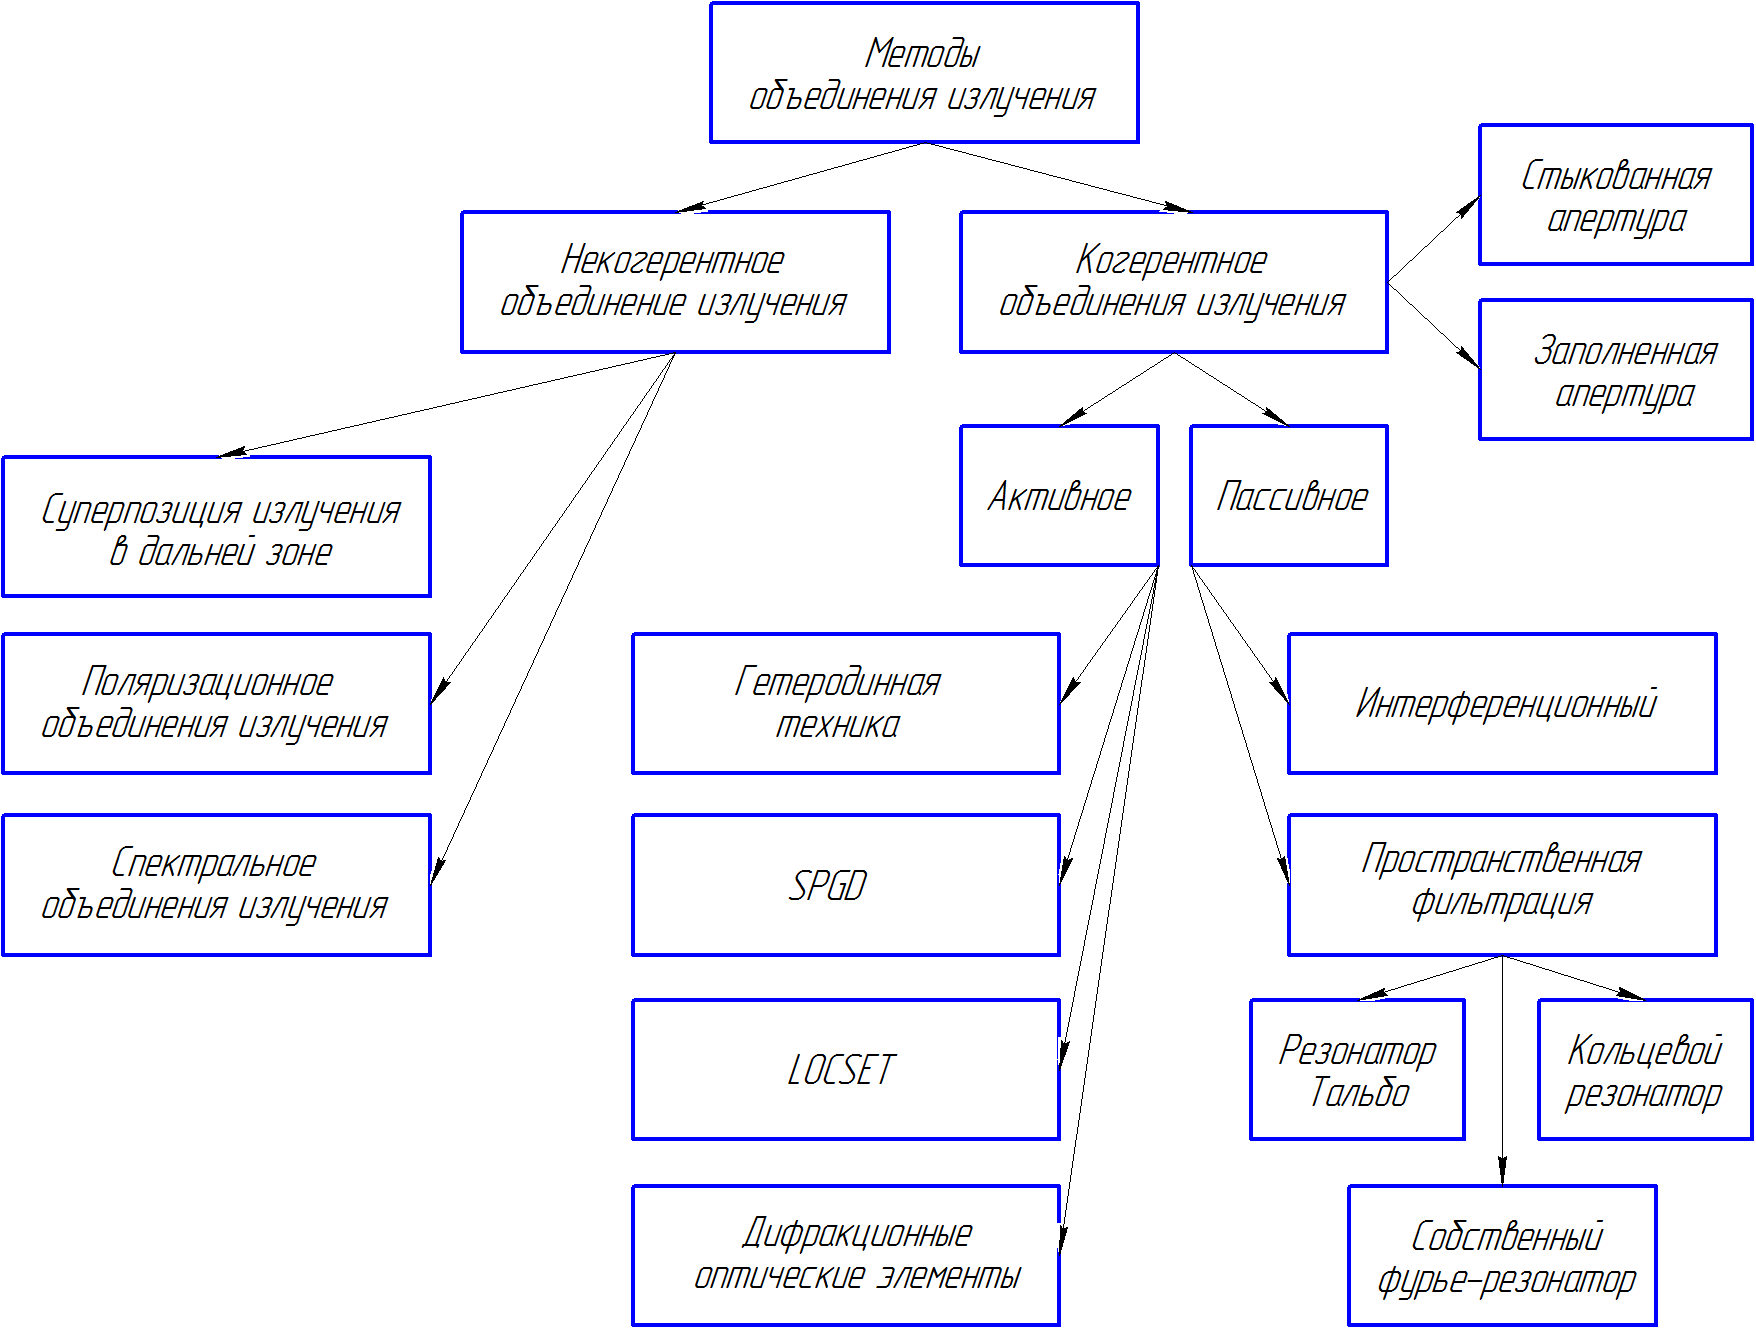
\includegraphics [scale=0.26] {jain_4_1}
  \caption{Классификация методов объединения излучения.}
  \label{img:jain_4_1}
\end{figure}

\section{Основные проблемы применения мощных волоконных лазеров}

Успешная разработка лазерного оружия обещает оказать глубокое влияние на будущие военные миссии. Лазерные системы направленного энергетического воздействия (НЭВ, DE в зарубежной терминологии) должна обеспечивать доставку сотен киловатт средней мощности до цели на километровые расстояния сквозь неблагоприятные атмосферные условия. Кроме того, лазерная система должна быть эффективной, компактной, устойчивой и надежной. Несмотря на значительный прогресс в данной области, цель на сегодняшний момент --- получить существенное увеличение мощности за счет развития технологий мощных волоконных лазеров. Мощные волоконные лазеры также могут быть применены в области доставки энергии, например, до спутников на низкой орбите и UAV, а также в оборонительных системах термосилового поражения наземного и космического базирования.

Для достижения максимальной (предельной) лазерной мощности необходимо объединить большое количество волоконных лазеров. Лазеры могут быть объединены когерентно, спектрально или некогерентно. Например, в настоящее время анализ открытых интернет-источников указывает на то, что военные исследования США сосредоточены на некогерентном объединении мощных волоконных лазеров с высоким оптическим качеством излучения. У этого подхода есть много преимуществ перед когерентным или спектральным объединением.

Ниже кратко приведены основные сведения из области распространения лазерного излучения в атмосфере, даны характеристики ряда мощных зарубежных волоконных лазеров и успехи, сделанные в направлении увеличения выходной мощности этих устройств, поддерживая при этом высокое оптическое качество. Кроме того, сравнивается эффективность распространения некогерентно объединенных массивов волоконных лазеров и когерентно объединенных массивов в реалистичных атмосферных условиях при распространении на километровые расстояния. Приведены результаты ряда зарубежных полевых экспериментов. В научно-исследовательской лаборатории ВМС США (NRL) четыре одномодовых оптоволоконных лазера с объединенной непрерывной мощность 6,2~кВт были некогерентно объединены на цели на расстоянии в 1,2~км. Суммарный объем, занятый этими четырьмя волоконными лазерами, включая источник питания, диодную накачку и волокна составляет менее 2~м$^3$. В этих экспериментах было передано в общей сложности 3~кВт излучения на расстоянии в 1,2~км до цели радиусом 10~см при половине предельной мощности лазеров. Эффективность распространения  в умеренно турбулентной среде составила $\approx 90$~\%~\cite{Jain96}.

\subsection{Распространение лазерных лучей в атмосфере}

Физические процессы, влияющие на распространение мощных лазерных лучей в атмосфере, сложны и взаимосвязаны. Эти процессы включают дифракцию, молекулярное/аэрозольное рассеивание и поглощение, турбулентность из-за колебаний плотности воздуха, тепловое цветение (см. пояснение ниже) и другие. Кратко рассмотрим эти физические процессы с целью оценки и сравнения эффективности распространения объединенных одномодовых и многомодовых оптоволоконных лазеров.

Минимальная площадь фокуса лазерного луча получается путем настройки фокусного расстояния. Оно равно расстоянию до цели $L$. Площадь фокуса лазерного луча на цели определяется как $R = \theta_{spread} L$, где угол $\theta_{spread}$ является суммой вкладов от дифракции $\theta_{diff}$, атмосферной турбулентности $\theta_{turb}$, механического дрожания $\theta_{jitter}$ и теплового цветения $\theta_{bloom}$. Тепловое цветение, то есть самодефокусировка лазера, вызванная поглощением и последующим нагревом воздуха, может быть частично смягчено, распространением в атмосферном окне передачи, где поглощение достаточно низкое. Длина волны волоконного лазера $\lambda = 1$,075~мкм находится вблизи узкого окна передачи водяного пара, центр которого находится вблизи $\lambda = 1$,045~мкм. В присутствии водных аэрозолей фактическое окно передачи расширяется и легко включает длину волны волоконного лазера. Для уровней лазерной мощности менее 100 кВт, и в зависимости от поперечного воздушного потока и атмосферного поглощения, тепловые эффекты цветения можно не учитывать~\cite{NRL3}. Тепловое цветение вблизи потока излучения может быть устранено с помощью поперечного воздушного потока~\cite{NRL5}. Ниже также будем пренебрегать малым механическим дрожанием и сконцентрируемся на доминирующих эффектах турбулентности и дифракции.

Сила атмосферной турбулентности описывается параметром $C_n^2$, который характеризует амплитуду колебаний плотности воздуха. Значение $C_n^2$ обычно находится в диапазоне от $10^{-15}$~м$^{-2/3}$ (слабая турбулентность) до $10^{-13}$~м$^{-2/3}$ (очень сильная турбулентность). Влияние турбулентности на распространении лазерного луча характеризуется параметром Фрида (поперечная длина когерентности) $r_0$, который является функцией $C_n^2$ и диапазона распространения. Параметр Фрида изменяется от десятков сантиметров для слабых условий турбулентности до долей сантиметра для сильной турбулентности. Угол распространения лазерного луча из-за атмосферной турбулентности равен $\theta_{turb} = 1$,6 $\lambda/\pi r_0$~\cite{NRL6, NRL7}.

\subsection{Сравнение распространения одномодового и многомодового лазерного излучения}

Дифракционный угол расхождения отдельного лазерного луча представляется как $\theta_{diff} = M^2 \lambda / (\pi r_0)$. Цель когерентного объединения состоит в том, чтобы снизить дифракционный угол распространения путем фазовой и поляризационной блокировки $N$ отдельных одномодовых  лазеров, таким образом увеличивая эффективную площадь пятна фокуса на величину $\sqrt{N}$. Для излучения одномодовых оптоволоконных лазеров, распространяющегося на большие расстояния, расхождение, вызванное турбулентностью доминирует над дифракционным расхождением, то есть, $\theta_{turb} \gg \theta_{diff}$, так как параметр Фрида обычно меньше, чем начальная площадь лазерного пятна $r_0 \ll R_0$. С другой стороны, для многомодовых волокон (M$^2 \gg$ 1), дифракционный угол расхождения может быть достаточно большим, то есть $\theta_{diff}>\theta_{turb}$. У данных различий между одномодовыми и многомодовыми волокнами есть важные следствия для их эффективности распространения и использования адаптивной оптики для снижения эффекта турбулентности. Для одномодовых волокон использование адаптивной оптики может существенно улучшить эффективность распространения. Однако, для многомодовых адаптивная оптика незначительно скажится на эффективности распространения, потому что основной вклад в угол расхождения --- от дифракции, вызванной плохим качеством излучения, то есть, высокого значения $M^2$.

Чтобы определить достоинства некогерентного объединения одномодовых и многомодовых лазеров для DE приложений, необходимо сравнить их эффективности распространения. Определим эффективность распространения как соотношение мощности на цели к полной переданной лазерной мощности. В остальном система волоконных лазеров имеет излучатель одинкового размера и однаковую суммарную мощность. В таблице~\ref{tbl_nrl_1} перечислены параметры четырех систем мощностью 100~кВт. Например, для случая 3~кВт на канал с $M^2$ = 1 для достижения суммарной мощности в 100~кВт необходимо 33 волоконных лазера ($N_{fiber}$). Соответствующие значения $M^2$ отражают тот факт, что для многомодовых лазеров при увеличении мощности волоконного канала его качество излучения уменьшается (увеличения $M^2$). В таблице~\ref{tbl_nrl_1} также дан радиус коллимирующих линз для отдельных волоконных лазеров ($R_0$). Во всех случаях радиус системы направленного излучения составляет 50 см, и цель  является круглым диском с площадью поверхности 100 см$^2$. На рис. 4 показана эффективность распространения для $M^2$ = 1, 7 и 38 в вакууме (рис.~\ref{img:nrl_fig4} (a)) и в турбулентной среде с $C_n^2 = 10^{-14}$~м$^{-2/3}$ (см. рис.~\ref{img:nrl_fig4} (b) и (c)). Во всех случаях излучение фокусируются на цель. Для распространения через турбулентную среду на рис. 4 приведена эффективность без адаптивной оптики (b) и с адаптивной оптикой (c). Адаптивная оптика была смоделирована путем увеличения параметра Фрида в четыре раза. Штрихованные кривые обозначают случай одиночного идеального гауссова излучения с начальной площадью пятна, равной радиусу системы направленного излучения, то есть, теоретический верхний предел для идеально когерентно объединенного излучения. Для расстояния менее 10~км в вакууме (рис.~\ref{img:nrl_fig4} (a)) и для условий с доминирующей турбулентностью  (рис.~\ref{img:nrl_fig4} (b)) у одномодового некогерентно объединенного примера излучения (красная кривая) эффективность распространения фактически идентична случаю когерентно объединенного излучения (пунктирная кривая), в то время как эффективность распространения различных многомодовых оптоволоконных лазеров значительно меньше. На рис.~\ref{img:nrl_fig4} также видно, что использование адаптивной оптики может значительно улучшить эффективность распространения объединенных одномодовых оптоволоконных лазеров, но имеет небольшой эффект при объединении многомодовых лазеров.
\begin{figure} [ht]
  \center
  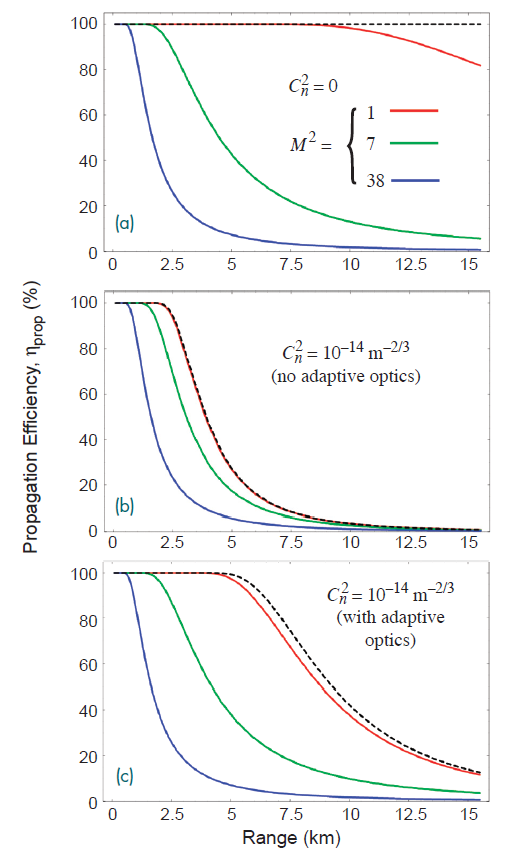
\includegraphics [scale=0.6] {nrl_fig4}
  \caption{График зависимости эффективности распространения от расстояния для некогерентно объединенных волоконных лазеров с  $M^2$ = 1, 7 and 38: (a) в вакууме, (b) в турбулентной атмосфере с $C_n = 10^{-14}$ м$^{-2/3}$ (без адаптивной оптики) и (c) в турбулентной атмосфере с адаптивной оптикой. Параметры лазеров приведены в таблице~\ref{tbl_nrl_1}. Пунктираня линия представляет теоретический верхний предел для когерентного и некогерентного объединения~\cite{Jain96}.}
  \label{img:nrl_fig4}
\end{figure}
\begin{table} [htbp]
  \centering
  \parbox{15cm}{\caption{Четыре конфигурации 100 кВт оптоволоконных одномодовых и многомодовых лазерных систем~\cite{Jain96}.}
  \label{tbl_nrl_1}}
  \begin{center}
  \begin{tabular}{| p{5cm} || p{2cm} | p{2cm} | p{2cm}l |}
  \hline
  \hline
  Мощность/волокно (кВт)   & \centering $M^2$ & \centering $N_{fiber}$ &\centering  $R_0$ (см) & \\
  \hline
  3 &\centering  1   &\centering  33    &\centering      8,7  &   \\
  5  &\centering  7   &\centering  20    &\centering      11,2  &   \\
  20 &\centering  38   &\centering  5    &\centering     22,4  &   \\
  100 &\centering  1   &\centering  1    &\centering     50  &   \\
  \hline
  \hline
  \end{tabular}
  \end{center}
\end{table}

\subsection{Критические характеристики базовых элементов мощных волоконных лазеров}
\label{sec_base_elem}

На сегодняшний день при создании мощных волоконных лазерных систем остро стоит вопрос об обладании технологиями производства даже базовых специализированных под высокую оптическую мощность элементов. В случае специфических методов объединения и использованной там элементной базы вопрос встает еще более остро. При любой поставленной конечной задаче (поразить цель, ослепить врага, разрезать металл и т.д.) ее решение будет заключаться не в конструкции волоконного лазера (схемы, параметры и геометрия волокна, методы накачки) и методах сложения излучения, а в доступной элементной базе. Насколько качественна и эффективна последняя, тем шире возможности по достижению высоких мощностей или выбору методов сложения излучения. На сегодняшний день чаще всего решается задача о том, как увеличить мощность лазера каким-либо способом исходя из имеющейся (в большинстве своем в продаже) элементной базы или имеющихся компетенций специалистов. Этот путь сам по себе возможен, но достаточно непродолжительный и быстро себя исчерпает.

Стратегически верным видится принципиальный акцент на создании качественного специального волокна, разработке и производстве большого спектра волоконно-оптических элементов, нанесении эффективных стойких оптических покрытий в рамках единой организационной структуры (в силу схожести и параллельности решаемых научно-технологических задач). Технологическая база для решения данной задачи в большинстве случаев имеется.

Ниже будут детально проанализированы основные методы построения мощных волоконных лазерных систем, а также выделены использованные волоконно-оптические, включая объемные, элементы (ВОЭ) и их необходимые характеристики. Важно отметить, что во всех описанных методах можно выделить общие для всех требования к использованным ВОЭ:
\begin{enumerate}
  \item Стойкость к воздействию (прохождению) мощного лазерного излучения с высокой яркостью.
  \item Использование стойких оптических покрытий.
  \item Отсутствие деградации оптических и механических (появление хрупкости, изменение размеров и формы) характеристик в течение всего срока службы системы (комплекса).
  \item Защита ВОЭ от воздействия внешних факторов.
  \item Оценка, учет и контроль термооптических (неравномерных по геометрии, неравномерных в многоэлементной системе) искажений ВОЭ при моделировании и конструировании.
  \item Однозначное наличие пассивной или активной системы охлаждения ВОЭ. При необходимости --- термостабилизация.
  \item Разработка и внедрение мер повышения надежности и отказоустойчивости ВОЭ и их систем в комплексах, требующих повышенного ресурса и работающих в сложных агрессивных условиях.
\end{enumerate}

В таблице~\ref{tbl_base_elem} приведены волоконные элементы, являющиеся общими и неотъемлемыми элементами современных мощных волоконных лазеров.
\begin{table} [htbp]
  \centering
  \parbox{15cm}{\caption{Базовые элементы мощных волокнных лазеров, общие для всех архитектур и методов объединения излучения.}
  \label{tbl_base_elem}}
  \begin{center}
  \begin{tabular}{| p{5cm} | p{5cm} | p{5cm} |}
  \hline
  \hline
  Наименование (тип)   & Использование & Характеристики \\
  \hline
  \hline
  Волоконные объединители накачки (<<каплеры>> при нестрогом использовании данного термина) & Объединение излучения модулей накачки и ввод его в активное волокно & Предельно малые оптические потери; максимальное количество каналов ввода излучения; минимальный размер выходного канала (диаметр оболочки)  \\
  \hline
  Волоконные брэгговские решетки или фотоиндуцированные решетки показателя преломления & Зеркала в резонаторе волоконного лазера   & Стоикость к высокой оптической нагрузке и нагреву \\
  \hline
  Активное оптоволокно & Активная среда в резонаторе волоконного лазера   & Высокий коэффициент поглощения на длине волны накачки; низкие потери на длине волны генерации; активное охлаждение из-за неизбежного нагрева, вызванного квантовым дефектом; минимальный квантовый дефект (вариации легирующих элементов); высокая эффективность генерации \\
  \hline
  Фильтры мод оболочки & Удаление излучения (оболочечные моды, непоглощенная накачка) из первой оболочки ВДО & Стоикость к  нагреву; эффективный теплосъем   \\
  \hline
  \hline
  \end{tabular}
  \end{center}
\end{table}


\section{Некогерентное объединение излучения}

Некогерентное объединение излучения использует  некогерентные в пространстве и по времени пучки излучения от нескольких излучателей (эмиттеров) с перекрытием их либо в дальней зоне, либо объединением их в одиночный дифракционно-ограниченный пучок излучения (все еще некогерентный по времени, но возможно пространственно когерентный) в ближней зоне. Это достигается путем использования методов суперпозиции пучков излучения в дальней зоне, поляризационного мультиплексирования, а также мультиплексирования длин волн лазерных массивов. \textit{Объединяя таким образом излучение N лазеров в лучшем случае можно увеличить интенсивность на оси в дальней зоне в N раз от интенсивности одиночного лазера}.

\subsection{Суперпозиция излучения в дальней зоне}

В этом методе выходные пучки излучения нескольких лазеров накладываются (взаимно перекрываются) в области цели без согласования относительных фаз, длин волн или поляризаций. Обычно, для формирования выходной апертуры выходные концы отдельных лазеров размещаются рядом. Далее, используя активную объемную оптику, отдельные пучки излучения направляются так, чтобы получить их взаимное перекрытие на цели в дальней зоне (см. рис.~\ref{img:jain_4_2})~\cite{Jain96}. Как сказано выше, при такой схеме, объединяя N лазеров можно в лучшем случае в дальней зоне получить излучение в N раз больше излучение одиночного лазерного пучка. При альтернативном подходе выходное излучение нескольких лазеров вводится в большее волокно, таким образом объединяя их в одной апертуре но с уменьшением качества пучка излучения.

\begin{figure} [ht]
  \center
  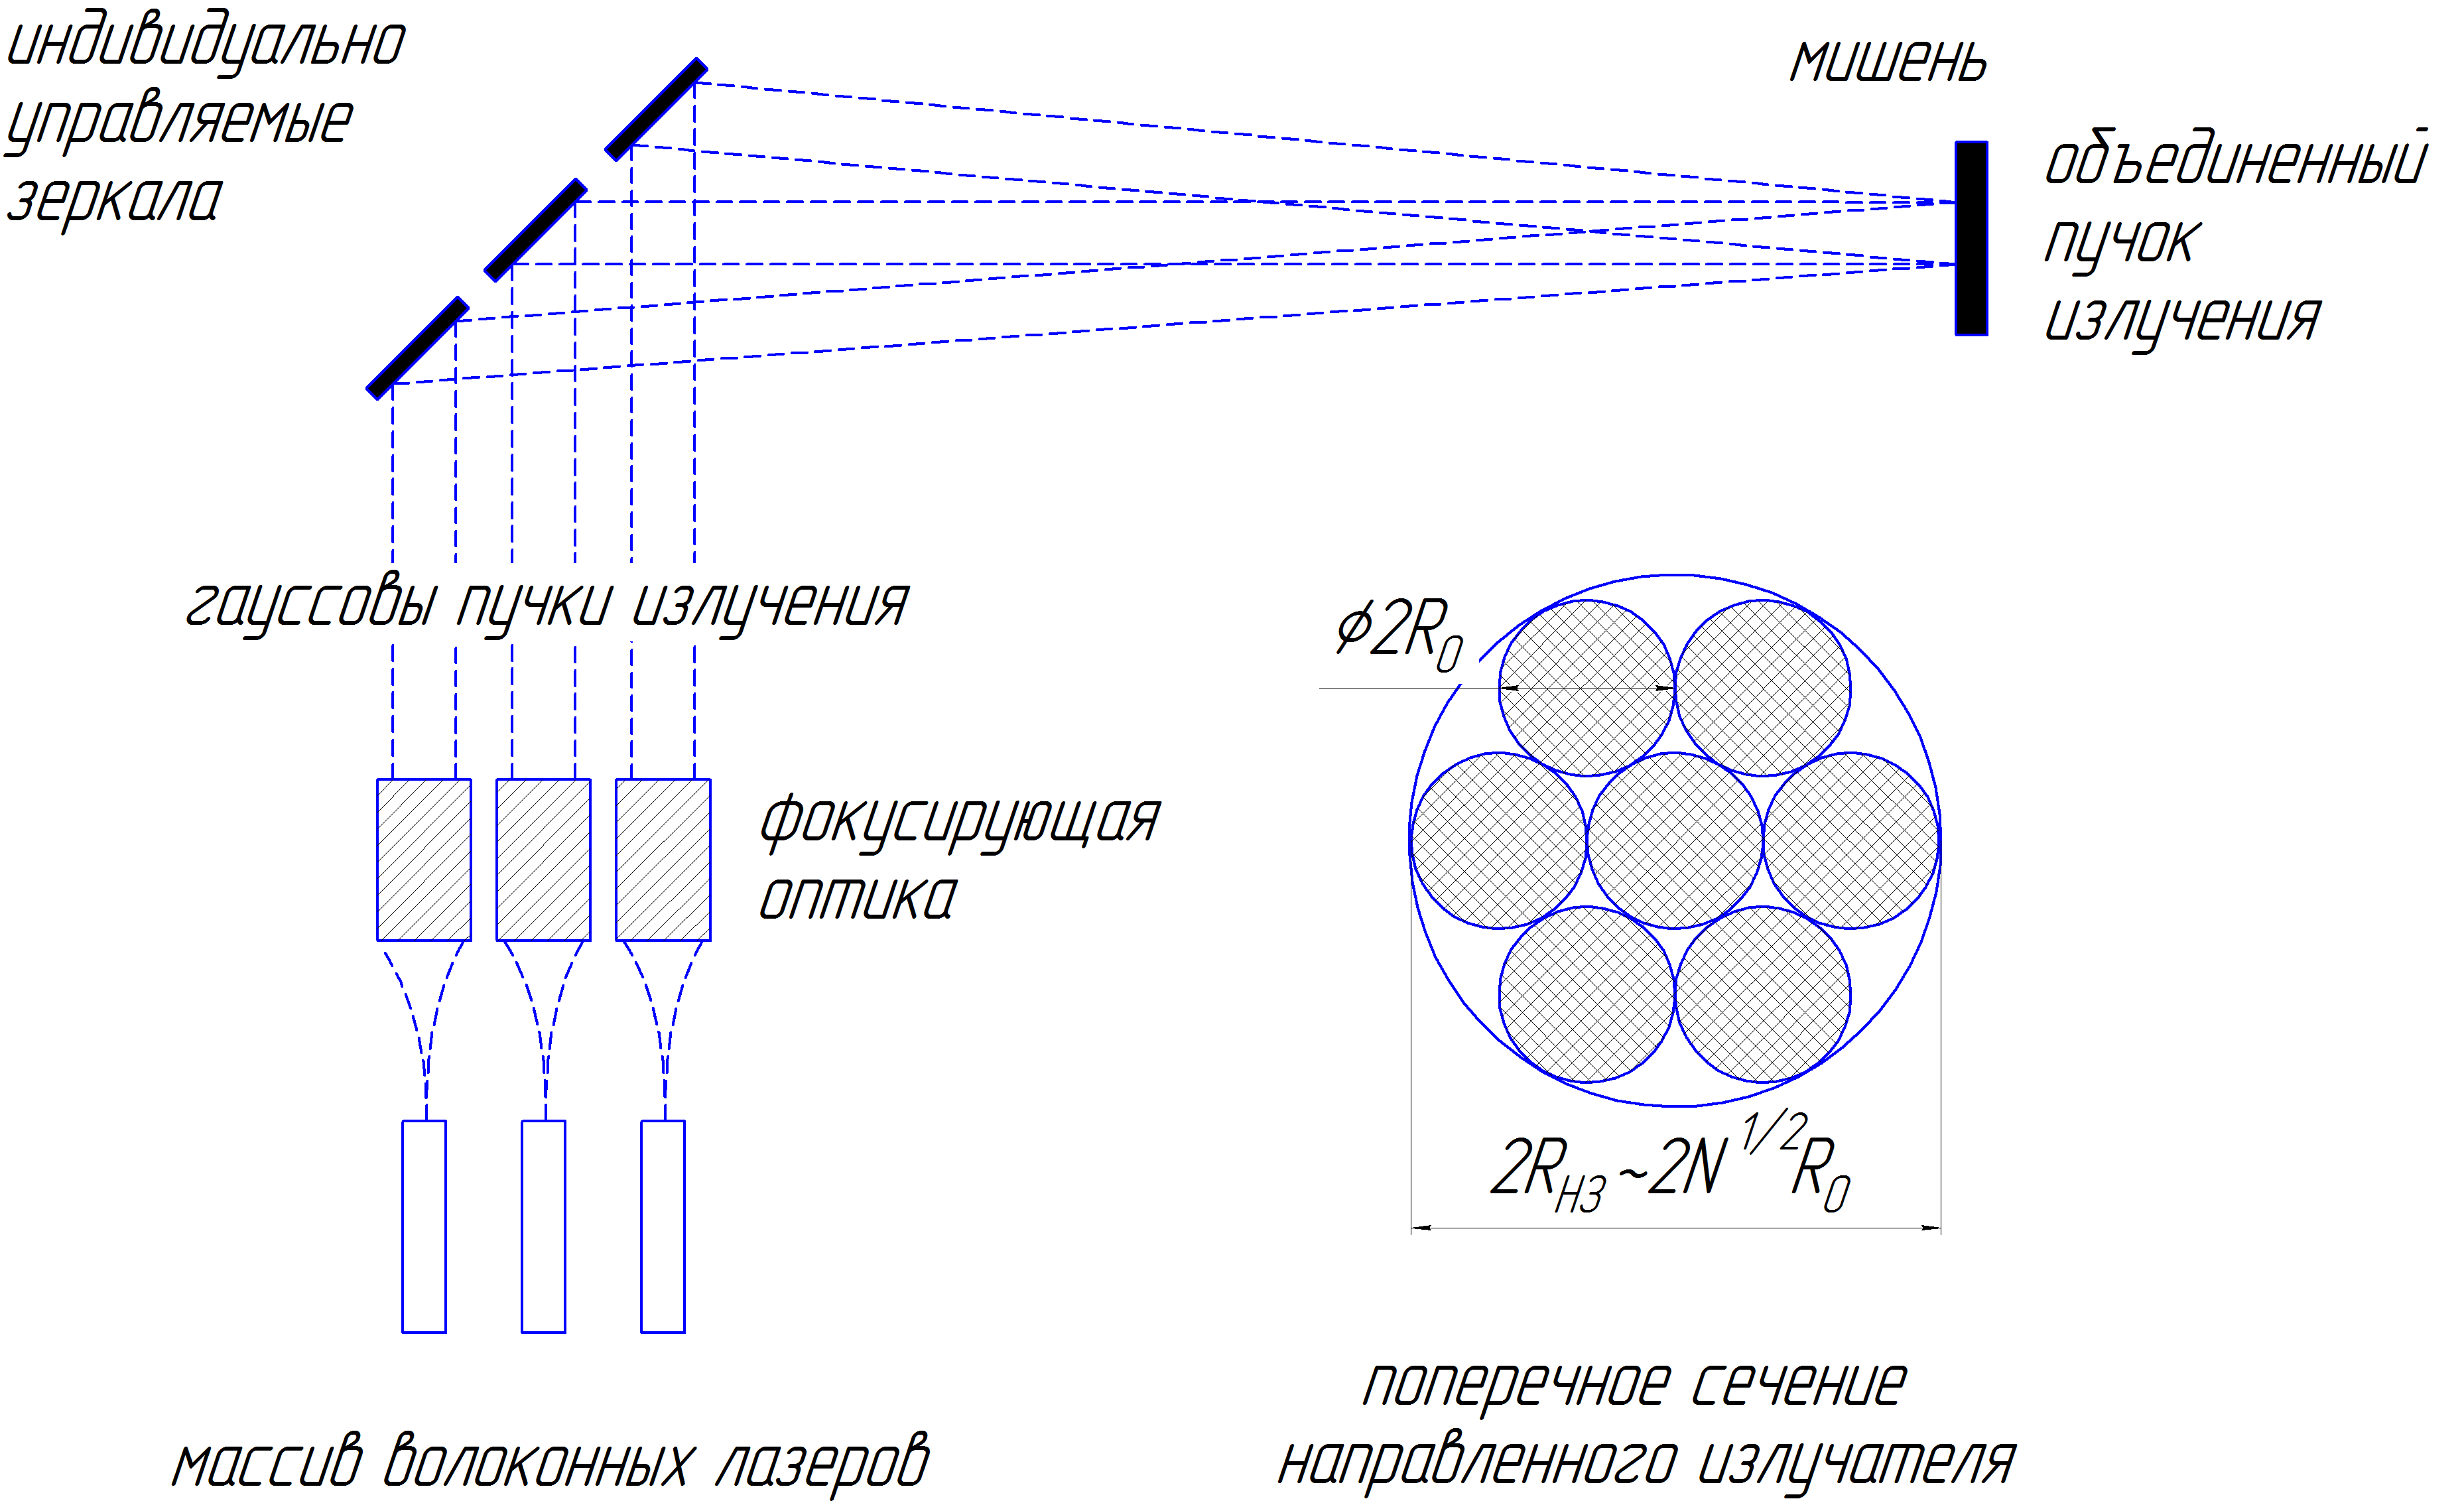
\includegraphics [scale=0.1] {jain_4_2}
  \caption{Некогерентное объединение излучения с помощью метода суперпозиции в дальней зоне.}
  \label{img:jain_4_2}
\end{figure}

Этот недорогой и простой метод использовался компанией IPG (США) для демонстрации их волоконного лазера мощностью 30-50~кВт с эффективностью <<от розетки>> 25-30~\%~\cite{Jain97}. В 2008 году в научно-исследовательской лаборатории ВМС США были некогерентно объединены четыре одномодовых оптоволоконных лазера IPG с общей выходной мощностью в 6,2~кВт на расстоянии 1,2~км~\cite{Jain96}.

В~\cite{Jain96} приведены результаты моделирования распространения лазерного излучения на большое расстояние с учетом атмосферной турбулентности для когерентного и некогерентного объединения излучения. Получено, что при типичных условиях для направленных энергетических применений соответствующие полезные действия почти идентичны. Эффективность распространения определялась как отношение мощности на цели к полной переданной мощности. Моделирование выполнялось для одного апертурного размера и размера цели в 100~см$^2$. На основе проведенного анализа авторы утверждают, что \textit{нет никаких существенных преимуществ для когерентного пучка излучения по сравнению с некогерентным объединением для приложений, требующих распространения излучения на большие расстояния в атмосфере}. Возможно самое важное преимущество этого метода --- отсутствие физических факторов, ограничивающих число объединяемых источников. Излучение на цели в значительной степени зависит от того, как точно могут управляться и фокусироваться отдельные пучки излучения, чтобы получить минимальное пятно перекрытия на цели. Это может потребовать использования многоэлементной и крупной активной оптики. В результате IBC (некогерентное объединение) обычно приводит к ухудшению качества результирующего пучка излучения и более низкой яркости объединенного излучения на цели по сравнению с отдельными исходными пучками излучения.

\begin{table} [htbp]
  \centering
  \parbox{16cm}{\caption{{Использованные волоконно-оптические элементы.}}
  \label{tbl_nrl_2}}
  \begin{center}
  \begin{tabular}{ | p{6cm} | p{9cm} |}
  \hline
  \hline
  Тип & Характеристики \\
  \hline
  \hline
    Активная объемная оптика & Большие габаритные размеры, прецизионное позиционирование, сложное электронное управление большими массивами элементов\\
  \hline
    Оптическое волокно & Большой диаметр (600-1500 мкм)  \\
  \hline
  \end{tabular}
\end{center}
\end{table}

\subsection{Поляризационное объединение излучения}

При поляризационном объединении излучения (ПОИ, PBC) два пучка излучения с ортогональной поляризацией объединяются с помощью чувствительной к поляризации оптики. В самом простом случае два линейно поляризованных лазера объединяются, используя поляризационный делитель пучка излучения (ПДП, PBS) в обратном направлении. ПОИ обычно используется, чтобы объединить два диодных лазера для осуществления накачки через свободное пространство твердотельных или волоконных лазеров, как показано на рис.~\ref{img:jain_4_3}. Этот метод \textit{сохраняет качество пучка излучения, увеличивая при этом его мощность}, таким образом способствуя масштабированию яркости. Однако, на практике крайне сложно с помощью ПОИ объединять больше двух источников и, следовательно, этот метод находит ограниченное применение в лазерах высокой мощности.

\begin{figure} [ht]
  \center
  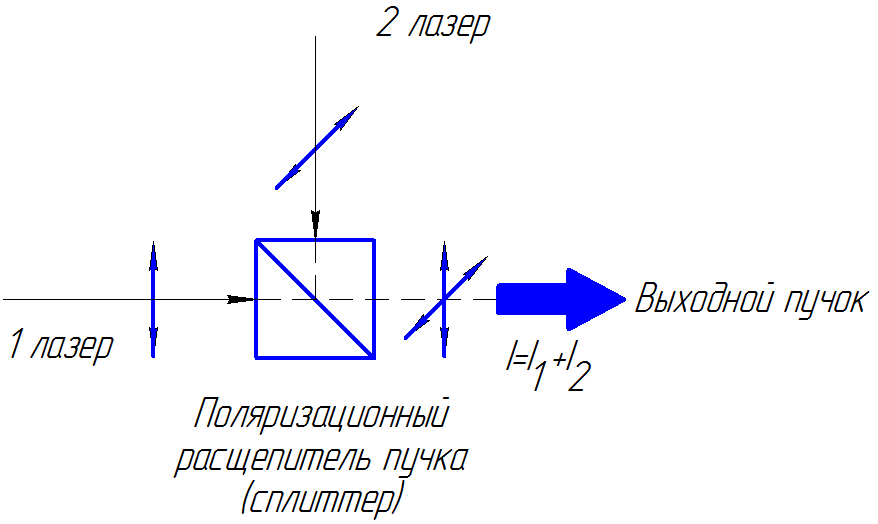
\includegraphics [scale=0.3] {jain_4_3}
  \caption{Схема поляризационного объединения излучения.}
  \label{img:jain_4_3}
\end{figure}

\begin{table} [htbp]
  \centering
  \parbox{16cm}{\caption{{Использованные волоконно-оптические элементы.}}
  \label{tbl_nrl_3}}
  \begin{center}
  \begin{tabular}{ | p{6cm} | p{9cm} |}
  \hline
  \hline
  Тип & Характеристики \\
  \hline
  \hline
    Объемная оптика (поляризационный делитель пучка) & Чувствительность к поляризации; точное механическое исполнение граней для качественного позиционирования \\
  \hline
    Поляризаторы & Адаптированность к работе с элементами в волоконном исполнении; собственное волоконное исполнение\\
  \hline
  \end{tabular}
\end{center}
\end{table}

Используя ПДП было продемонстрировано объединение излучения двух легированных иттербием волоконных лазеров с объединенной мощностью около 90~Вт~\cite{Jain98}. Несмотря на то, что для объединения использовались вращатели поляризации и ПДП, этот метод требует источников с различными длинами волн и ближе к спектральному объединению излучения. Поэтому данный метод как правило не выделяют в отдельный класс методов некогерентного объединения излучения.

\subsection{Спектральное объединение излучения}

При спектральном объединении излучения (СОИ) выходы массива источников, работающих на различных длинах волн, пространственно накладываются друг на друга посредством фильтров или дисперсионных элементов с формированием объединенного пучка излучения. Этот метод подобен разделению по длинам волн в мультиплексирующих системах, используемых в телекоммуникационных сетях. Принимая во внимание, что в системах связи используются волоконные элементы низкой мощности, в системах спектрального объединения излучения высокой мощности не обойтись без использования дифракционной оптики в свободном пространстве (так называемой объемной дифракционной оптики).

Системы спектрального объединения излучения могут быть разделены на \textit{последовательные} и \textit{параллельные} (см. рис.~\ref{img:jain_4_4}). Использование дихроических зеркал для перекрывания пучков излучения различных длин волн является примером последовательного СОИ, тогда как использование поверхностных решеток с многократными дифракционными порядками --- пример параллельного СОИ. Наиболее широкое распространение при спектральном объединении излучения получили дифракционные решетки в качестве мультиплексоров длин волн. Наряду с этим, было продемонстрировано несколько архитектур с использованием поверхностных и объемных решеток~\cite{Jain91,Jain99,Jain100,Jain101,Jain102,Jain103,Jain104,Jain105,Jain106,Jain107}. Эти подходы можно в общем классифицировать как системы с \textit{внешним} и \textit{общим резонаторами}.

\begin{figure} [ht]
  \center
  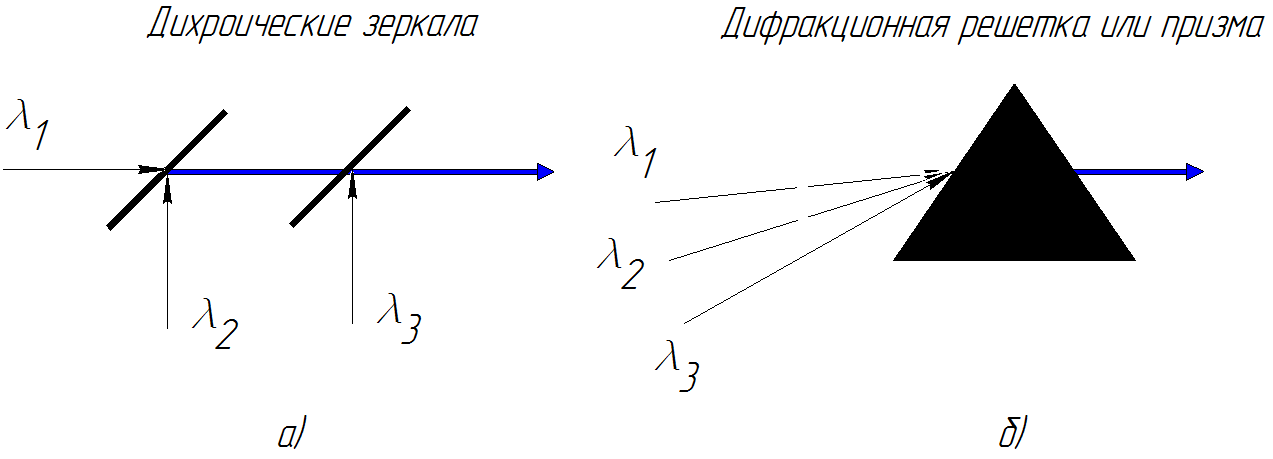
\includegraphics [scale=0.2] {jain_4_4}
  \caption{Спектральное объединение излучения: (а) последовательное, (б) параллельное.}
  \label{img:jain_4_4}
\end{figure}

В конфигурации с внешним резонатором каждый лазер в массиве работает на определенной длине волны с заданными интервалами по длинам волн между соседними лазерами. Эти задающие лазеры представляют собой одночастотные лазеры или волоконные лазеры в архитектуре ЗГ-У. Выход каждого лазера пространственно перекрывается с помощью дифракционных решеток, разработанных специально для данных длин волн и интервалов. Сообщалось о 2 кВт объединенной мощности с $M^2\approx 2$ после объединения 4 волоконных ЗГ-У лазеров с помощью диэлектрической решетки~\cite{Jain102}. Позднее отдельные усилители были масштабированы до мощности 2,1 кВт с объединенной мощностью в 8,2 кВт и $M^2$=4,3 ограниченным качеством пучка излучения отдельных усилителей~\cite{Jain108}. Эффективное СОИ (92 \%) пяти волоконных лазеров с объединенной выходной мощностью 770 Вт и качеством пучка излучения, ограниченным источниками, продемонстрировано, используя ОБР (VBG), записанные в ФТР (PTR) стекле~\cite{Jain91}. В этом эксперименте 4 ОБР использовались последовательно для объединения 5 пучков излучения как показано на рис.~\ref{img:jain_4_5}. Кроме того, была предложена архитектура с мультиплексированными ОБР, записанными на одной стеклянной подложке, чтобы сократить количество объединяющих элементов.

\begin{figure} [ht]
  \center
  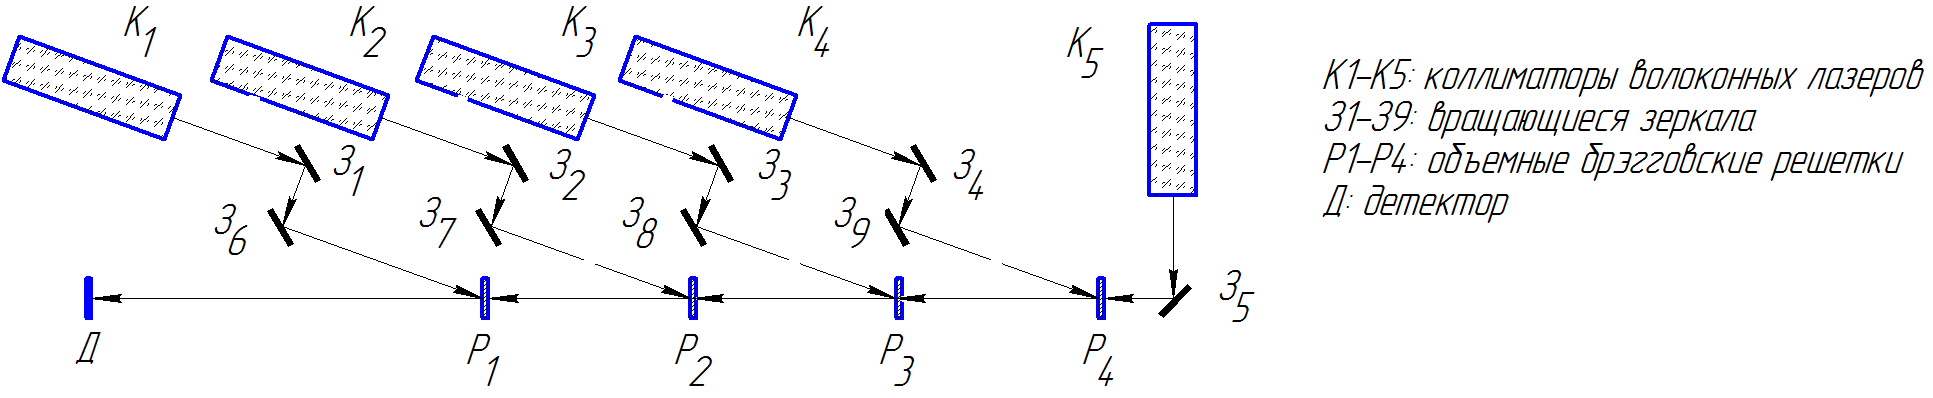
\includegraphics [scale=0.23] {jain_4_5}
  \caption{Пятиканальный СОИ с использованием объемных брэгговских решеток.}
  \label{img:jain_4_5}
\end{figure}

В подходе с общим резонатором (см. рис.~\ref{img:jain_4_6})~\cite{Jain103} у массива лазеров есть общий канал с обратной связью, сформированный решеткой и выходным связывающим зеркалом на одном конце. Излучение от каждого эмиттера в массиве падает на решетку под различным углом в зависимости от его позиции в массиве. Он определяет длину волны, которую решетка направляет к частичному отражателю, вынуждающему каждый эмиттер работать на уникальной позиционно-зависимой длине волны. В этом случае выходом является общий пучок излучения, состоящий из всех длин волн. Объединение достигается без внешнего контроля за длинами волн и шириной спектральной линии каждого эмиттера.

\begin{figure} [ht]
  \center
  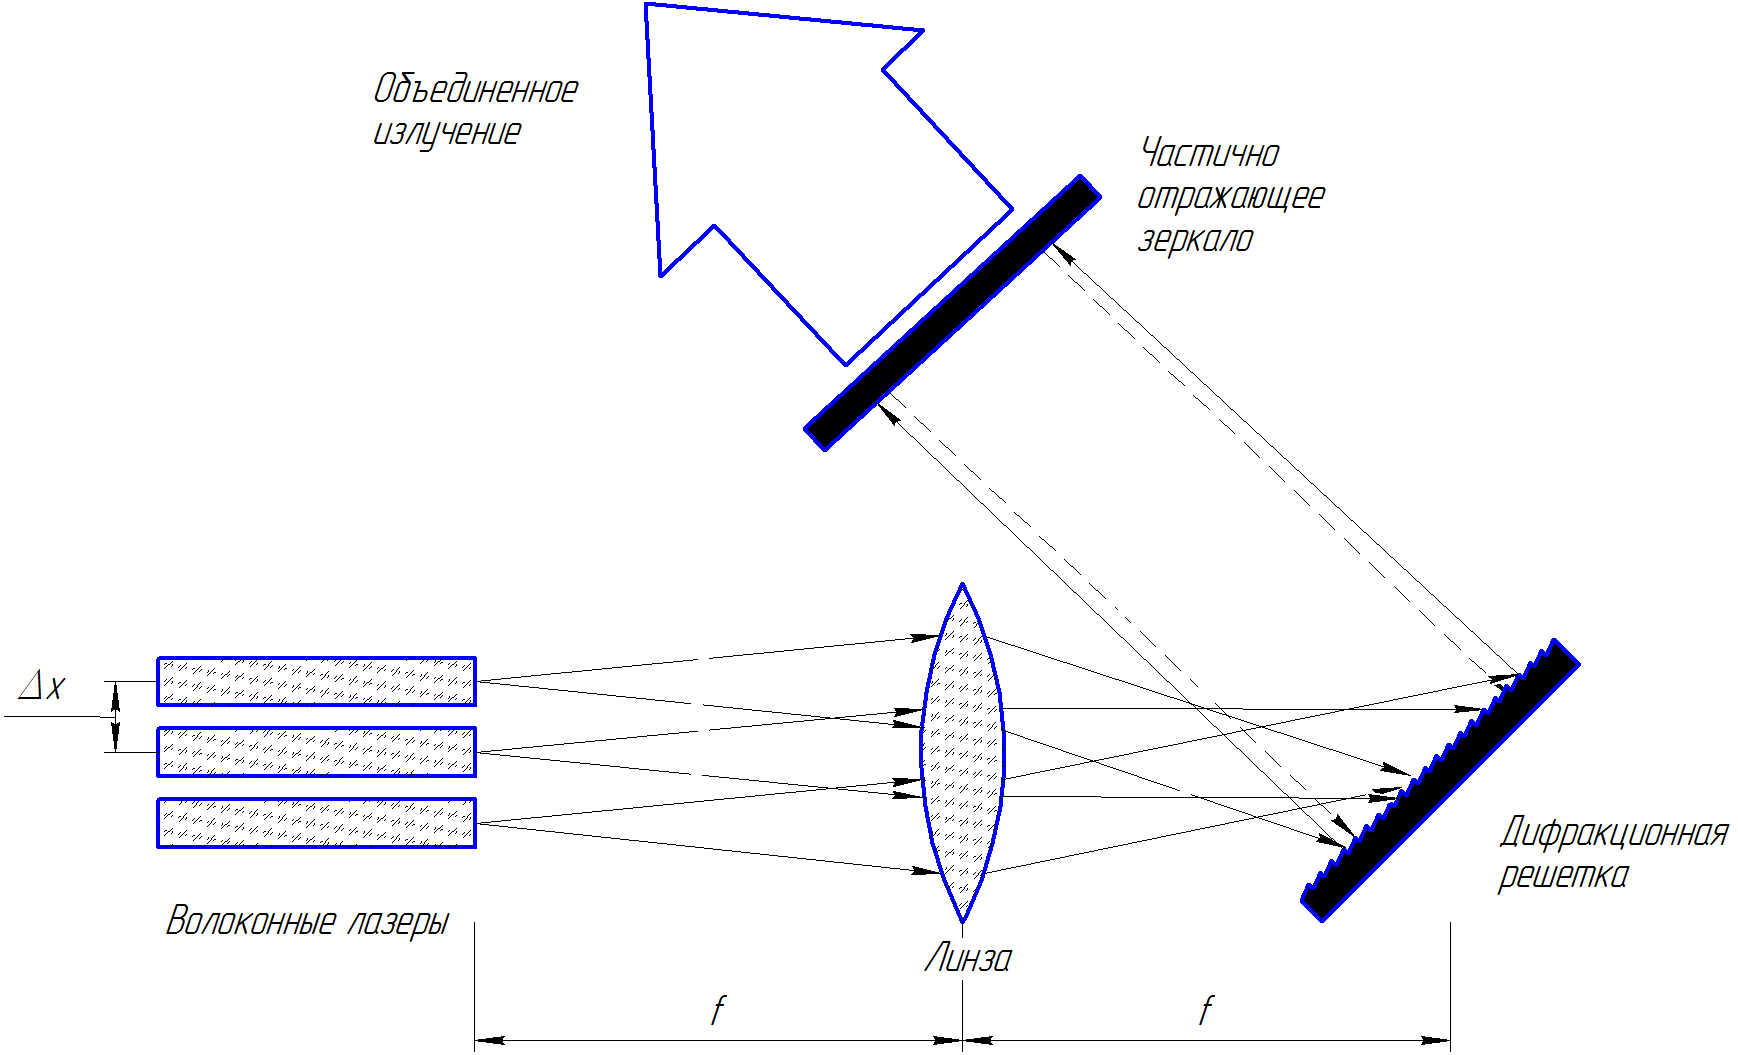
\includegraphics [scale=0.23] {jain_4_6}
  \caption{Схема СОИ с общим резонатором.}
  \label{img:jain_4_6}
\end{figure}

При другом подходе для того, чтобы объединить пучки излучения с различными длинами волн, используются поляризаторы, зависящие от длины волны~\cite{Jain98}. Этот метод был продемонстрирован при объединении двух волоконных лазеров, которые были спектрально разделены на 28 нм. Возможность масштабирования большего массива пока не ясна. Сообщалось о некоторых предварительных попытках использовать несколько пространственно некогерентных пучков излучения, работающих на различных частотах, чтобы сгенерировать дифракционно-ограниченный одиночный пучок излучения, используя ВРМБ (SBS) в оптических волокнах~\cite{Jain109}. Два пучка излучения накачки, введенные в одномодовое волокно, возбуждали собственные отдельные стоксовы пучки излучения и производили одиночный пространственно когерентный пучок. Пока они лежат в окне пропускания материала волокна этот метод позволяет комбинировать лазеры без любого ограничения по длинам волн.

\textit{Методы СОИ позволяют масштабировать мощность с сохранением качества пучка излучения, но за счет спектральной яркости}. Есть несколько факторов, ограничивающих мощность и масштабируемость канала методов СОИ. Методы СОИ требуют источников с узкой шириной спектральной линии, с очень устойчивыми длинами волн и контролируемым интервалом. Узкая ширина спектральной линии приводит к снижению порогов нелинейности в волокнах, в то время как интервал по длинам волн определяет необходимые пределы числа лазеров в массиве из-за ограничения спектральной ширины усиления активной среды. В большинстве методов СОИ число оптических элементов в системе увеличивается с увеличением числа лазеров в массиве. Это приводит к дополнительным потерям в системе, повышению сложности выравнивания и увеличению размера системы в целом. Большое количество оптических элементов также приводит к серьезной тепловой нагрузке и необходимости ее решения, причем различные оптические элементы в системе по-разному разогреваются, что в свою очередь порождает нежелательные искажения при объединении пучков излучения.

\begin{table} [htbp]
  \centering
  \parbox{16cm}{\caption{{Использованные волоконно-оптические элементы.}}
  \label{tbl_nrl_4}}
  \begin{center}
  \begin{tabular}{ | p{6cm} | p{9cm} |}
  \hline
  \hline
  Тип & Характеристики \\
  \hline
  \hline
    Объемная оптика & Точное механическое исполнение; возможность точного позиционирования и настройки положения (требование к оправке) \\
  \hline
    Дифракционная объемная оптика: поверхностные или объемные решетки, призмы & Точная настройка на работу на заданной длине волны; устойчивая спектральная ширина \\
  \hline
    Зеркала: стандартные объемные или дихроические & \textit{без особых требований, кроме указанных в пункте~\ref{sec_base_elem}}\\
  \hline
    Поляризаторы & Адаптированность к работе с элементами в волоконном исполнении; собственное волоконное исполнение\\
  \hline
  \end{tabular}
\end{center}
\end{table}

\section{Когерентное объединение излучения}

% section section_name (end)

При когерентном объединении излучения (КОИ, CBC) несколько лазерных источников некоторым образом фазируются друг относительно друга, что вынуждает их испускать взаимно когерентное излучение. Для достижения этого подбираются илиподстраиваются относительные фазы, длины волн и поляризации отдельных объединяемых источников. В приложениях, требующих высоких мощностей, предложено большое количество методов когерентного объединения излучения лазеров.

\subsection{Стыкованная и заполненная апертуры}

Методы когерентного объединения излучения могут быть разделены на \textit{активные} или \textit{пассивные} в зависимости от того, как осуществляется блокировка фазы в массиве источников. При активном КОИ с помощью оптоэлектронных средств обратной связи в режиме реального времени контролируется фаза каждого из источников. Естественно это требует сложной электроники и фазо-измерительного оборудования. С другой стороны, при пассивном КОИ источники обычно имеют общий резонатор и самоорганизуются для испускания когерентного пучка без какой-либо внешней регулировки фазы. Это делает систему намного более простой и компактной.

В зависимости от конструкции резонатора методы КОИ также разделяются на методы со \textit{стыкованной} и \textit{заполненной апертурой}. При стыкованной апертуре отдельные лазерные подапертуры складываются в 2D массив с  формированием большой объединенной апертуры. В дальней зоне качество пучка излучения ограничивается коэффициентом заполнения 2D массива и часто приводит к нежелательным боковым <<хвостам>>, что снижает мощность в центральной части апертуры. С другой стороны, в конструкциях с заполненной апертурой выходы лазерных источников объединяются в общий резонатор и объединенный выход извлекаются из одиночной выходной апертуры. При такой конструкции может быть достигнуто качество дифракционно-ограниченного пучка излучения. Кроме различий в качестве пучка излучения конструкция не предлагает очевидных преимуществ с точки зрения числа фазируемых элементов. Обе конструкции активно использовались при демонстрации активных и пассивных систем КОИ.

Чтобы оценить потерю мощности в боковых <<хвостах>>, будем считать, что массив волоконных лазеров со стыкованной апертурой имеет шестиугольную геометрию (как показано на рис.~\ref{img:jain_4_7} для семи источников).

\begin{figure} [ht]
  \center
  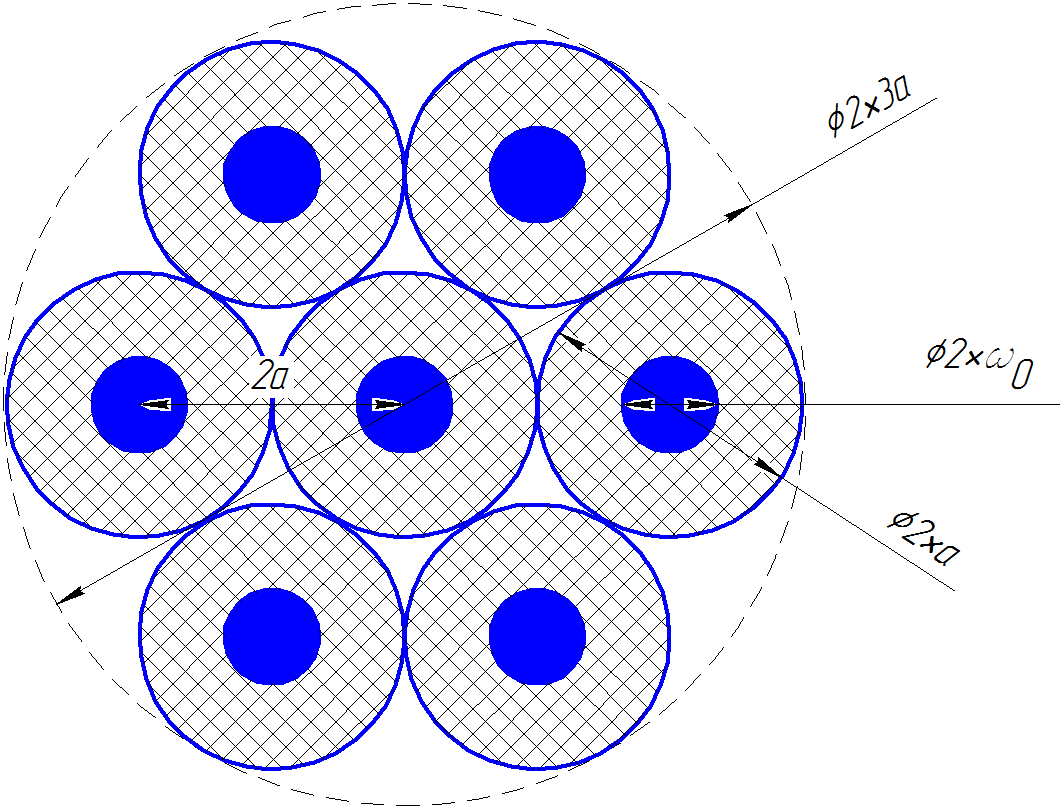
\includegraphics [scale=0.2] {jain_4_7}
  \caption{Шестиугольная стыкованная апертура с 7 подапертурами радиуса $a$. Каждая подапертура испускает гауссов пучок излучения с радиусом $\omega_0$.}
  \label{img:jain_4_7}
\end{figure}
Предположим, что выход каждой подапертуры с радиусом $a$ есть гауссов пучок излучения с нормализованной амплитудой $A(x,y)=\exp(-(x^2+y^2)/\omega_0^2)$, где $\omega_0 \ll a$ --- радиус пучка излучения. В реальной ситуации $\omega_0$ может быть радиусом поля моды самого низкого порядка в сердцевине одиночного волокна и $a$ --- радиус внешней оболочки используемого волокна. Эффективный коэффициент заполнения такого массива может быть определен как соотношение общей площади пучков излучения к площади полной апертуры. Например, в массиве из 7 элементов это
\begin{equation}\label{eq4.2-1}
  F=\frac{7\times\pi\omega_0^2}{\pi(3a)^2}.
\end{equation}
\noindent
В дальней зоне распределение интенсивности одиночной подапертуры с гауссовым распределением амплитуды (при игнорировании конечных апертурных эффектов для $\omega_0 \ll a$) дается преобразованием Фурье (ПФ)
$$
I_{F}(x,y;z)=\left[\left.\frac{1}{\lambda z}\mathcal F\{A(x,y)\}\right|_{u=\frac{2\pi x}{\lambda z}, \nu=\frac{2\pi y}{\lambda z}}\right]^2.
$$
Известно, что ПФ гауссианы является гауссианой, поэтому можно записать
\begin{equation*}
\begin{split}
\mathcal F\{A(x,y)\}&=\iint\exp\left(-\frac{x^2+y^2}{\omega_0^2}\right)\times\exp(-i(ux+\nu y))dx dy= \\
&=\pi\omega_0^2\times\exp\left[-\frac{\omega_0^2}{4}(u^2+\nu^2)\right],
\end{split}
\end{equation*}
\begin{equation}\label{eq4.2-2}
  I_{F}(x,y;z)=\left[\frac{\pi\omega_0^2}{\lambda z}\times\exp\left\{-\frac{\pi^2\omega_0^2}{\lambda^2z^2}(x^2+y^2)\right\}\right]^2.
\end{equation}
Теперь шестиугольная апертура с 7 элементами может быть представлена как свертка одиночной апертуры со смещенной дельта-функцией Кронекера
\begin{equation}\label{eq4.2-3}
  A_{arr}(x,y)=\exp\left(-\frac{x^2+y^2}{\omega_0^2}\right)\times f(x,y),
\end{equation}
где
\begin{equation*}
\begin{split}
  f(x,y)&=\delta(x,y)+\delta(x-2a,y)+\delta(x+2a,y)+\\
            &+\delta(x-a,y-\sqrt{3}a)+\delta(x+a,y-\sqrt{3}a)+\\
            &+\delta(x-a,y+\sqrt{3}a)+\delta(x+a,y+\sqrt{3}a).
\end{split}
\end{equation*}
Допуская, что выходы каждой подапертуры являются \textit{взаимно когерентными и синфазными}, распределение интенсивности в дальней зоне будет интерференционной картиной, сформированной всеми составляющими. В дальней зоне интерференционная картина --- простое фурье-преобразование апертуры. Отметим, что ПФ свертки двух функций --- произведение ПФ отдельных функций. Используя это свойство и ПФ смещенной дельта-функции $\mathcal F\{\delta(x-x_0,y-y_0)\}=\exp(-i(x_0u+y_0\nu))$ с некоторыми упрощениями ПФ $f(x, y)$ будет иметь вид
$$
\mathcal F\{f(x,y)\}=1+2\cos(2au)+4\cos(au)\cos(\sqrt{3}a\nu).
% здесь было ...\сqrt{3}..., я исправил на \sqrt{3} НАДО ПРОВЕРИТЬ КАК В ОРИГИНАЛЕ
$$
Затем, интенсивность массива в дальней зоне
\begin{equation}\label{eq4.2-4}
\begin{split}
  &I_{F_{arr}}(x,y;z)=\left[\left.\frac{1}{\lambda z}\mathcal F\{A(x,y)\}\times\mathcal F\{f(x,y)\}\right|_{u=\frac{2\pi x}{\lambda z}, \nu=\frac{2\pi y}{\lambda z}}\right]^2= \\
  &=\left[\frac{\pi \omega_0^2}{\lambda z}\exp\left\{-\frac{\pi^2\omega_0^2}{\lambda^2z^2}(x^2+y^2)\right\}\times\left\{1+2\cos\left(\frac{4\pi ax}{\lambda z}\right)+4\cos\left(\frac{2\pi ax}{\lambda z}\right)\cos\left(\frac{2\sqrt{3}\pi ay}{\lambda z}\right)\right\}\right]^2
\end{split}
\end{equation}
Подставляя в это уравнение $x=y=0$, т.е. имея в виду интенсивность на оси в дальней зоне, видим, что она всегда масштабируется как $7^2$, то есть $N^2$ в общем случае , независимо от коэффициента заполнения для когерентной стыкованной апертуры.

Обычно упоминаемое преимущество КОИ по сравнению с IBC состоит в том, что для апертур того же самого размера, излучение на оси в дальней зоне масштабируется как фактор $N$ для IBC и как фактор $N^2$ для КОИ, где $N$ --- число лазерных источников в объединяемом массиве. Это истина, когда размер каждой подапертуры при увеличении их числа сохраняется постоянным (размер полной увеличеной апертуры пропорционален $N$)~\cite{Jain46}. Это можно продемонстрировать используя модель, разработанную для массива стыкованных апертур с 7 элементами. Если теперь будем рассматривать его как массив взаимно некогерентных лазеров, направленных на цель в дальней зоне, выходы различных подапертур не смешиваются (интерферируют) друг в друга и просто накладываются в дальней зоне. В дальней зоне интенсивность определяется как $N$ интенсивностей одиночной апертуры (уравнение \eqref{eq4.2-2}).

На рис.~\ref{img:jain_4_8} дано сравнение распределение интенсивности в дальней зоне когерентного массива стыкованных апертур, некогерентного массива стыкованных апертур и когерентного массива заполненной апертуры с равными эффективными площадями мод и значениями $2a=125$~мкм и $2\omega_0=20$~мкм. Отметим, что пиковая интенсивность для обоих когерентных случаев одна и то же. Однако, в случае массива со стыкованными апертурами значительная мощность теряется в боковых  <<хвостах>> по сравнению с заполненной апертурой. Суммарная мощность в центральной части пучка в дальней зоне при гауссовом распределении и заполненной апертуре составляет 86,5 \% по сравнению с теоретическим пределом в 70 \% для максимальной мощности в центральной части от максимально возможной для архитектуры со стыкованной апертурой того же размера~\cite{Jain46}. Кроме того, нужно отметить, что общая мощность равна во всех случаях. Однако, в когерентном случае больше мощности концентрируется в малой центральной части пучка (явление самофокусировки) по сравнению с некогерентным случаем.

\begin{figure} [ht]
  \center
  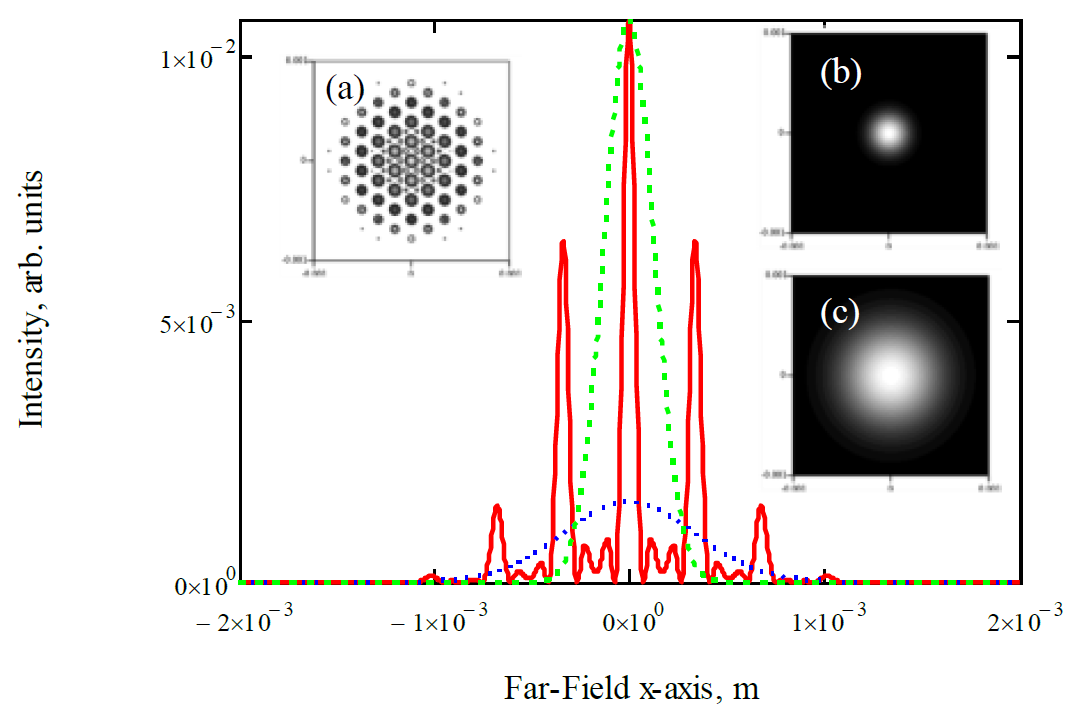
\includegraphics [scale=0.4] {jain_4_8}
  \caption{Распределение интенсивности в дальней зоне для (a) когерентной стыкованной апертуры (красная сплошная кривая); (b) когерентная заполненная апертура с равной площадью моды (зеленая штрихованная кривая), (c) некогерентная стыкованная апертура (синяя пунктирная кривая). Здесь в случае стыкованных апертур $2a=125$~мкм и $2\omega_0=20$~мкм~\cite{Jain46}.}
  \label{img:jain_4_8}
\end{figure}

\subsection{Активное когерентное объединение излучения}

Активный КОИ использует оптоэлектронную обратную связь в реальном времени для обеспечения испускания массивом усилителей  взаимно когерентного и синфазного излучение. На рис.~\ref{img:jain_4_9} показана общая схема активной системы КОИ, основанной на архитектуре ЗГ-У. У этой системы есть две ключевых части --- основной задающий генератор и массив оптических усилителей с  электроникой для активного фазирования. Задающий генератор обычно включает в себя одночастотный малошумящий полупроводниковый лазер и несколько этапов предварительного усиления, разделенных изоляторами. Его выход разделяется на равные части и усиливается в отдельных оптических усилителях. Стоит обратить особое внимание на то, чтобы длины всех усилителей в массиве были равны. Это критически важно по двум причинам: во-первых --- различие в длине должно быть меньше, чем длина когерентности задающего лазера (чтобы выходы усилителей были взаимно когерентными); во-вторых --- согласовать усиление в каждом усилительном каскаде так, чтобы уровни выходной мощности были максимально равными. Точная настройка длины оптического пути достигается через механизм регулировки в режиме реального времени, используя электронную обратную связь. Синфазные и взаимно когерентные выходы массива усилителей со стыкованными апертурами используя массив микролинз коллимируются и объединяются в дальней зоне.

\begin{figure} [ht]
  \center
  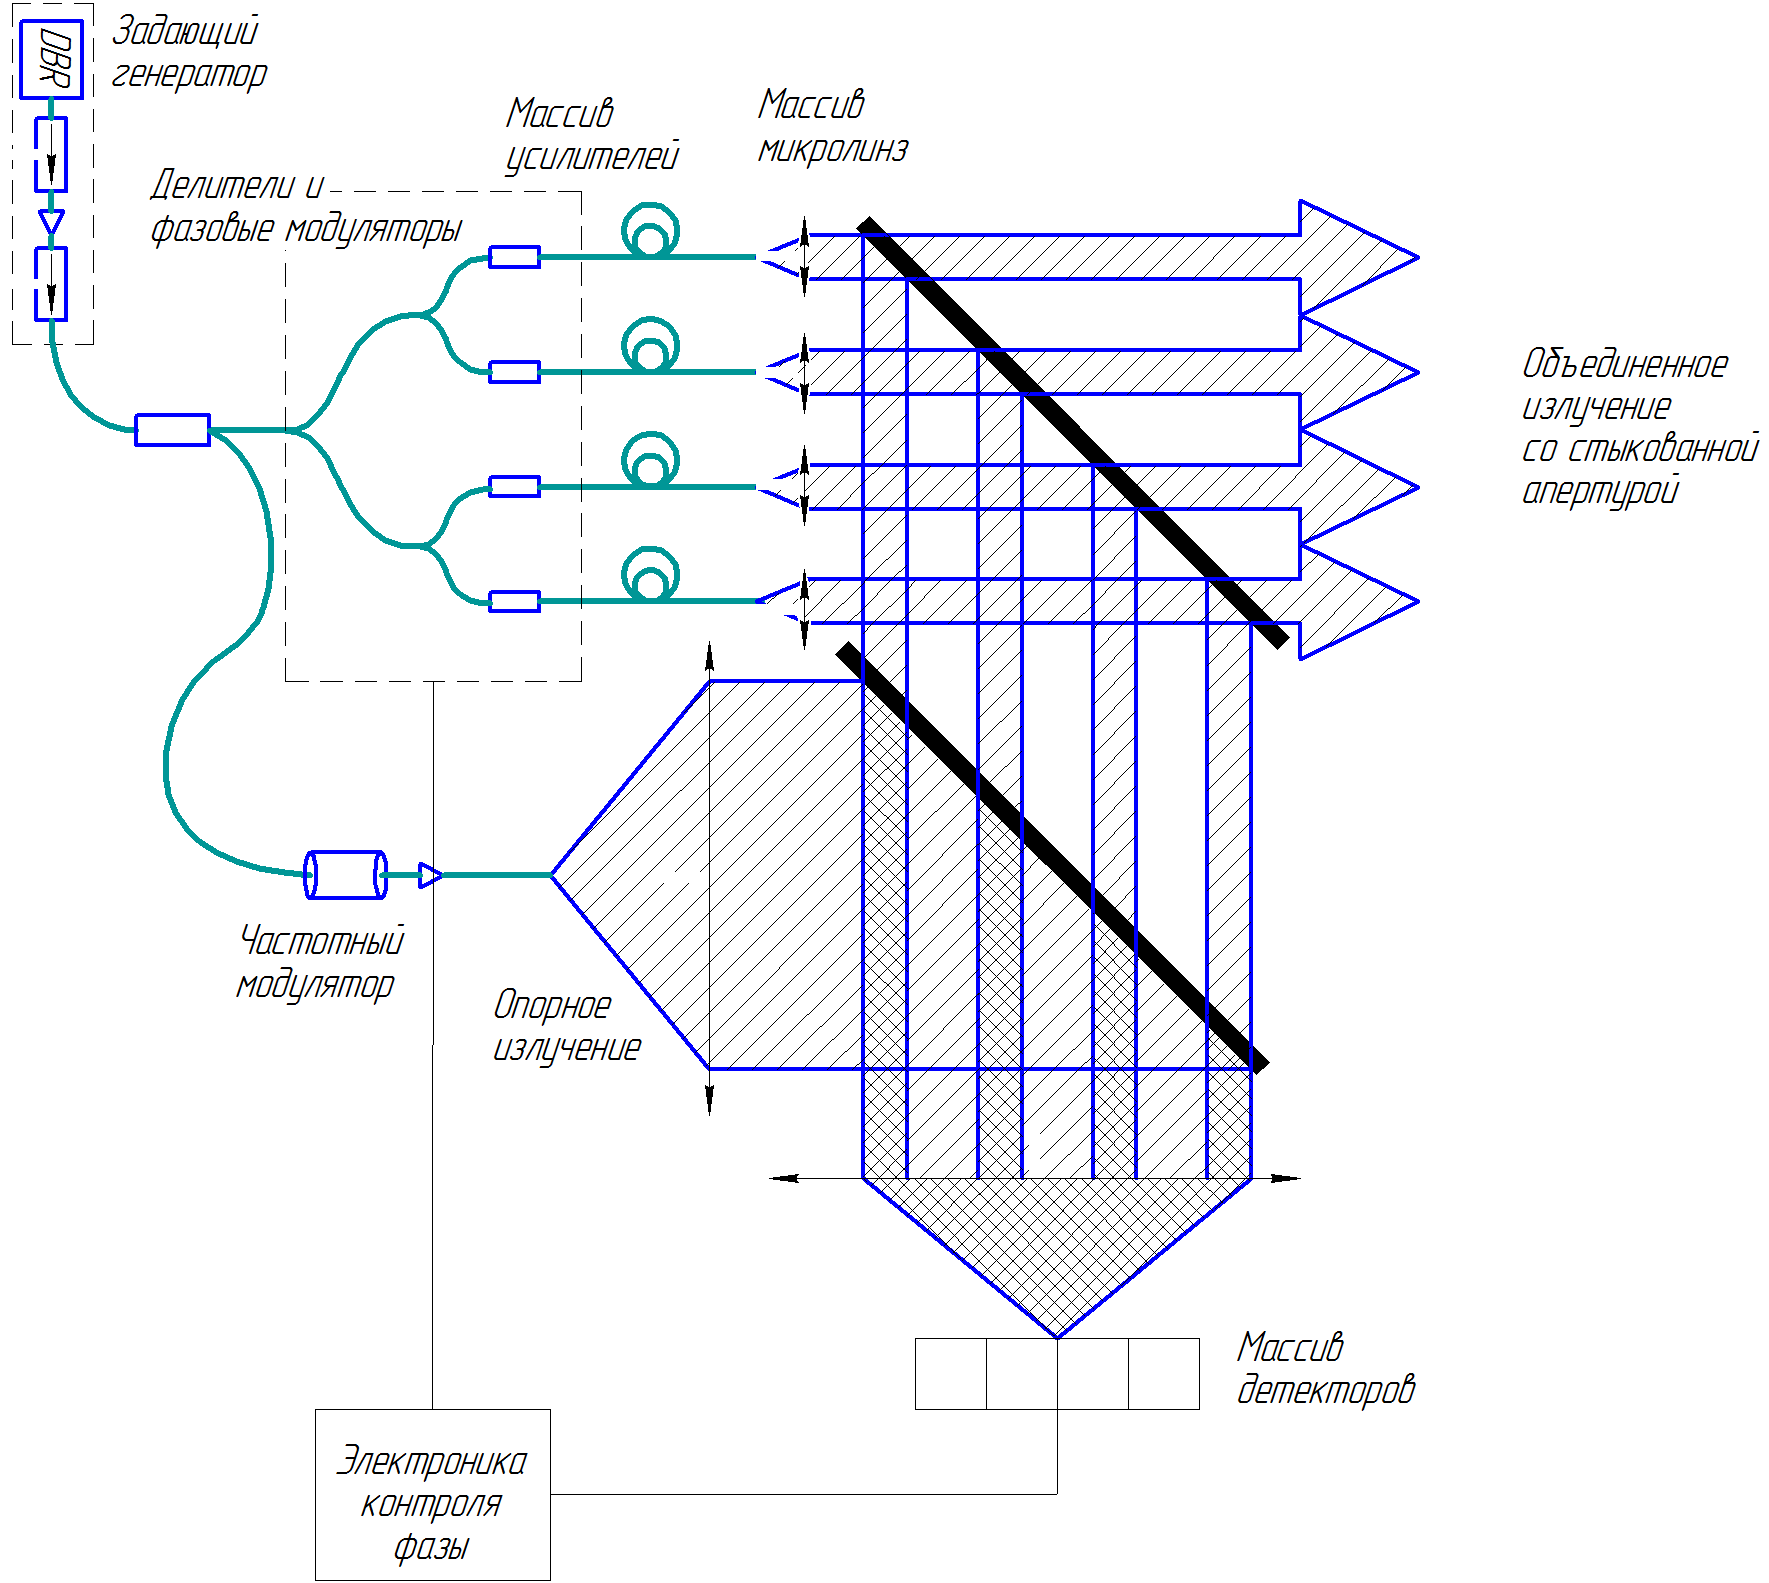
\includegraphics [scale=0.26] {jain_4_9}
  \caption{Общая схема реализации активной системы КОИ основанной на ЗГ-У.}
  \label{img:jain_4_9}
\end{figure}

Ранее было предложено несколько методов реализации активного механизма контроля, регулировки и обратной связи. Обычно, часть задающего сигнала смещается по частоте и смешивается с выходами массива оптических усилителей в разделителе пучка излучения (гетеродинная техника). Это приводит к появлению гетеродинных сигналов с биениями на частоте сдвига. С помощью массива фотодетекторов от каждого пучка излучения получается фазовая информация о биениях, которая используется, чтобы сгенерировать электронные сигналы об ошибке для фазовых контроллеров. В некоторых системах генерируются многократные активные сигналы обратной связи, чтобы управлять различными аспектами системы, такими как относительные фазы, поляризация и уровень выходной мощности. Широко используются два метода обнаружения и обработки сигналов: блокировка оптической когерентности одиночным детектором с тэгированием электронной частоты (locking of optical coherence by single-detector electronic frequency tagging, LOCSET)~\cite{Jain110} и стохастический параллельный метод градиентного спуска (stochastic parallel gradient descent, SPGD)~\cite{Jain111, Jain112}. Ниже рассмотрим их более подробно. В работах~\cite{Jain113, Jain114} также разработаны ряд методов активной блокировки фазу, не требующих задающего сигнала.

Известно об использовании активного метода КОИ на основе ЗГ-У со стыкованными апертурами для фазовой блокировки больших массивов~\cite{Jain113, Jain115} и объединенной мощностью киловаттного уровня~\cite{Jain116,Jain117,Jain118,Jain119,Jain120}. Текущий рекорд --- это массив из 64 лазерных усилителей, который продемонстрировал Дж. Боердерайоннет (J. Bourderionnet) и др. в~\cite{Jain113} и 4 кВт объединенной мощности от восьми усилителей на 0,5 кВт от С. Х. Ю (C. X. Yu) и др. в~\cite{Jain117}. Метод также был использован для объединения массива из 218 диодных лазеров с 38,5 Вт объединенной мощности на выходе~\cite{Jain121}.

Одно из преимуществ описанной выше активной системы КОИ является возможность коррекции атмосферных возмущений. Система использует рассеянное излучение от пятна на цели для генерации сигнала обратной связи и оптимизации интенсивности пятна в дальней зоне при данных атмосферных условиях~\cite{Jain122, Jain123}. Другое преимущество этого метода --- возможность регулировки выходного пучка излучения, используя тот же самый активный контроль. Изменяя относительные фазы элементов массива можно контролировать и управлять положением пятна в дальней зоне. Например, при изменении фазы одного пучка излучения в массиве изменяется интерференционная картина в дальней зоне, и, таким образом, изменяется положение пика интенсивности.

\subsubsection{Гетеродинная техника}

\begin{figure} [ht]
  \center
  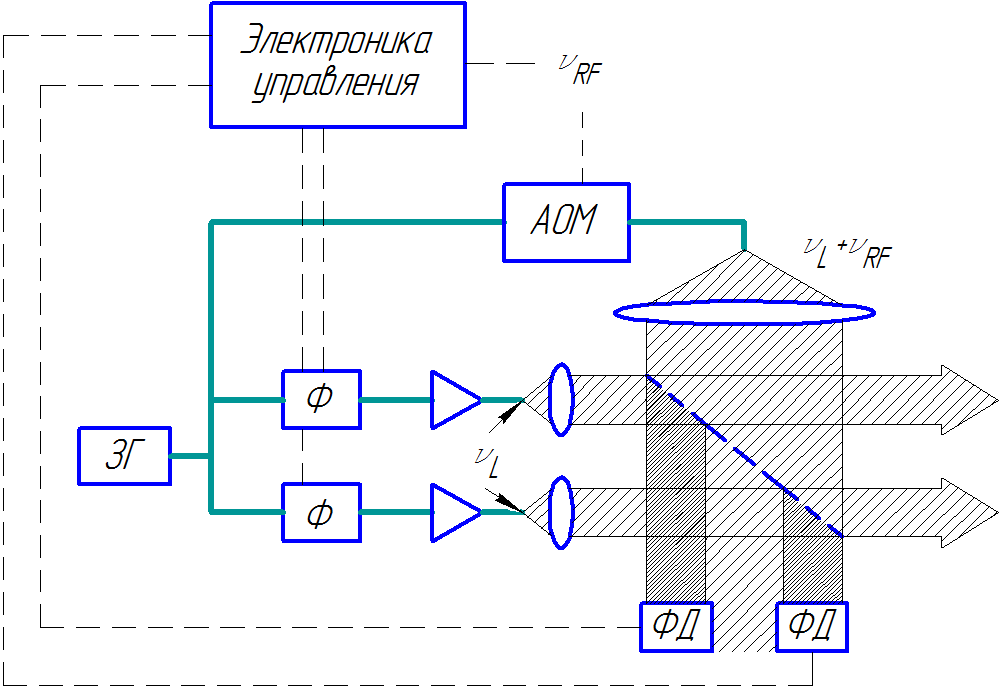
\includegraphics [scale=0.4] {locset_4}
  \caption{Установка гетеродинной блокировки фазы. Фаза каждого оптического канала блокируется относительно общего канала излучения со смещенной частотой (см. описание установки в~\cite{Locset20}).}
  \label{img:locset_4}
\end{figure}

Основные принципы техники гетеродинной активной регулировки фазы являются самыми интуитивнопонятными из всех  методов активного когерентного сложения. Показанная на рис.~\ref{img:locset_4} установка начинается слева с одиночного задающего генератора (ЗГ), выход которого расщепляется на три оптических канала. Излучение в двух каналах проходит через контроллеры фазы и впоследствии усиливаются. Усиленное излучение коллимируется и направляется вдоль пространственно разделенных оптических путей излучения и падет на общий частичный отражатель (сэмплер излучения). В каждом канале часть излучения отражается и падет на отдельный фотодетектор. Возвращаясь к ЗГ, остающееся излучение проходит через акустооптический модулятор, где оно подвергается радиочастотному (RF) смещению. Смещенное (модулированное) по частоте излучения коллимируется в одиночный пучок, больший, чем стыкованный выход усиленного излучения в каналах. Пучки излучения накладываются друг на друга и интерферируют на фотодетекторах. Каждый фотодетектор измеряет оптическое биение, которое содержит информацию о фазе каждого усиленного излучения, измеренного относительно общего опорного излучения~\cite{Locset20,Locset21,Locset22,Locset23,Locset24}. Контроллирующая электроника определяет разность фаз для каждого канала и минимизирует его величину~\cite{Locset20,Locset21,Locset22,Locset23,Locset24}. Разность фаз отдельных каналов, минимизированная  относительно опорного канала излучения, также будет минимизирована между отдельными каналами. Все это в идеале должно привести к когерентному сложению излучения отдельных каналов в системе.
\begin{figure} [ht]
  \center
  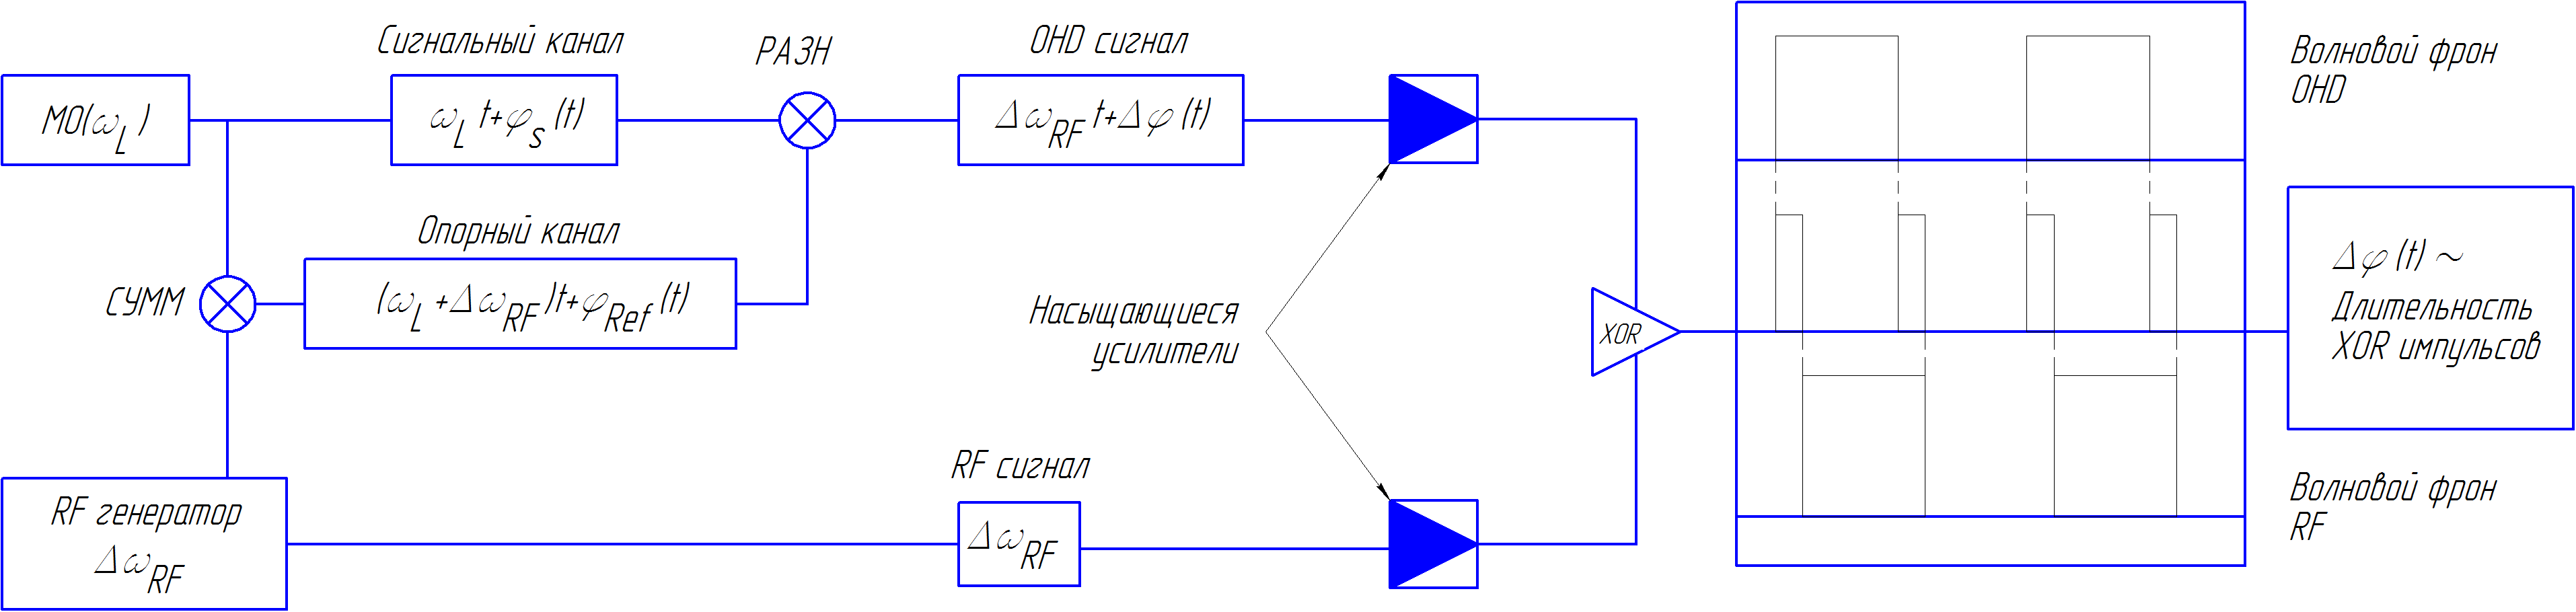
\includegraphics [scale=0.12] {locset_5}
  \caption{Схема контроля гетеродинного излучения. Цель состоит в том, чтобы минимизировать ширину импульса от <<исключающего ИЛИ (XOR)>> выхода цепи управления~\cite{Locset20}.}
  \label{img:locset_5}
\end{figure}
Основное действие цикла гетеродинного контроля излучения ---  минимизировать разность фаз между одиночными каналами излучения и смещенным по частоте опорным излучением ---  показано на рис.~\ref{img:locset_5}~\cite{Locset20}. Схема начинается слева с излучения с частотой $\omega_L$, сгенерированного ЗГ. Излучение расщепляется (см. рис.~\ref{img:locset_4}) на два пути. Верхний канал излучения имеет исходную частоту $\omega_L$ и фазовое состояние $\phi_s$, показанное на рис.~\ref{img:locset_5} как $\omega_L\cdot t+\phi(t)$. Второй канал подвергается сдвигу частоты $\Delta\omega_{RF}$ и поддерживает свое собственное уникальное оптическое фазовое состояние $\phi_{ref}$, показанное на рис.~\ref{img:locset_5} как $(\omega_L+\Delta\omega_{RF})\cdot t+\phi_{ref}(t)$. Когда излучение двух каналов смешиваются на фотодетекторе, он измеряет различие в частоте и фазе между двумя оптическими сигналами, представленное на рис.~\ref{img:locset_5} как $\Delta\omega_{RF}\cdot t+\Delta\phi(t)$, где $\Delta\phi(t)=\phi_{ref}(t)-\phi_s(t)$ и отмеченное как оптический гетеродиный (OHD) сигнал. Затем осциллирующий выход с фотодетектора с помощью насыщающегося электронного усилителя принимает форму пямоугольного TTL импульса. Прямоугольный OHD сигнал сравнивается с прямоугольным сигналом RF, ответственным за сдвиг частоты в опорном канале, через логическую схему <<исключающее ИЛИ>> (XOR). Когда сигналы OHD и RF находятся не в фазе, генерируется ряд импульсов с определенной шириной по времени. Эта ширина импульса пропорциональна оптической разности фаз между опорным излучением и исходным сигнальным излучением~\cite{Locset20}. Цепь, имеющая количественные данные о фазовой ошибке, применяет фазовую  коррекцию для предельного уменьшения ширины импульсов от схемы XOR и сведения их к  нулю или очень небольшой разности фаз между опорным и исходным излучением~\cite{Locset20}.

Описанная выше система имеет преимущество в относительно простой реализации при этом сохраняя высокую производительность с ошибками фазы RMS ниже $\lambda/80$ для комбинации из 2 каналов излучения~\cite{Locset23}. Недостатки системы проявляются при попытке масштабировать ее в сторону большего количества каналов. Например, при объединении 25 каналов излучения каждый из них должен быть хорошо выровнен отностительно опорного канала с минимальными смещениями, наклонами и другим ошибкам волнового фронта до падения на отдельные фотодетекторы. В техническом отношении выполнить установку крайне сложно даже в лабораторных условиях, не говоря уже об ее использовании в полевых условиях. Другая проблема связана со случаем потери опорного луча, например, из-за ошибки позиционирования или проблем в волоконно-оптическом тракте на пути опорного луча. В этом случае вся система теряет способность фазирования (захвата или запирания фазы, phase locking). В зависимости от приложения подобная сложность оперирования и выравнивания пучков излучения может быть нежелательной или даже недопустимой.

\subsubsection{Метод СПГС}

Основное ограничение описанного выше гетеродинного метода --- потребность в нескольких фотодетекторах (по одному на каждый канал) для блокировки фазы каждого канала массива относительно общего смещенного по частоте опорного канала. Для того, чтобы преодолеть это ограничение, были разработаны методы когерентного объединения излучения, которые используют только один фотодетектор. Один из наиболее многообещающих методов известен как \textit{Стохастический Параллельный метод Градиентного Спуска} (СПГС, SPGD)~\cite{Locset25,Locset26,Locset27,Locset28,Locset29,Locset30}.
\begin{figure} [ht]
  \center
  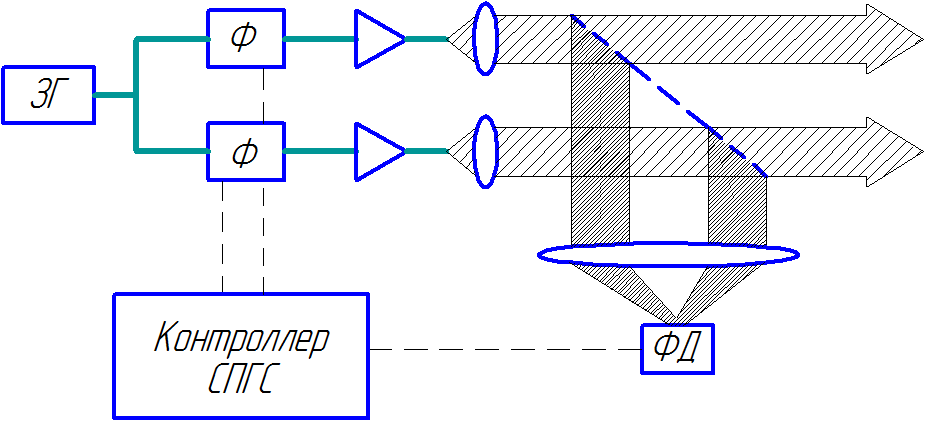
\includegraphics [scale=0.4] {locset_6}
  \caption{Стохастический параллельный метод градиентного спуска. СПГС для когерентно объединения N каналов излучения использует только один фотодетектор.}
  \label{img:locset_6}
\end{figure}
Метод СПГС когерентного объединения излучения, показанный на рис.~\ref{img:locset_6}, работает в точности как подразумевает его название. Стохастическое, или случайное, возмущение оптической фазы применяется параллельно к каждой контроллируемой фазе излучения в общей системе комбинации излучения. Алгоритм работает над минимизацией основанной на интенсивности метрики ошибки и минимизации этой метрики вдоль градиента ошибки с последующим когерентным объединением многоканального излучения на фотодетекторе. Когерентно объединяя стыкованный массив, показанный на рис.~\ref{img:locset_6} на фотодетекторе, каждое излучение будет в фазе с другим в выходной апертуре системы, справа от частичного отражателя (см. рис.~\ref{img:locset_6}).

Для реализации метода СПГС определяют вектор, который представляет оптическое фазовое состояние $\vec\phi_i$ массива $N$ оптических излучений~\cite{Locset31}
\begin{equation}\label{eq_locset_2.3}
  \vec\phi_i=\{\phi_1,\phi_2,\phi_3,...,\phi_N\}.
\end{equation}
Независимо от фазового состояния стыкованного массива контроллер СПГС применит случайное возмущение $\vec\rho$ к $\vec\phi_i$
\begin{equation}\label{eq_locset_2.4}
  \hat\phi=\vec\phi_i+\vec\rho.
\end{equation}
То, как случайное фазовое возмущение $\vec\rho$ выбирается, является главным вопросом при реализации метода СПГС в системе сложения излучения. В самой простой реализации $\vec\rho$ должен предопределить постоянную величину фазового шага, который будет применен к каждому фазовому модулятору в системе комбинации излучения, оставляя (опуская) только знак указанного шага для каждого элемента с контроллируемой фазой, к стохастическому определению алгоритма СПГС~\cite{Locset31}. После указанного случайного фазового возмущения скалярное значение ошибки $\epsilon$ определяется путем вычисления различия интенсивности, измереной для обоих фазовых состояний $\vec\phi_i$ и $\hat\phi$
\begin{equation}\label{eq_locset_2.5}
  \epsilon=I(\hat\phi)-I(\vec\phi),
\end{equation}
где $I(\vec\phi_j)$ --- интенсивность на фотодетекторе объединенного излучения для некоторого фазового состояния $\vec\phi_j$ массива. Это значение ошибки $\epsilon$ умножается на другое скалярное значение $\mu$, которое соответствует параметрам цикла контроля  СПГС, таким как электронное усиление и работает ли система СПГС над максимизацией или минимизацией интенсивности на фотодетекторе~\cite{Locset25}. При максимизации интенсивности $\mu$ выбирается положительным. При минимизации интенсивностм объединенного излучения $\mu$ выбирается отрицательным. Затем величина $\mu\cdot\epsilon$ умножается на стохастически выбранное фазовое возмущение $\vec\rho$, чтобы определить необходимую величину фазовой коррекции
\begin{equation}\label{eq_locset_2.6}
  \Delta\vec\phi=\pm\mu\cdot\epsilon\cdot\vec\rho
\end{equation}
и применить ее к исходному невозмущенному состоянию фазы массива $\vec\phi_i$, а также сгенерировать скоррекированное фазовое состояние $\vec\phi_{i+1}$
\begin{equation}\label{eq_locset_2.7}
  \vec\phi_{i+1}=\vec\phi_i+\Delta\vec\phi.
\end{equation}
При стремлении к когерентному объединению излучения исправленное фазовое состояние $\vec\phi_{i+1}$ не обязательно является оптимальным фазовым состоянием массива, но, если алгоритм управления реализуется правильно, это будет шаг в правильном направление (то есть больше, или по крайней мере одинаковое, оптимальное фазовое состояние, чем $\vec\phi_i$). Затем алгоритм повторяется пока система СПГС не сходится к оптимальной комбинации излучения на фотодетекторе~\cite{Locset26,Locset28} (см. рис.~\ref{img:locset_7}).
\begin{figure} [ht]
  \center
  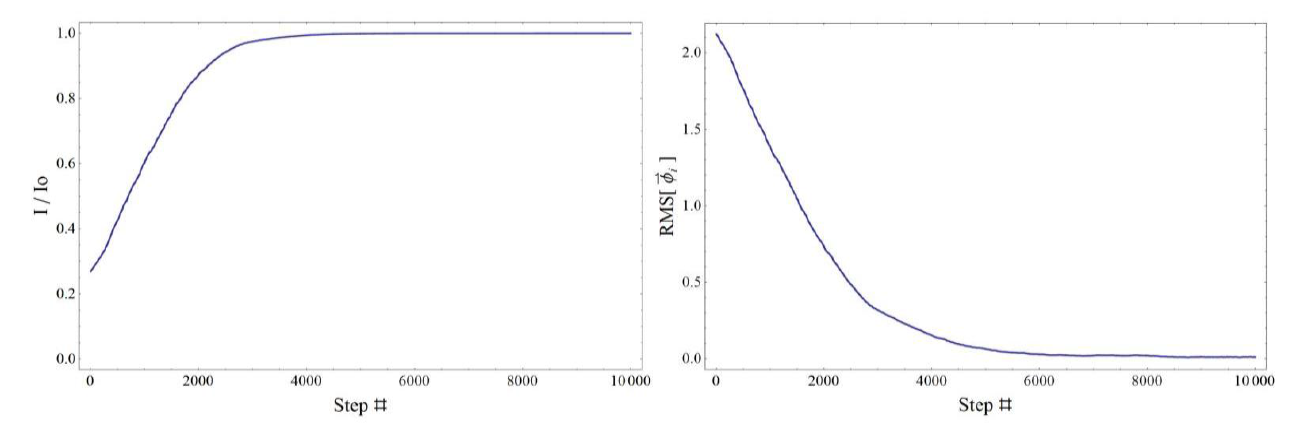
\includegraphics [scale=0.4] {locset_7}
  \caption{Результаты числового моделирования СПГС. Слева: Нормированная пиковая интенсивность, измеренная на фотодетекторе на рис.~\ref{img:locset_6} для 10-канальной системы когерентного объединения излучения. Справа: значение RMS, вычисленное из фазовых состояний 10 когерентно объединенных каналов излучения. Оба: Для простоты все излучения идельно укладывалось на фотодетекторе (то есть это не стыкованный массив)~\cite{Locset_pulford}.}
  \label{img:locset_7}
\end{figure}
На рис.~\ref{img:locset_7} приведены результаты числового моделирования СПГС~\cite{Locset_pulford}. При проведении моделирования предполагалось наличие 10 идеально перекрытых пучков излучения (не стыкованных), абсолютно идентичных по всем характеристикам со случайно выбранным  фазовым состоянием. На рис.~\ref{img:locset_7} слева показана пиковая интенсивность объединенного излучения, измереного на фотодетекторе (см. рис.~\ref{img:locset_6}), вычисленная после применения  фазовой коррекции и нормированная на теоретический максимум $I_0$ для каждой из 10 000 итераций алгоритма СПГС. Важно отметить, что на рис.~\ref{img:locset_7} не включены колебания интенсивности, следующие из стохастических фазовых возмущений, необходимых для определения величины ошибки $\epsilon$. На рис.~\ref{img:locset_7} справа приведено расчетное значение RMS фазы  объединенного излучения для каждой итерации алгоритма СПГС. Отметим, что, поскольку пиковая интенсивность объединенного излучения оптимизирована --- поведение RMS фазы объединенного излучения стремится к нулю. Это означает, что, максимизируя оптическую интенсивность объединенного излучения, система также минимизирует оптическую разность фаз между 10 пучками излучениями. СПГС --- превосходный метод оптической блокировки фазы, поскольку является относительно легким в реализации и продемонстрировал производительность блокировки фазы $\lambda/30$ на канал в 48 канальной мультидетекторной системе (раздельные СПГС контроллеры для каждого стыкованного элемента массива)~\cite{Locset32}. Однако, система СПГС все же не лишена проблем. Наиболее существенной является отношение между пропускной способностью цикла СПГС контроля и числом объединяемых каналов излучения. Хотя это никогда явно не отмечалось, но это не трудно понять из литературы, что пропускная способность цикла контроля $BW_{SPGD}$ обратно пропорциональна числу параметров $N$, которые цикл контроля должен исправлять~\cite{Locset28}
\begin{equation}\label{eq_locset_2.8}
  BW_{SPGD}\approx\frac{1}{N}.
\end{equation}
Поэтому, при увеличении общего числа каналов, пропускная способность СПГС контроля также уменьшается. В литературе часто сообщается об уровнях выборки в 100 кГц. Поэтому, если у системы сложения излучения есть 10 каналов, системная пропускная способность уменьшается до 10 кГц. При 100 каналов пропускная способность снижается до 1 кГц. В ряде приложений эти компромиссы могут быть приемлемыми. Если же требуется более высокая пропускная способность, тогда придется реализовывать другой метод блокировки фазы. Также стоит отметить, что, поскольку система является стохастической и ее действие базируется на интенсивности, к объединенному  излучению может быть применено любое число коррекций [26]. С другой стороны, число исправленных фазовых аберраций в каждом канале увеличивает число корректируемых параметров в цикле СПГС контроля. Это увеличение  понижает системную пропускную способность СПГС (см. уравнение~\eqref{eq_locset_2.8}). Однако, в свою очередь это может увеличить производительность сложения излучения в турбулентной среде~\cite{Locset26}.

\subsubsection{Метод LOCSET}

Как и метод СПГС техника \textit{Блокировки Оптической Когерентности через Однодетекторное Теггирование Электронной частоты} (Locking of Optical Coherence via Single-detector Electronic-frequency Tagging, LOCSET), показанная на рис.~\ref{img:locset_8}, использует одиночный фотодетектор для генерации сигнала устранения ошибки и достижения оптимальной фазовой блокировки. В отличие от метода СПГС LOCSET не стохастический. Вместо этого, используя метод RF-демодуляции, электроника LOCSET способна к независимому определению сигнала ошибки пропорционального оптической разности фаз в каждом канале излучения и измеренного относительно любого излучения в более широкой системе сложения излучения~\cite{Locset33,Locset34,Locset35,Locset36,Locset37,Locset38,Locset39,Locset40,Locset41,Locset42,Locset43}.
\begin{figure} [ht]
  \center
  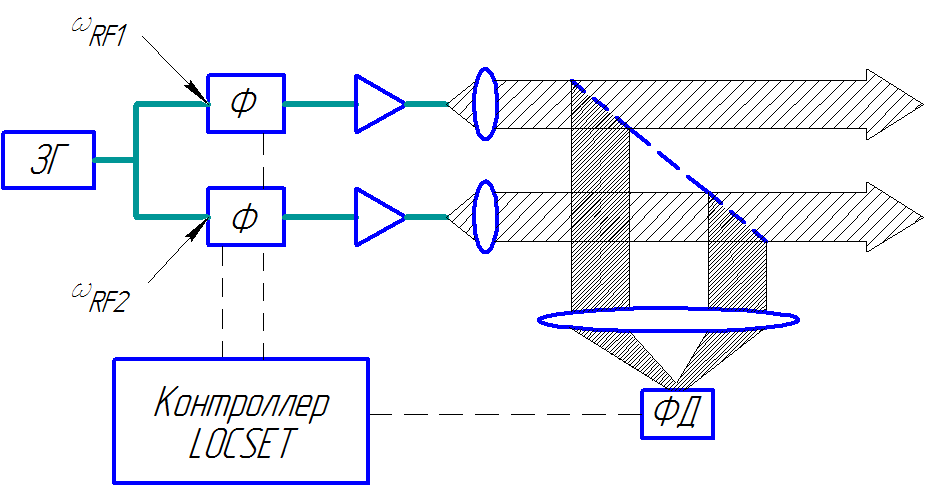
\includegraphics [scale=0.4] {locset_8}
  \caption{Метод блокировки оптической когерентности через однодетекторное теггирование электронной частоты (LOCSET) для когерентного объединения излучения. LOCSET способен к определению оптической разности фаз одиночного пучка излучения,  измеренного относительно остальных пучков в системе когерентного объединения излучения.}
  \label{img:locset_8}
\end{figure}
Метод блокировки фазы LOCSET, показанный на рис.~\ref{img:locset_8}, напоминает метод СПГС. Система начинается с совместно используемого задающего генератора, выход которого разделяется на $N$ каналов (на рис.~\ref{img:locset_8} $N = 2$). Каждый из $N$ пучков проходит через фазовый модулятор, предоставляющий собой электронику контроля за LOCSET с возможностью коррекции фазы в каждом канале системы и когерентного объединения излучения на фотодетекторе. Каждый из $N$ пучков усиливается, коллимируется и выходит через выходную апертуру системы (на рис.~\ref{img:locset_8} показана выходная апертура сразу после частичного отражателя). Часть излучения от частичного отражателя перекрывается и интерферирует на одиночном фотодетекторе, который предоставляет сигнал в цепь контроля за LOCSET. Для того, чтобы достигнуть оптимального сложения излучения, каждый из $N$ каналов <<тегируется>> с малым амплитудным размытием фазы определенной уникальной RF частотой. Затем фазовые размытия измеряются на фотодетекторе как биение интенсивности, которое содержит фазовую информацию, необходимую для когерентного объединения излучения~\cite{Locset33,Locset34,Locset35,Locset36,Locset37,Locset38,Locset39,Locset40,Locset41,Locset42,Locset43}.

Есть две конфигурации метода блокировки фазы LOCSET: \textit{самоссылаемая}~\cite{Locset35,Locset37,Locset41,Locset42} и \textit{самосинхронная}~\cite{Locset33,Locset34,Locset43}. Выражение для сигнала ошибки в самоссылаемой конфигурации  для одиночного канала ($x$-ый канал) $S_{SR_x}$, который управляет процессом принятия решений LOCSET, определяется следующим образом~\cite{Locset_pulford}:
\begin{equation}\label{eq_locset_2.9}
  S_{SR_x}=R_{PD}\cdot P_x^{1/2}\cdot J_1(\beta_x)\left(P_u^{1/2}\sin(\phi_u-\phi_x)+\frac{1}{2}\sum_{j=1, j\neq x}^{N-1}P_j^{1/2}\cdot J_0(\beta_j)\cdot\sin(\phi_j-\phi_x)\right).
\end{equation}
Здесь $S_{SR_x}$ --- самоссылаемый электронный сигнал ошибки для $x$-го модулированного по фазе канала, $R_{PD}$ --- чувствительность фотодетектора, $P_x$ -- оптическая мощность интересуемого $x$-го модулированного по фазе канала (канал, который корректирует система) и $\beta_x$ --- амплитуда уникальной RF модуляции фазы, примененной к $x$-ому каналу. Другими важными параметрами в уравнении~\eqref{eq_locset_2.9} являются $P_u$ --- оптическая мощность в немодулируемом опорном канале излучения (если присутствует), $P_j$ --- оптическая мощность $j$-го модулированном по фазе канале, где $j\neq x$ и $\phi_u, \phi_x, \phi_j$ --- оптические фазовые состояния немодулируемого опорного излучения, $x$-го модулированного по фазе канала излучения и $j$-го модулированного излучения соответственно. Отметим, что сигнал ошибки пропорционален синусу разности фаз между немодулируемым опорным излучением и интересующим $x$-ым модулированным по фазе излучением $\sin(\phi_u-\phi_x)$, а также сумме синуса разности фаз между $x$-ым модулированным по фазе излучение и оставшимися $j$ каналами, модулированными по фазе
$$
  \sum_{j=1, j\neq x}^{N-1}P_j^{1/2}\cdot J_0(\beta_j)\cdot\sin(\phi_j-\phi_x).
$$
Это указывает на то, что независимо сгенерированные сигналы ошибки LOCSET для каждого из модулированных по фазе каналов пропорциональны оптической разности фаз между каждым отдельным каналом, измеренным относительно всех других каналов излучения в системе когерентного объединения.

Поскольку фазовое поведение каждого пучка известно относительно всех других каналов излучений в системе, в немодулированном опорном излучении больше нет необходимости. Это очевидно, если устанавить оптическую мощность немодулированного опорного излучения в уравнении~\eqref{eq_locset_2.9} в нуль и получить выражение для самосинхронного сигнала ошибки LOCSET $S_{SS_x}$~\cite{Locset33,Locset34,Locset43}
\begin{equation}\label{eq_locset_2.10}
  S_{SS_x}=R_{PD}\cdot P_x^{1/2}\cdot J_1(\beta_x)\cdot\frac{1}{2}\sum_{j=1, j\neq x}^{N-1}P_j^{1/2}J_0(\beta_j)\sin(\phi_j-\phi_x).
\end{equation}
Причина того, что LOCSET способен оперировать без опорного излучения, состоит в том, что метод измеряет относительную фазовую ошибку одиночного излучения относительно любого излучения в системе. Поскольку фазовая информация данного излучения известна относительно всех других, необходимости в опорном излучении нет, поскольку оно является лишь элементом большего когерентно объединенного излучения.

Преимущество LOCSET по сравнению с гетеродинным методом и методами блокировки фазы СПГС состоит в его работе с одиночным детектором. Так как каждый канал цикла контроля работают независимо от остальных, пропускная способность цикла контроля независит от числа управляемых по фазе каналов в системе~\cite{Locset33}. В~\cite{Locset_pulford} продемонстрирована LOCSET блокировка фазы для 32 когерентно объединенных каналов излучения, тем самым двое увеличен предыдущий рекорд LOCSET равный 16, с высоким качеством сложения излучения (RMS $\lambda/71$ для 32 каналов).

\subsubsection{Ограничения активного метода КОИ со стыкованной апертурой}

Вышеупомянутые результаты указывают на то, что активный метод КОИ массива на базе ЗГ-У может быть успешно применен для масштабирования больших массивов и высоких объединенных мощностях. Несмотря на многообещающие результаты, метод имеет ряда проблем, которые ограничивают его производительность и удобство практического использования.

Некоторые из недостатков очевидны --- требование нескольких изоляторов высокой мощности, сложность системы, требования точного соответствия длин пути усилителей, а также большой размер полученной системы. Сложность системы исходит из необходимости разработки и применения сложных механизмов активного управления, которые используют чувствительные схемы гетеродинного обнаружения, несколько обратных связей и быстрые алгоритмы обработки сигналов.

Более серьезное ограничение в масштабировании мощности возникает из требования ультраузкой ширины спектральной линии у задающего генератора. Источники с узкой шириной спектральной линии гарантируют, что длина когерентности больше, чем разница в длине оптического пути в усилителях. Это обеспечивает генерацию биений частоты, требуемых для процесса активной регулировки фазы. Это требование снижает порог SBS, ограничивающий выходные мощности от каждого усилительного каскада. Подавление SBS в таких лазерных массивах --- активная тема исследований, и многочастотные подходы являются наиболее многообещающими~\cite{Jain118, Jain124}.

Другой недостаток, характерный для всех приведенных реализаций, связан с проблемой коэффициента заполнения, свойственной массивам со стыкованными апертурами. В дальней зоне качество такого излучения сильно ухудшается, и существенная мощность теряется на <<хвостах>>. Например, в~\cite{Jain117} Ю и др. объединяли излучение с суммарной мощностью в 4 кВт в массиве стыкованных апертур, у которого только 58 \% мощности было в центре, в то время как 42 \% были потеряны на <<хвостах>> в дальней зоне.

Активное КОИ с заполненной апертурой --- область повышенного интереса исследований. Предложено несколько методов, включая использование волноводов с обращением изображения~\cite{Jain125}, когерентное поляризационное объединение излучения~\cite{Jain126}, а также использование поверхностных дифракционных оптических элементов (ДОЭ, DOE)~\cite{Jain120, Jain127,Jain128,Jain129,Jain130}. Из всего описанного использование ДОЭ для объединения излучения в ближней зоне   является наиболее интересным в настоящее время и будет более подробно описано ниже. Отметим, что, хотя методы с заполненной апертурой решают проблему <<хвостов>> в дальней зоне, при это теряется возможность регулировки излучения и коррекции атмосферных искажений.

\subsubsection{Активное КОИ с ДОЭ}

Для перекрытия каждого пучок излучения от массива оптических усилителей как в ближней, так и в дальней зоне, Викхем (Wickham) и др.~\cite{Jain128} предложили добавить на выходе дифракционный оптический элемент (см. рис.~\ref{img:jain_4_10}). Используя этот метод, массив оптических усилителей из 5 элементов при низких уровнях мощности в десятки миливатт был сфазирован с эффективностью объединения 91,4 \% (процент мощности в объединенном пятне в дальней зоне относительно суммарной мощности на ДОЭ) и $M^2$=1,04. В~\cite{Jain129} Редмонд и др. используя поверхностный ДОЭ объединили массив из пяти 500~Вт усилителей с эффективностью 79 \% и 1,93 кВт в объединенном пучке излучения с $M^2$=1,1.
\begin{figure} [ht]
  \center
  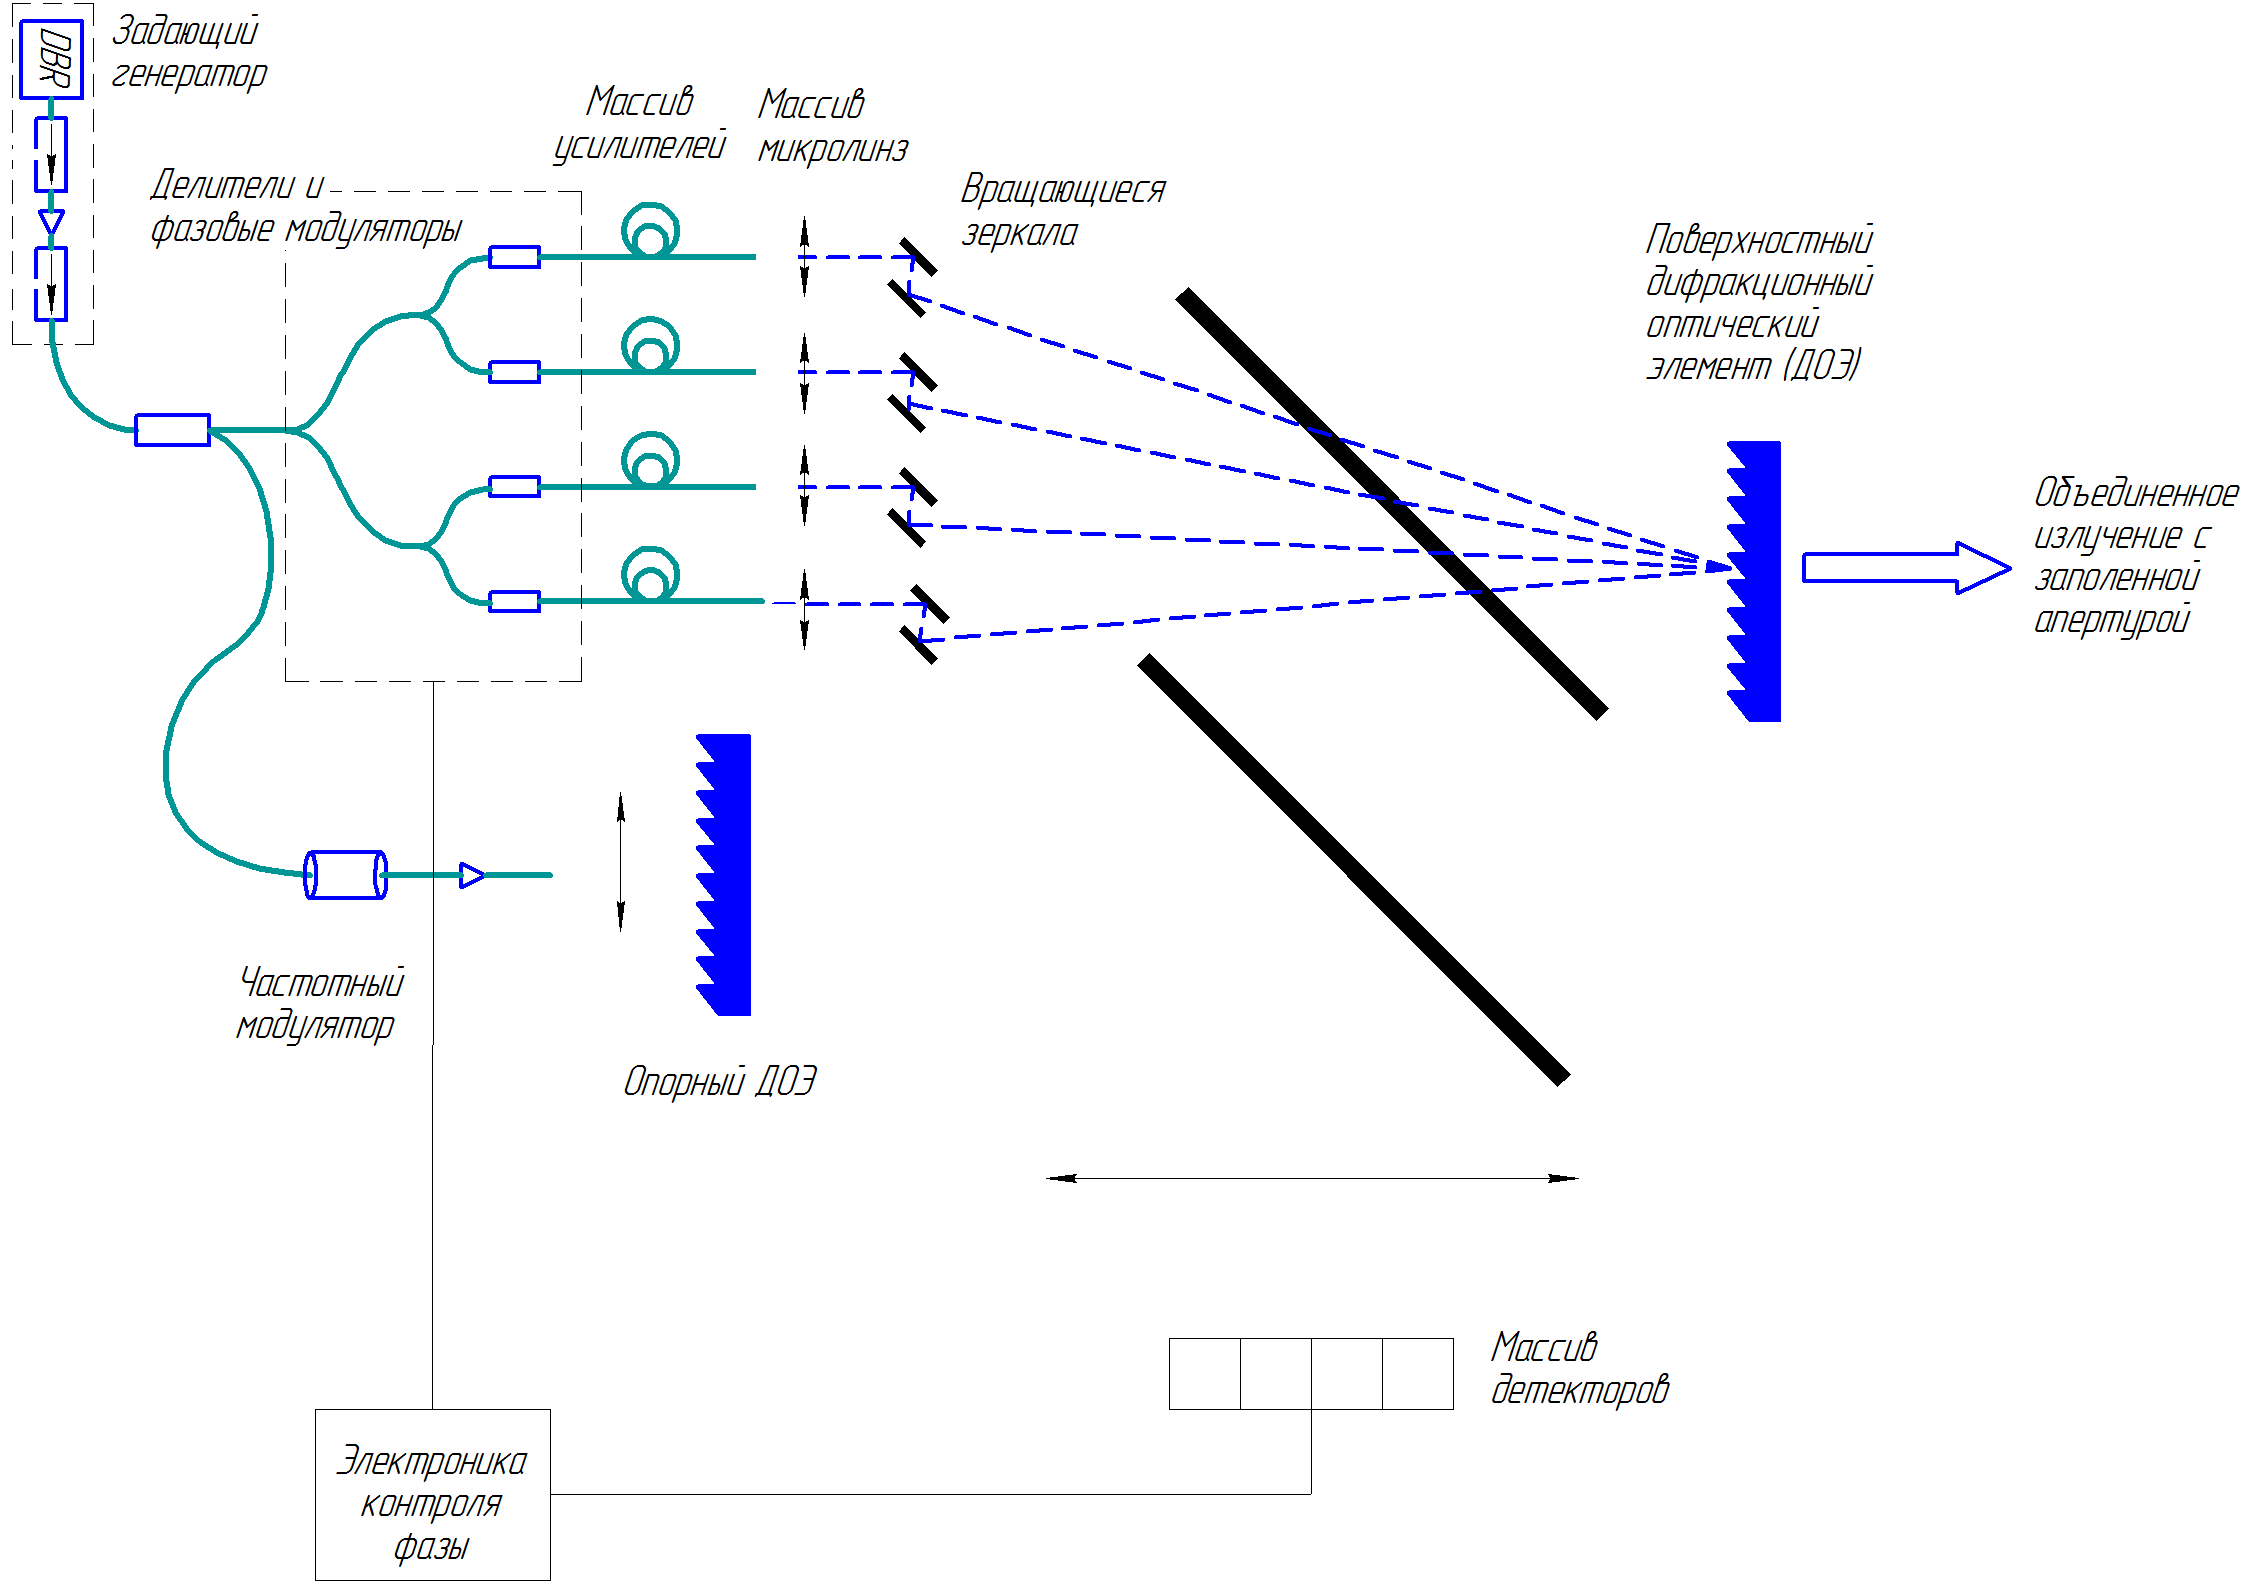
\includegraphics [scale=0.15] {jain_4_10}
  \caption{Схема активной системы КОИ с заполненной апертурой на базе ЗГ-У с использованием ДОЭ.}
  \label{img:jain_4_10}
\end{figure}
Этот метод был расширен до 2D массива 3x5 усилителей путем мультиплексирования ортогональных поверхностных профилей на одном ДОЭ. Таким образом, были объединены 15 усилителей с эффективностью 70 \% и мощностью 0,6 кВт~\cite{Jain130}.
\begin{table} [htbp]
  \centering
  \parbox{16cm}{\caption{{Использованные волоконно-оптические элементы при активном когерентном объединении излучения.}}
  \label{tbl_nrl_5}}
  \begin{center}
  \begin{tabular}{ | p{6cm} | p{9cm} |}
  \hline
  \hline
  Тип & Характеристики \\
  \hline
  \hline
    Акустооптический модулятор & Минимальная инерционность (быстрый отклик на входящий сигнал); возможность интеграции с волоконными элементами; высокая точность модуляции \\
  \hline
    Фазовый модулятор &  Минимальная инерционность (быстрый отклик на входящий сигнал); возможность интеграции с волоконными элементами; высокая точность коррекции\\
  \hline
    Объемные зеркало &  Частичное отражение; отсутствие искажений волнового фронта; высокая однородность и равномерность покрытия\\
  \hline
    Коллиматор &  Возможность интеграции с волоконными элементами\\
  \hline
    Дифракционный оптический элемент &  Высокая точность позиционирования; высокая точность исполнения дифракционной структуры элемента \\
  \hline
  \end{tabular}
\end{center}
\end{table}

\subsection{Пассивное когерентное объединение излучения}

Методы пассивного когерентного объединения излучения позволяют объединить массив лазерных источников без какой-либо активной обратной связи и электронных регулировок фаз. Простота архитектуры объединения делает пассивные методы очень привлекательными. Торри Вагнер из Научно-исследовательской лаборатории ВВС США (AFRL) назвал их <<святым Граалем>> масштабирования мощности волоконных лазеров~\cite{Jain131}. За последнее время были предложены несколько методов пассивного КОИ. В большинстве из них для получения самоорганизованного фазирования лазерного массива используется некоторая конфигурация общего резонатора. Эти подходы могут быть разделены на \textit{интерференционные} и \textit{пространственные методы фильтрации}. Пространственные методы фильтрации могут также быть классифицированы как  методы с  резонатором Тальбо, собственным Фурье-резонатором и методы с кольцевым резонатором.

Кроме упомянутых выше методов для пассивного фазирования лазерных массивов существует еще ряд менее популярных методов. Один из них основан на затухании связи оптических полей излучения близко расположенных эмиттеров. При затухании связи пучки излучения отдельных эмиттеров частично пространственно накладываются на пучки излучения соседних эмиттеров, таким образом появляется связь в поперечном направлении. Минден и др.~\cite{Jain132} продемонстрировали когерентное излучение нескольких волоконных лазеров, разработав плотно упакованный жгут оптических волокон с затухающей связью выходящего излучения. Жгут был сколот в самой узкой части, формирующей выходную апертуру и каплер (см. рис.~\ref{img:jain_4_11}). Было продемонстрировано когерентное действие из-за сильно затухающей связи вдоль длинного участка взаимодействия (15 м). Эффективность когерентного сложения жгута легированного Yb волокна с 7 сердцевинами составила 65 \%~\cite{Jain133}. Затухающая связь сама по себе недостаточно эффективна для когерентной блокировки больших массивов, так как взаимодействие ограничивается соседними элементами. Однако, его можно эффективно использовать в комбинации с другими методами.

\begin{figure} [ht]
  \center
  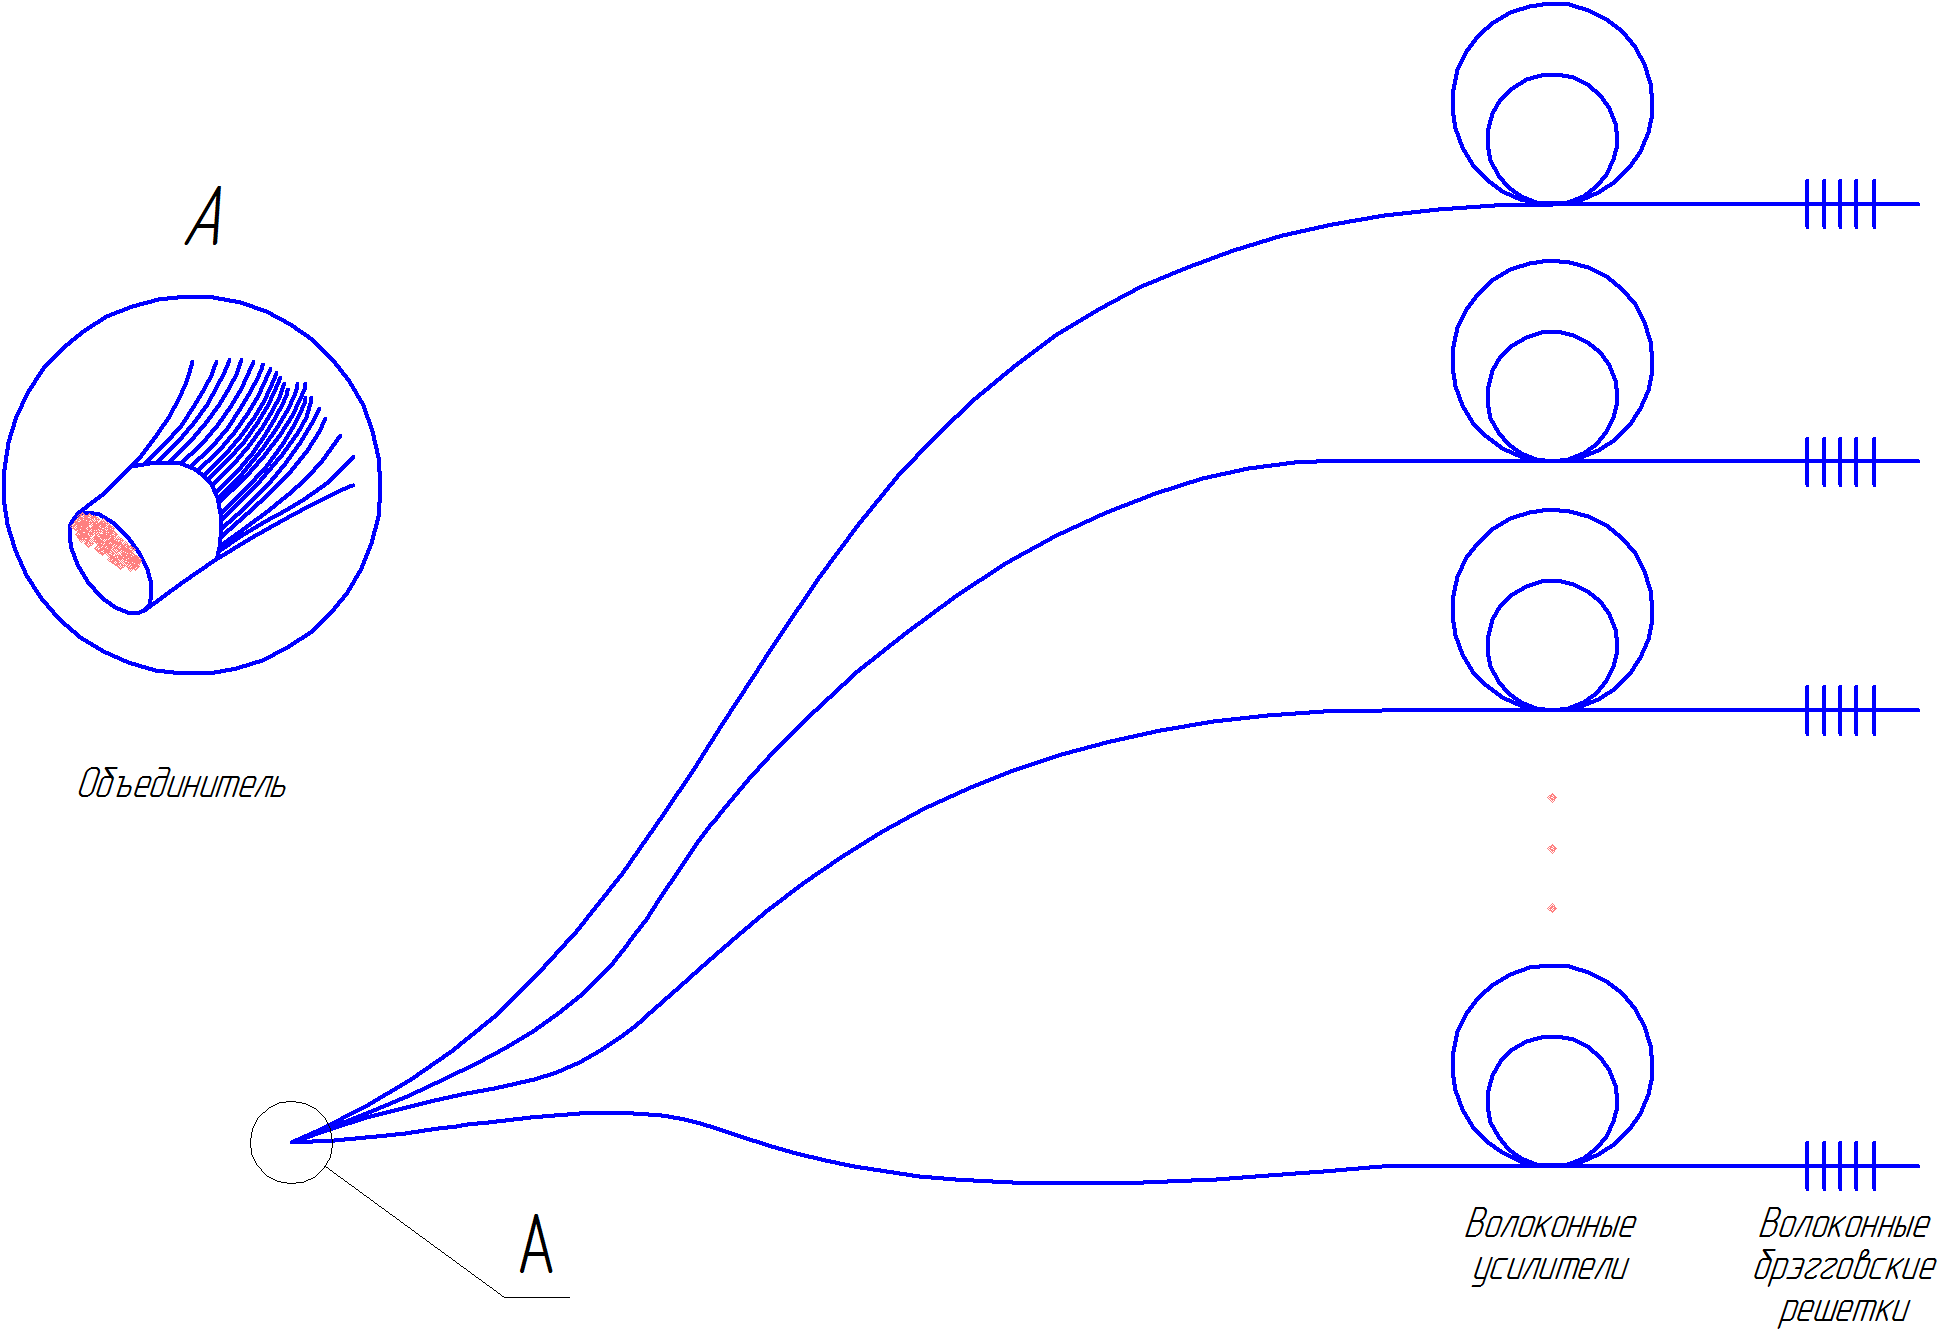
\includegraphics [scale=0.2] {jain_4_11}
  \caption{Схема с затухающей связью, использованная Минденом и др.}
  \label{img:jain_4_11}
\end{figure}

Следует отметить, что описанные методы КОИ были продемонстрированы для небольших массивов и низких уровней мощности. Целью большинства исследований в данной области является получение простого, устойчивого и масштабируемого подхода. Рядом авторов были предприняты попытки теоретически проанализировать физические механизмы, ответственные за когерентную связь в этих методах [ссылки на эти статьи]. Обсуждения ниже будут ограничены базовым описанием этих методов.

% \subsection{Интерференционные методы}

Интерференционные методы пассивного когерентного объединения излучения волоконных лазеров обычно включают размещение отдельных лазеров в интерферометре Майкельсона, обобщенного для использования более двух <<плечей>>~\cite{Jain134}. Интерферометр может быть реализован на волоконных разветвителях или объемных делителях пучков излучения как показано на рис.~\ref{img:jain_4_12} для двух элементов усиления. Масштабирование для больших массивов было достигнуто при использовании древовидной архитектуры или ветвителями NxN (см. рис.~\ref{img:jain_4_13}). Для пассивного КОИ также предложено и теоретически проанализировано использование дифракционных объединителей Nx1. Однако было выполнено лишь несколько экспериментов при малой мощности и для малого размера массива~\cite{Jain134, Jain135}.

\begin{figure} [ht]
  \center
  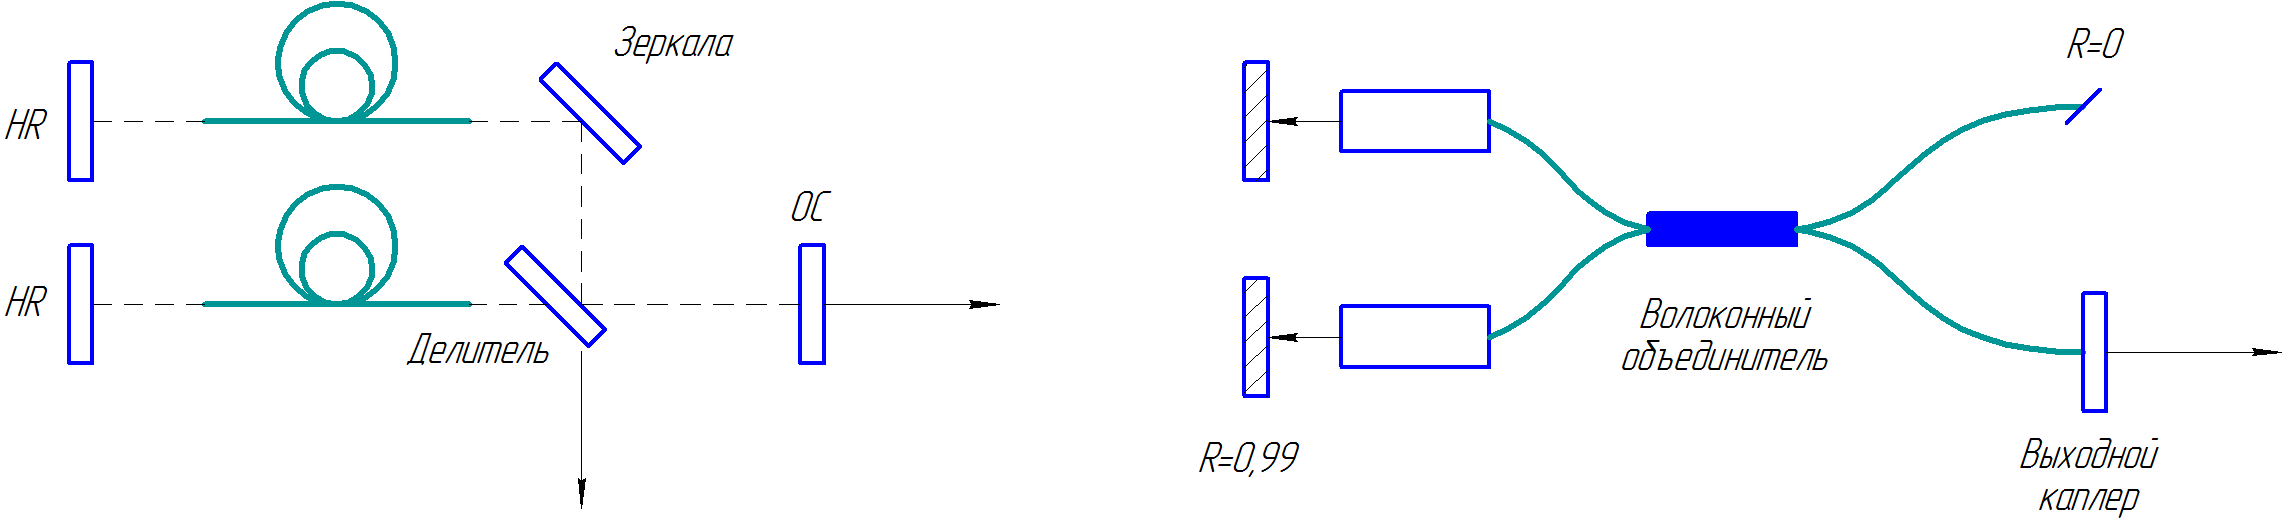
\includegraphics [scale=0.2] {jain_4_12}
  \caption{Пассивный КОИ с интерферометром Майкельсона в свободном пространстве (слева) и цельноволоконный (справа).}
  \label{img:jain_4_12}
\end{figure}


\begin{figure} [ht]
  \center
  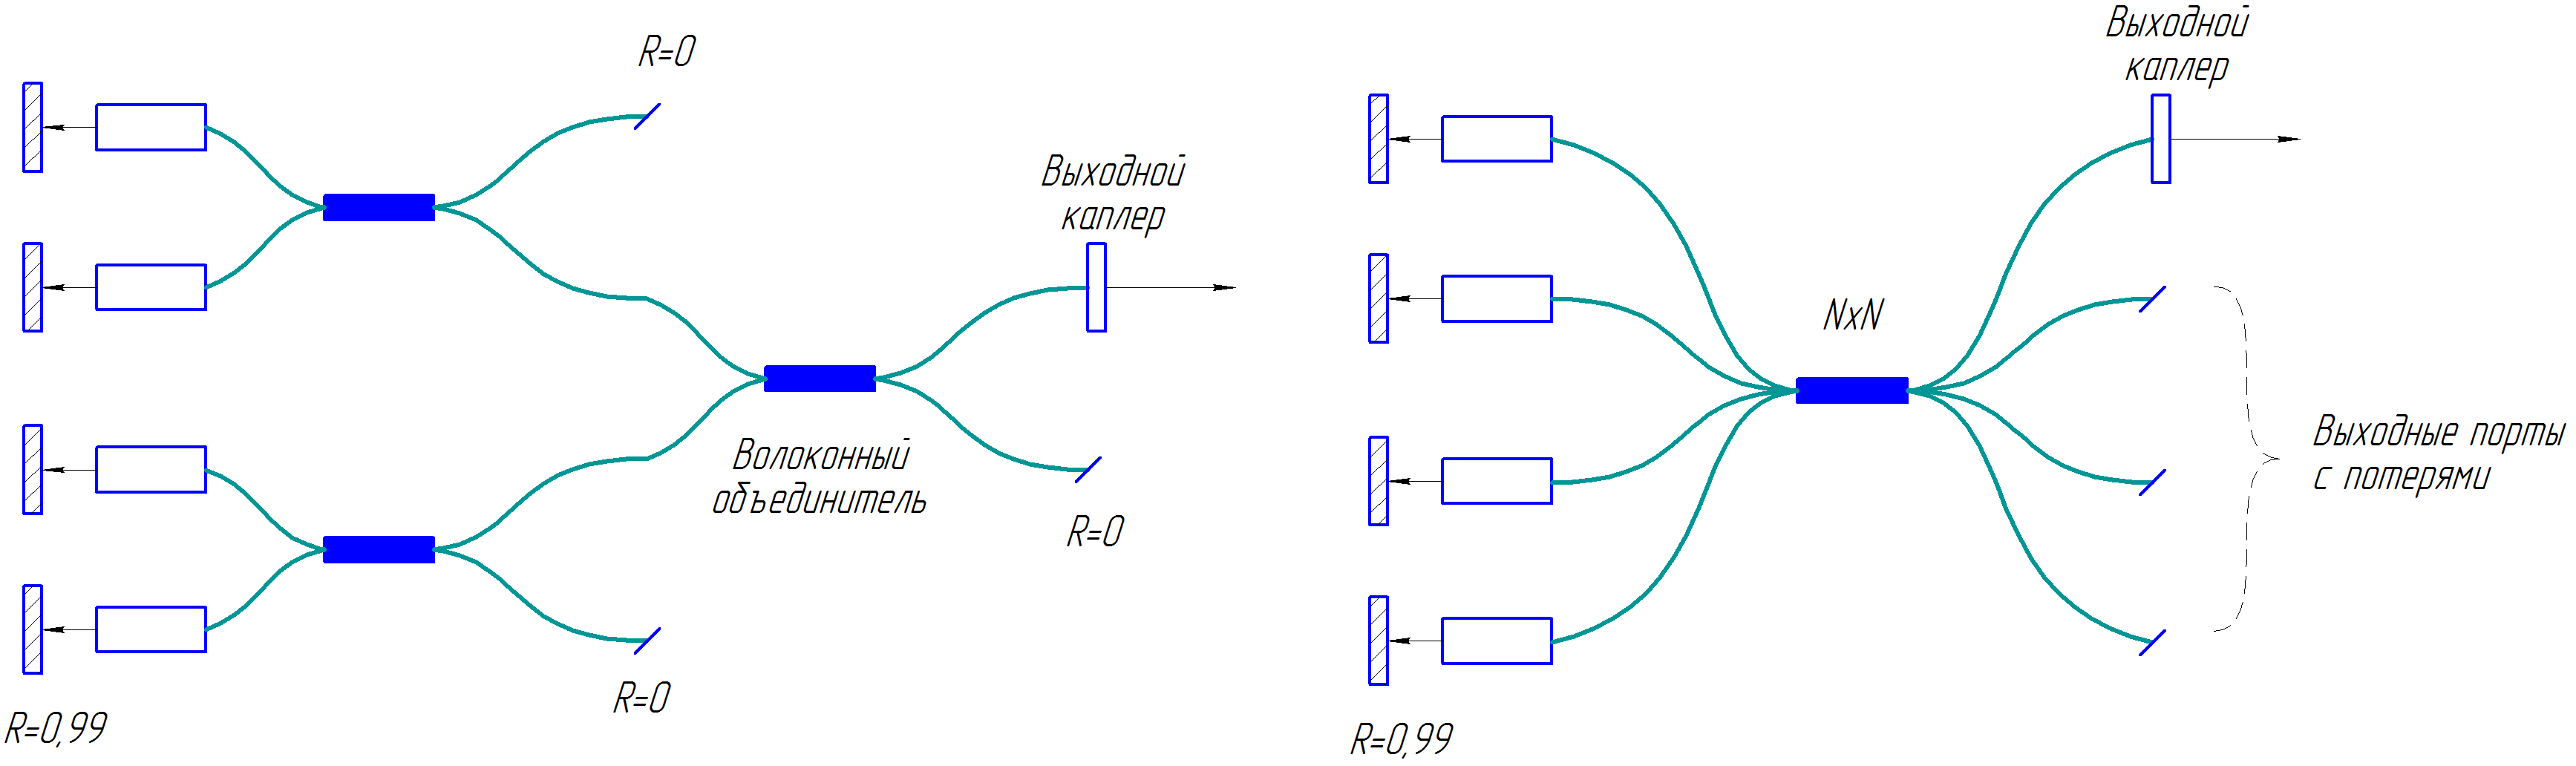
\includegraphics [scale=0.14] {jain_4_13}
  \caption{Масштабирования размера массива с помощью ветвителя 2x2 с древовидной архитектурой (слева) и ветвителей NxN (справа).}
  \label{img:jain_4_13}
\end{figure}

Рассмотрим самый простой случай объединения двух волоконных лазеров в интерферометре Майкельсона (рис.~\ref{img:jain_4_12}). Выходы двух сред усиления смешиваются в делителе пучка излучения, который разделяет две супермоды общего резонатора. Помещая элемент обратной связи только в одно плечо можно обеспечить приоритетную обратная связь только для одной из супермод, в то время как излучение в другом плече полностью затухает. Поэтому две среды усиления находятся в общем резонаторе с общей обратной связью, что гарантирует взаимокогерентное действие. На интуитивном уровне когерентное действие объясняется, если рассматривать его в обратную по времени сторону. Пучок излучения падающий на делитель 50:50 (см. рис.~\ref{img:jain_4_14}a) будет разделен на два пучка с равными интенсивностями, взаимно когерентными и с уникальным фазовым соотношением. Если инвертировать направление этих пучков излучения (см. рис.~\ref{img:jain_4_14}b), то два когерентных пучка с равной интенсивностью и тем же самым фазовым соотношением этим делителем будут объединены в один пучок излучения.

\begin{figure} [ht]
  \center
  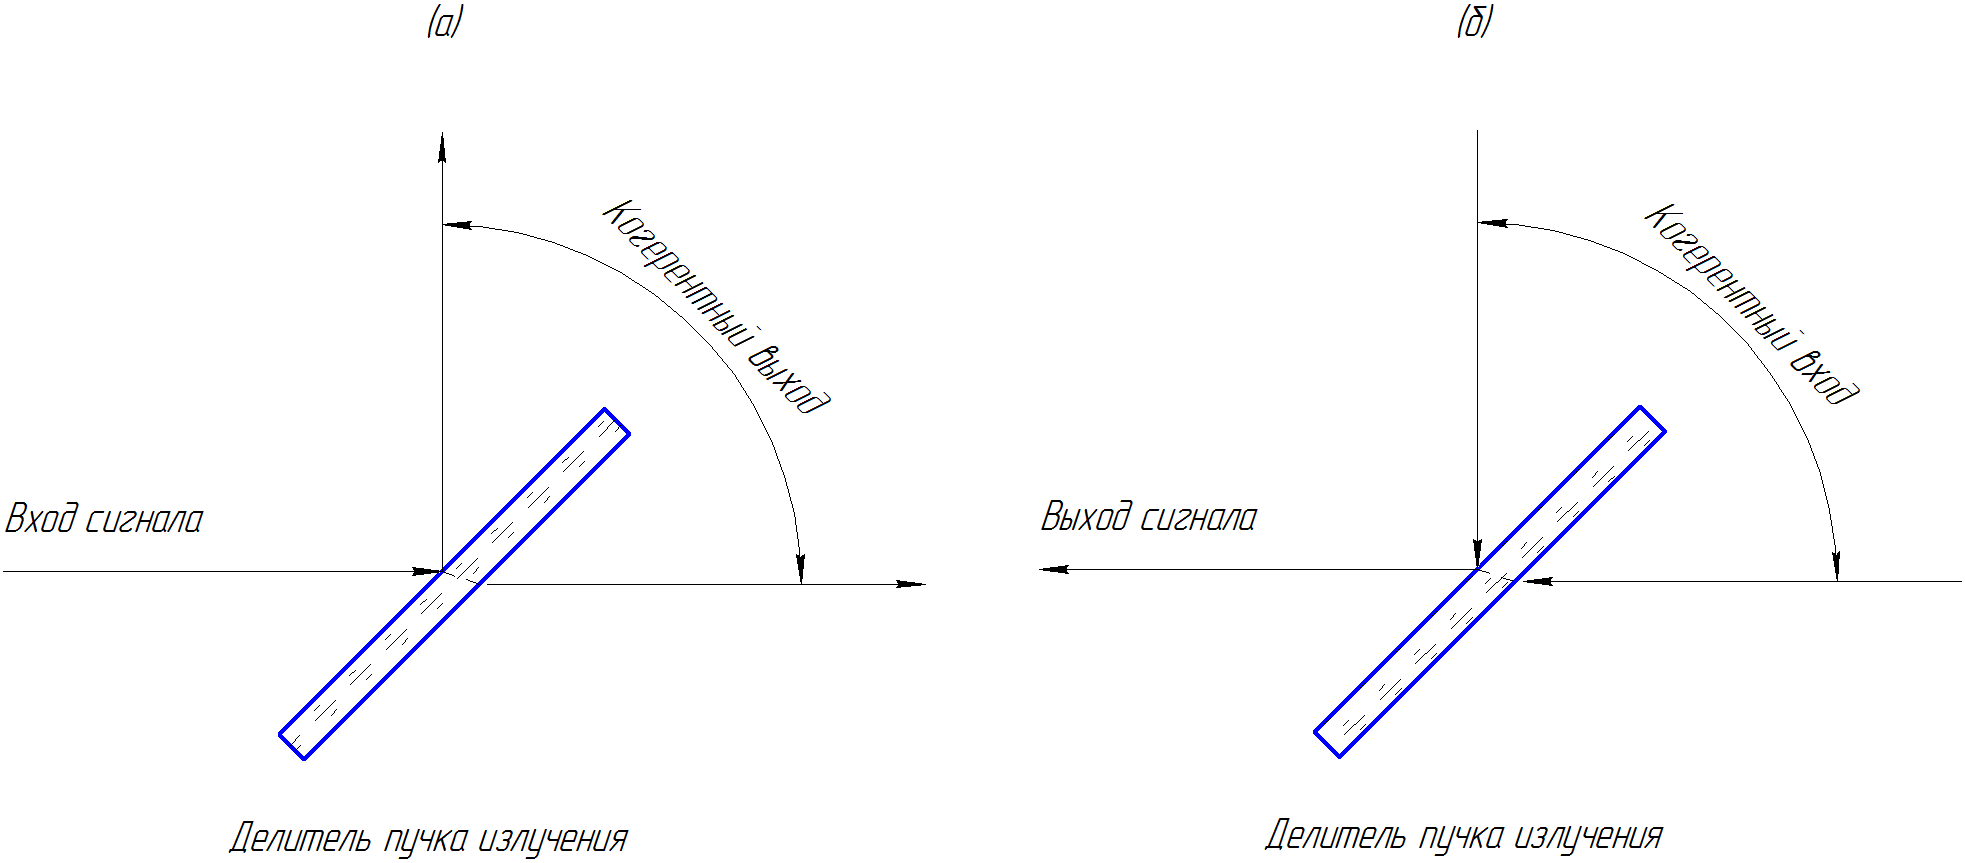
\includegraphics [scale=0.2] {jain_4_14}
  \caption{Делитель пучка излучения 50:50 (а) является когерентным объединителем излучения при использовании его в обратном нарпавлении (б).}
  \label{img:jain_4_14}
\end{figure}

Можно лучше понять суть пассивного механизма блокировки, если рассматривать продольные моды резонатора. Интервалы между продольными модами резонатора с эффективной длиной $L_{eff}$ определяются как $\Delta\nu=c/2 \cdot n \cdot L_{eff}$. Суперпозиция продольных мод отдельных лазеров приводит к формированию общих мод резонатора, или супермод всякий раз, когда моды совпадают для каждого из них. Эти супермоды наиболее устойчивы, поскольку конструктивно смешиваются в объединяющем элементе и несут наименьшие потери. В упрощенном случае двух лазеров с различными длинами разделение смежных супермод $\Delta\nu_Y=c/2 \cdot n \cdot \Delta L$ и разделение между смежными продольными модами в пределах супермоды $\Delta\nu=c/2 \cdot n \cdot L_{avg}$, где $\Delta L$ и $L_{avg}$ различие в длине и средняя длина лазерного массива соответственно (рис.~\ref{img:jain_4_15}). Любой резонатор с высоким усилением и низким Q-фактором удовлетворит условию многократного резонанса и возбудит все эти супермоды. Это дает ему возможность самокорректироваться при случайных изменениях в длинах пути~\cite{Jain136}.

\begin{figure} [ht]
  \center
  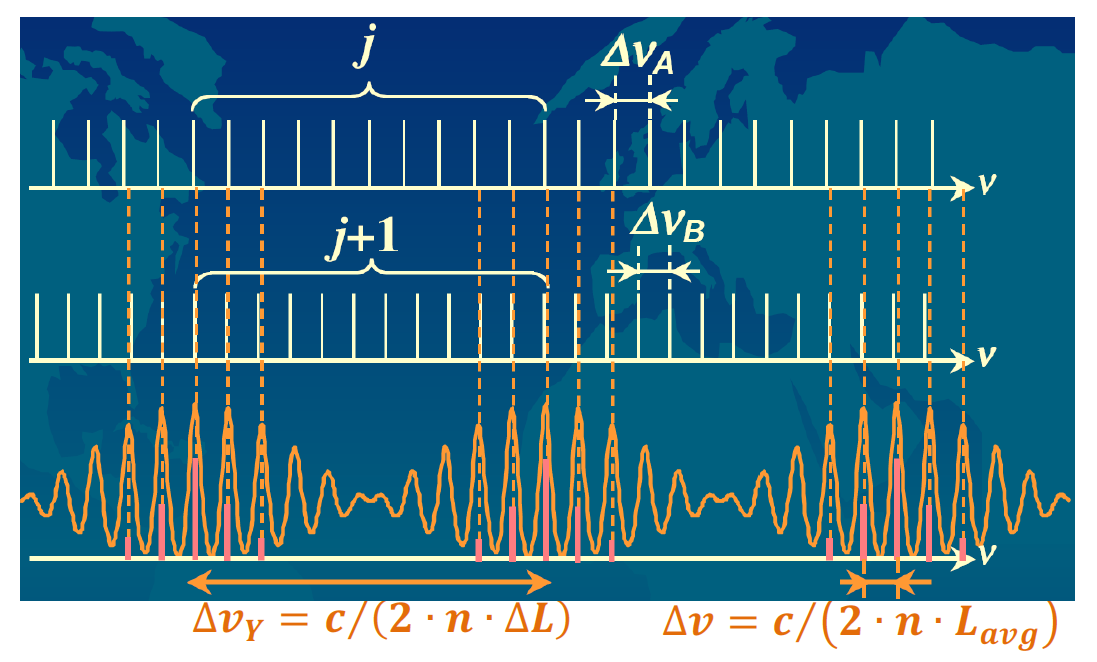
\includegraphics [scale=0.4] {jain_4_15}
  \caption{Формирование супермоды общего резонатора из-за перекрытия продольных мод отдельных лазеров~\cite{Jain136}.}
  \label{img:jain_4_15}
\end{figure}

Нужно отметить, что, хотя теория супермоды является хорошим инструментом для понимания механизма блокировки, она справедлива только при анализе <<холодного>> резонатора (нет усиления и поглощения) и не объясняет физические механизмы когерентной самоорганизации лазерных массивов. Практически, продольные моды отдельных лазерных резонаторов постоянно изменяются из-за возмущений в среде усиления, вызванных тепловыми эффектами (изменение в показателе преломления, длине материала и т.д.), изменением усиления, нелинейными эффектами и механическими возмущениями.

Используя этот метод несколько групп исследователей продемонстрировали когерентную блокировку волоконных лазеров. В силу устойчивости доминировало цельноволоконное исполнение с помощью 2x2 разветвителей волокна с древовидной архитектурой~\cite{Jain137,Jain138,Jain139,Jain140,Jain141,Jain142}. Лишь несколько работ было сделано в исполнении в свободном пространстве~\cite{Jain143,Jain144,Jain145}. В них объединено до 16 волоконных лазеров мощностью в несколько ватт. В компании Vytran утверждают, что достигли уровней объединенной мощности более чем 100 Вт от комбинации из 4 волоконных лазеров в цельноволоконной конфигурации. Однако, детали этого экспериментов включая анализ его устойчивости и эффективности объединения не были опубликованы~\cite{Jain146}. Сообщалось, что эффективность объединения очень чувствительна к величине обратной связи от каналов потерь, которую трудно подавить при цельноволоконной реализации~\cite{Jain147}.

Механизмы фазовой блокировки и масштабируемость размера массива в данном методе --- важная тема исследований. За последние годы были выполнены несколько теоретических и экспериментальных исследований~\cite{Jain134, Jain141, Jain148,Jain149,Jain150,Jain151,Jain152}. Хотя текущее состояние физического понимания является в лучшем случае базовым, определенные характеристики в плане эффективности объединения, требований к пропускной способности и стабильности мощности уже понятны. Большая часть последних работ указывает на снижение эффективности объединения с увеличением размера массива. Для системы из более чем 5 лазеров она падает ниже 90 \% (см. рис.~\ref{img:jain_4_16}a~\cite{Jain141}). Кроме того, экспериментальные и теоретические данные указывают на увеличение колебаний мощности (неустойчивость) как фактор $N^3$ с увеличением размера массива $N$ (см. рис.~\ref{img:jain_4_16}b)~\cite{Jain141}.

Причины этих явлений все еще являются объектом различных предположений. Однако, это ясно указывает на уменьшение когерентности больших лазерных массивов. Одно из возможных объяснений снижения эффективности объединения основано на теории супермод --- вероятность обнаружения случайного перекрытия в продольных модах отдельных лазеров уменьшается с увеличением числа лазеров. Как следствие, доступность многих продольных мод (и, следовательно, широкая пропускная способность) улучшает эффективность объединения и необходима для масштабирования больших массивов~\cite{Jain138}. Вопреки этой теории Минден и др.~\cite{Jain132} продемонстрировали пассивную блокировку двух одиночастотных волоконных источников и показали возможность когерентной блокировки источников с очень узкой шириной спектральной линии.

\begin{figure} [ht]
  \center
  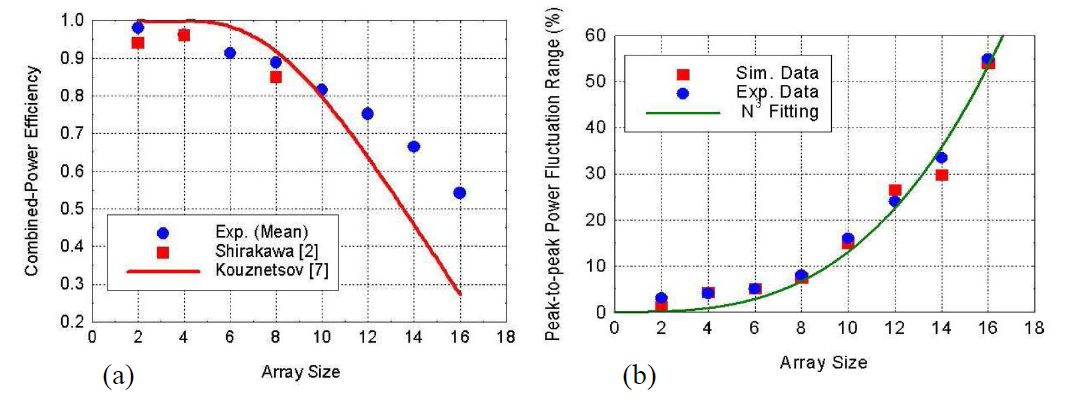
\includegraphics [scale=0.5] {jain_4_16}
  \caption{Масштабируемость размера массива для пассивного КОИ с  ветвителем 2x2: (a) эффективность объединения, (b) колебания мощности~\cite{Jain141}.}
  \label{img:jain_4_16}
\end{figure}

Другое возможное объяснение снижения эффективности объединения и увеличения колебаний объединенной мощности, является недостаточное взаимодействия между не соседними лазерными каналами. Вышеупомянутые исследования используют древовидную архитектуру с несколькими делителями 50:50. При такой реализации только самые близкие (соседние) волокна непосредственно взаимодействуют с друг другом. Таким образом, такая установка отбирает локальную супермоду для пары лазеров и может быть неспособна к эффективному отбору глобальной супермоды для всего массива. Производство волоконных делителей 1xN для объединения больших массив является очень сложной, но перспективной задачей. \textit{Для эффективного и масштабируемого пассивного объединения излучения важно, чтобы все лазерные каналы одновременно смешивались в одной точке, чтобы сгенерировать взаимно когерентную обратную связь для общего резонатора}.

Главный недостаток цельноволоконной архитектуры --- объединенный выход извлекается из одиночного волокна и, следовательно, не помогает в масштабировании мощности вне оптической прочности одиночного волокна. Установлено, что эффективность объединения уменьшается с увеличением накачки двух лазерных систем из-за нелинейности в волокне~\cite{Jain147}. Использование LMA волокон до некоторой степени может уменьшить этот эффект. Однако, использование больших волокон ухудшает качество пучка излучения, при этом полная объединенная мощность будет все еще ограничена непосредственно волокном. Таким образом, предпочтительно, чтобы \textit{объединенная мощность была в свободном пространстве}.

Очевидно, что реализация в свободном пространстве с возможностью обеспечения одновременного взаимодействия всех лазерных каналов является критической для интерференционного пассивного метода КОИ. Одной из многообещающих идей является использование объединителей ДОЭ Nx1 для пассивного КОИ~\cite{Jain37, Jain135, Jain153, Jain154}. Однако, известно лишь несколько его демонстраций с очень низкими мощностями и небольшими массивами. Леже и др. использовали бинарную фазовую решетку для блокировки шести полупроводниковых лазеров GaAlAs с эффективностью 68 \%~\cite{Jain154}. Используя сплошную поверхностную решетку Морел и др.~\cite{Jain135} пассивно объединили 3 легированным Nd одномодовых оптоволоконных лазера с эффективностью объединения 70 \%.

% \subsection{Резонатор Тальбо}

Этот метод основан на эффекте Тальбо для когерентных полей с бесконечной одномерной периодичностью. Такое поле точно воспроизводит само себя при распространении на расстояние Тальбо $Z_T=2\Lambda^2/\lambda$, где $\Lambda$ --- периодичность и $\lambda$ --- длина волны в свободном пространстве. Для массива из $n$ связанных лазеров могут быть определены $n$ супермод, характеризуемых различными фазовыми шагами $\Delta\phi=\phi_i-\phi_{i-1}$ между соседними эмиттерами. У каждой из этих супермод есть свое собственное характерное расстояние Тальбо, на котором она повторяет сама себя. Таким образом, помещая зеркало на расстояние $Z_M=Z_T/2$ соответствующая супермода может быть выборочно отражена и установлена обратная связь в резонаторе (см. рис.~\ref{img:jain_4_17})~\cite{Jain155}. Этот механизм обратной связи и высокие потери для всех других супермод позволяет осуществить фазовую блокировку всех эмиттеров в массиве. Этот метод подходит для фазовой блокировки одномерных массивов полупроводниковых диодных лазеров~\cite{Jain156}.

В случае волоконных лазеров данный метод особенно подходит для случая многосердцевинных волоконных структур~\cite{Jain155, Jain157,Jain158,Jain159,Jain160}. Многосердцевинное волокно состоит из несколько легированных сердцевин, обычно расположенных по кольцу внутри одной большой сердцевины накачки. Хотя явление самовоспроизведения все еще существуют в массиве связанных эмиттеров, предыдущее определение расстояния Тальба для бесконечного 1D массива больше не применимо к конечному 2D кольцевому массиву. Необходим более строгий расчет для оценки коэффициентов эффективного модового отражения $\gamma$ как функции расстояния до зеркала $Z_M$~\cite{Jain157}.

\begin{figure} [ht]
  \center
  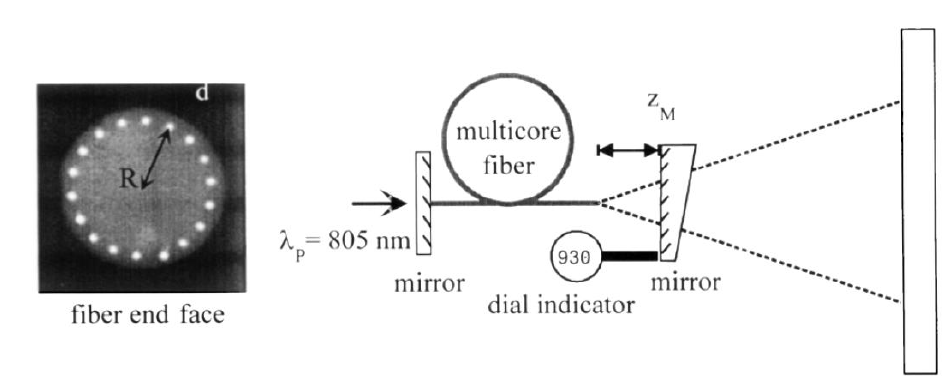
\includegraphics [scale=0.4] {jain_4_17}
  \caption{Схема многосердцевинного волоконного лазера с резонатором Тальбо~\cite{Jain155}.}
  \label{img:jain_4_17}
\end{figure}

В~\cite{Jain155} Враге (Wrage) и др. выполнили фазовую блокировку 18 легированных Nd эмиттеров, расположенных в кольцевом массиве, используя резонатор Тальбо в свободном пространстве. Авторы идентифицировали сосуществование разностных супермод и отклонений при изготовлении многосердцевинного волокна как вероятные причины низкой интенсивности на оси, когда интервал до зеркала соответствовал синфазной моде. В~\cite{Jain160, Jain161} пассивные волокна были приварены к обоим концам многосердцевинного волокна с 19 сердцевинами с формированием цельноволоконного устойчивого резонатора Тальбо и продемонстрировали выборочное возбуждение синфазной супермоды (рис.~\ref{img:jain_4_18}). В~\cite{Jain158} авторы использовали составные зеркала, чтобы одновременно увеличить дискриминацию между различными супермодами и сформировать выходной пучок излучения с высокой интенсивностью на оси.

Основные проблемы для масштабирования мощности лазеров в данном методе состоят в качестве производства многосердцевинных волокон, подавлении несовпадающих по фазе мод и увеличении числа элементов.

\begin{figure} [ht]
  \center
  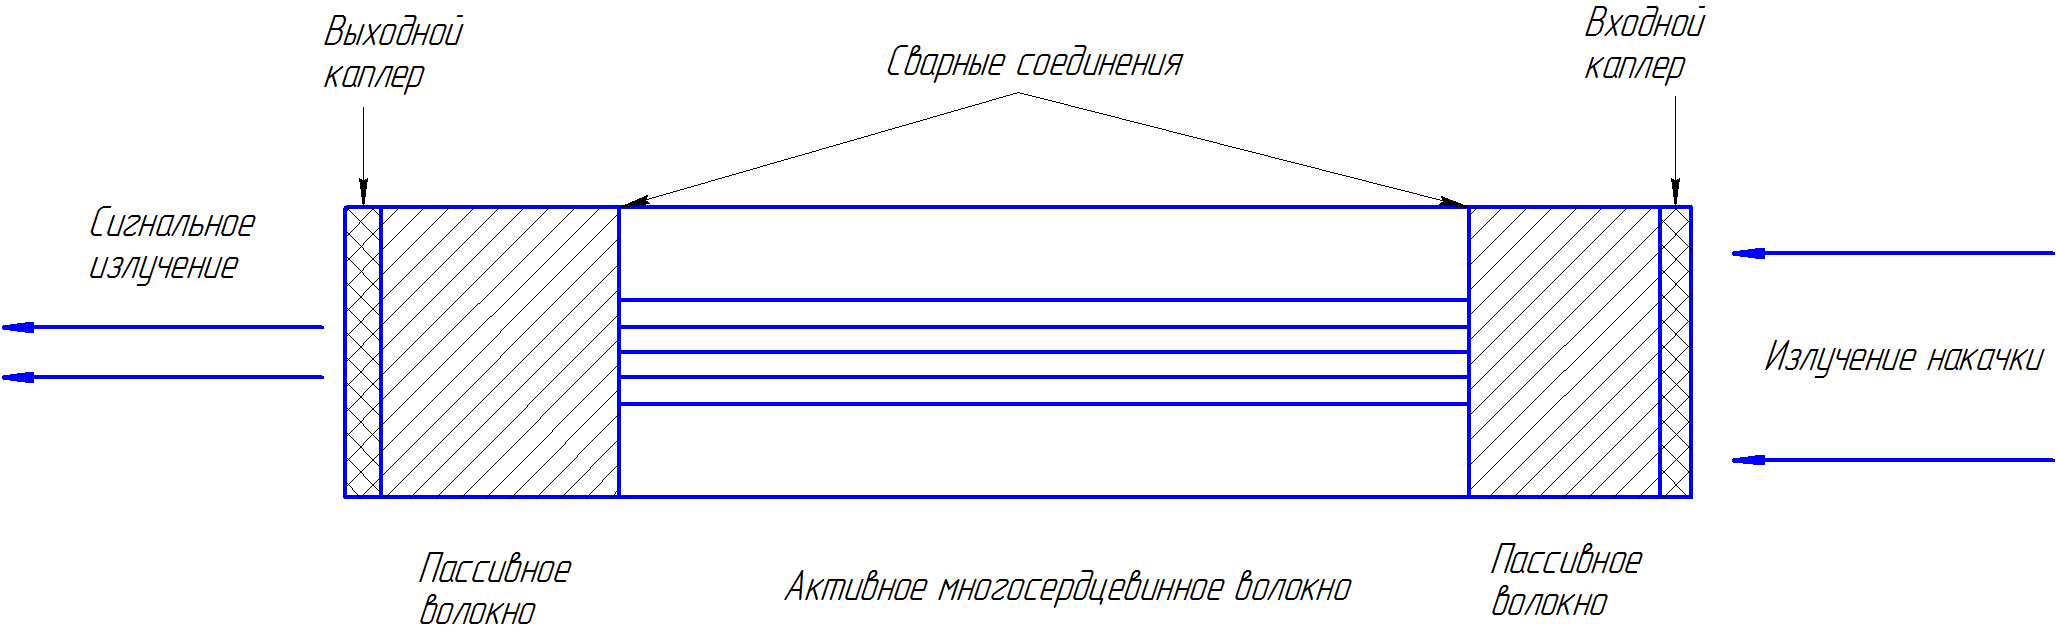
\includegraphics [scale=0.2] {jain_4_18}
  \caption{Пассивный КОИ с использованием цельноволоконного резонатора Тальбо.}
  \label{img:jain_4_18}
\end{figure}

% \subsection{Собственный фурье-резонатор}

Когерентное объединение лазеров, используя собственный фурье-резонатор (СФ-резонатор), основано на свойствах собственных функций Фурье. СФ-функция обладает фурье-преобразованием, при котором она является точной копией самой себя (рис.~\ref{img:jain_4_19}). Известно, что функция Гаусса и функция <<гребенки>> (пилообразная функция) обладают собственным фурье-преобразованием, и, при определенных условиях, может быть точными копиями самих себя~\cite{Jain162}. Например, гауссиана $A(x)=\exp(-x^2/a^2)$ с шириной $a$ является СФ-функцией, если $a=1/\sqrt{\pi}$. Точно так же функция <<гребенки>> $B(x)=\sum\delta(x-n\cdot b)$ c интервалом $b$  является СФ-функцией, когда $b=1$. В~\cite{Jain163} Коркорэн показал, что при надлежащем выборе параметров функция, полученная сверткой гауссианы с произведением гауссовой функции и функции <<гребенки>> также является СФ-функцией:
\begin{equation}\label{eq4.4-1}
  F(x)=A(x)\otimes [B(x)\cdot C(x)]=\sum_n \exp[-(x-nb)^2/a^2]\exp[-(nb/c)^2],
\end{equation}
где $A(x)$ и $C(x)$ --- гауссовы функции с шириной $a$ и $c$ $(a<c)$ соответственно и $B(x)$ является функцией <<гребенки>> с интервалом $b$. На рис.~\ref{img:jain_4_20} показан пример этой функции.
\begin{figure} [ht]
  \center
  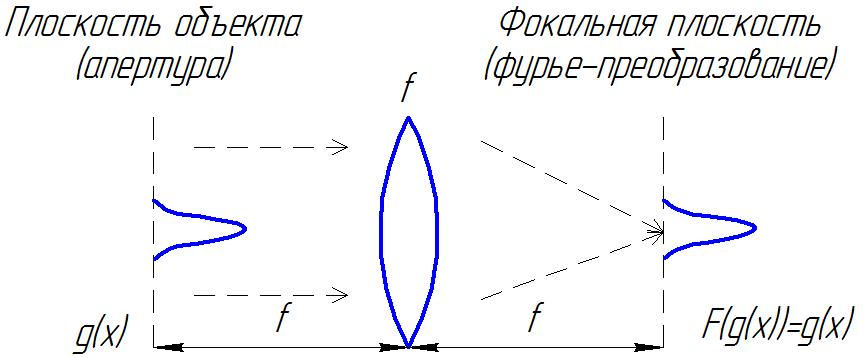
\includegraphics [scale=0.3] {jain_4_19}
  \caption{Определение собственных фурье-функций.}
  \label{img:jain_4_19}
\end{figure}
\begin{figure} [ht]
  \center
  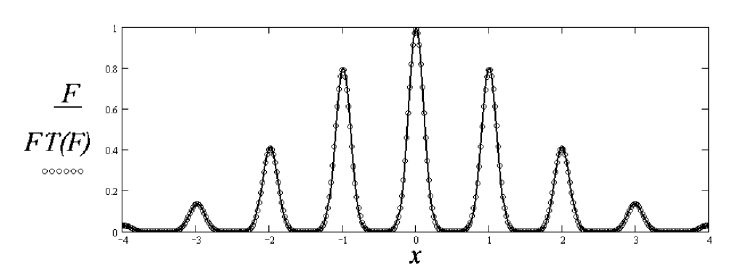
\includegraphics [scale=0.4] {jain_4_20}
  \caption{Пример собственной фурье-функции из уравнения \eqref{eq4.4-1}.}
  \label{img:jain_4_20}
\end{figure}
Схема на рис.~\ref{img:jain_4_19} может быть свернута сама на себя с формированием СФ-резонатора, если обрезать линзу на половину и поместить ее в контакт с зеркалом (рис.~\ref{img:jain_4_21}). Отметим, что, так как теперь перемещение пучка через линзу происходит дважды, то, чтобы иметь то же самое эффективное фокусное расстояние $F_L$, реальное фокусное расстояние линзы должно быть $2\times F_L$. Теперь ПФ поля во входной плоскости, которая находится на расстоянии $L=F_L$ от поверхности зеркала, накладывается на себя после прохода туда и обратно в СФ-резонаторе.
\begin{figure} [ht]
  \center
  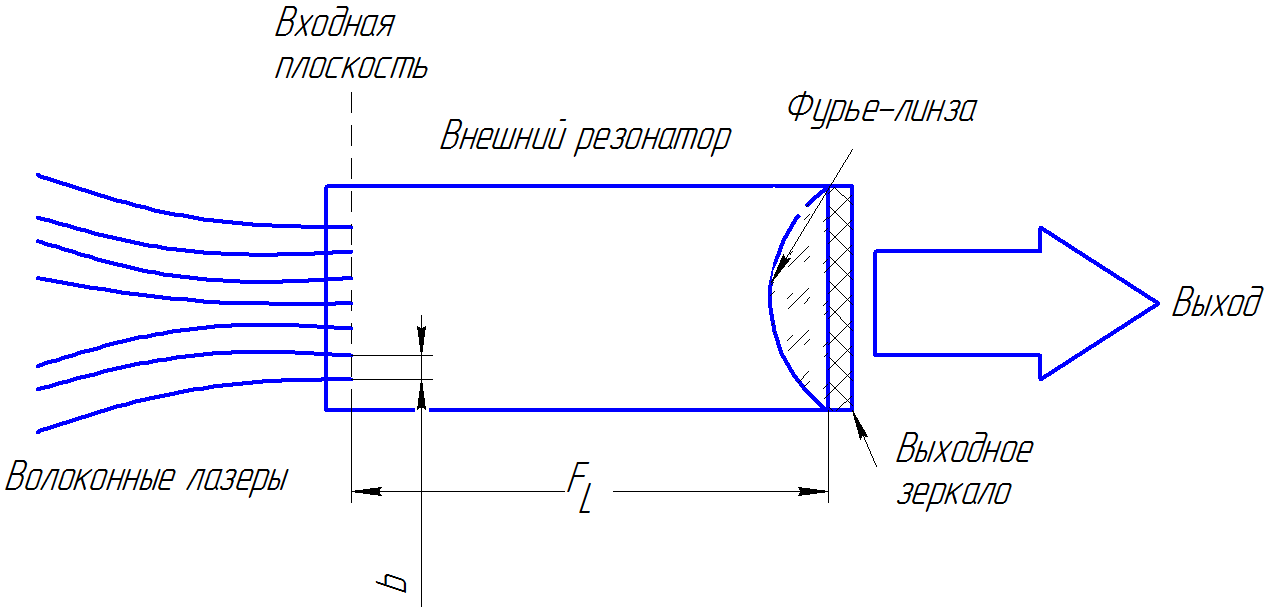
\includegraphics [scale=0.3] {jain_4_21}
  \caption{Свернутый СФ-резонатор.}
  \label{img:jain_4_21}
\end{figure}
Было показано, что СФ-функция уравнения~\eqref{eq4.4-1} имеет одну степень свободы, и выбирая ширину гауссианы как свободный параметр, другие два параметра должны удовлетворять соотношениям:
\begin{equation}\label{eq4.4-2}
  b=\sqrt{F_L\cdot\lambda}\sqrt{1-\pi^2\frac{a^4}{(F_L\cdot\lambda)^2}}\approx\sqrt{F_L\cdot\lambda},
\end{equation}
\begin{equation}\label{eq4.4-3}
  c=\sqrt{F_L\cdot\lambda}\times\frac{b}{\pi\cdot a}\approx\frac{F_L\cdot\lambda}{\pi\cdot a}.
\end{equation}
В СФ-резонаторе на рис.~\ref{img:jain_4_21} когерентное объединение излучения может быть достигнуто, если располагать массив волокон с шириной выходного пучка излучения отдельных эмиттеров равной $a$ и расположенных на равных интервалах с периодичностью $b$ во входной плоскости. Выходы волоконных лазеров аппроксимируются гауссовым профилем излучения и при использовании массива микролинз могут иметь требуемую ширину. Параметр $c$ определяет огибающую обратной связи и следовательно число элементов в массиве. На практике принимаются компромиссные решения по сравнению с идеальной СФ-системой (бесконечное количество элементов, предельная эффективность) путем усечения массива до конечного числа элементов. Показано, что потери могут составить менее 2 \% от циркулирующей мощности, если выбирать число элементов как~\cite{Jain164}
\begin{equation}\label{eq4.4-4}
  N\approx0,8\times\frac{b}{a}.
\end{equation}
При таком расположении N элементов во входной плоскости интерференционная картинка обратной связи, сформированная после прохода излучения туда и обратно (которая является по существу той же самой, как и выход массива) эффективно устанавливает обратную связь в отдельных волокнах. Как следствие фурье-природы резонатора обратная связь с каждым элементом включает вклады от всех элементов, что вынуждает производить коллективную лазерную генерацию. Некогерентная часть выхода отдельных эмиттеров не способна к подобным преобразованиям в СФ-резонаторе и несет высокие потери, не способствуя обратной связи вообще. Таким образом, СФ-резонатор является чрезвычайно эффективным селектором мод для одномодового резонатора. В~\cite{Jain164,Jain165,Jain166} дано всестороннее описание СФ-резонатора и выполнен анализ пассивного фазирования.

В~\cite{Jain167} Коркорэн экспериментально продемонстрировал устойчивый массив 7 сфазированых волоконных лазеров в СФ-резонаторе с объединенной выходной мощностью 0,4 Вт. В планах масштабирование до массива из 21 волоконного лазера с высокой выходной мощностью~\cite{Jain168}. Также была изучена пассивная комбинация с СФ-резонатором для многосердцевинных волоконных лазеров с затухающей связью~\cite{Jain166}.

Ограничение СФ-резонатора связано с качеством выходного пучка излучения. В дальней зоне излучение массива из N элементов имеет N пиков (рис.~\ref{img:jain_4_20}). Необходимы подходящие методы заполнения апертуры, чтобы собрать мощность в <<хвостах>> одиночных дифракционно-ограниченных пучков излучения, что добавляет сложности этой системы. Другая проблема в масштабировании к большему размеру массива содержится непосредственно в уравнении~\eqref{eq4.4-4}. Чтобы увеличить число элементов в массиве, размер эмиттеров должен быть уменьшен или интервал между ними увеличен --- оба этих фактора приводят к низкому коэффициенту заполнения. Этот метод, как все другие пассивные методы КОИ, также восприимчивы к различиям в относительной длине оптического пути элементов массива. Идеальное СФ-отображение возможно только при синфазных входных пучках излучения. Любая относительная разность фаз изменяет распределение в дальней зоне и ухудшает эффективность связывания.

% \subsection{Пространственная фильтрация в плоскости Фурье}

У данного пассивного метода КОИ есть некоторые общие черты с СФ-резонатором в том, что пространственная фильтрация происходит в фокальной плоскости фурье-линзы, но не ограничена СФ-функциями. Чтобы сколлимировать выход массива из N оптических усилителей используется массив микролинз, расположенных в архитектуре со стыкованными апертурами в плоскости S2 как показано на рис.~\ref{img:jain_4_22}~\cite{Jain169}.
\begin{figure} [ht]
  \center
  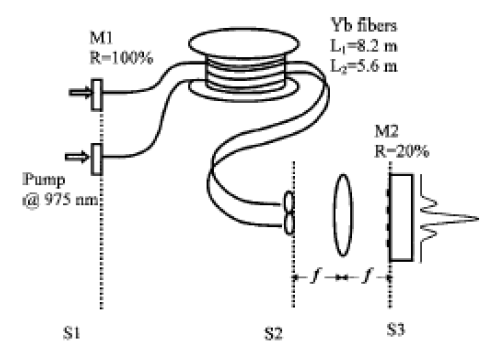
\includegraphics [scale=0.45] {jain_4_22}
  \caption{Схема пространственной фильтрации в плоскости Фурье~\cite{Jain169}.}
  \label{img:jain_4_22}
\end{figure}
Для проекции картинки в дальней зоне этого коллимированного массива в плоскости S3 используется фокусирующая линза. Когда все выходы массива будут когерентными и синфазными, у результирующей картинки поля в плоскости S3 будет виден пик  интерференции. Чтобы передать только центральный пик в эту плоскость нужно поместить пространственный фильтр и сгенерировать высокие потери для несовпадающих по фазе мод и достижения фазовой блокировки. При использовании кольцевого резонатора этот метод масштабировался до высоких мощностей и больших массивов~\cite{Jain170,Jain171,Jain172}. Архитектура кольцевого резонатора с пространственной фильтрацией показана на рис.~\ref{img:jain_4_23}. Одномодовое волокно выступает в качестве пространственного фильтра, и обратная связь массива усилителей обеспечивается использованием 1xN волоконного делителя, который завершает кольцевой резонатор.
\begin{figure} [ht]
  \center
  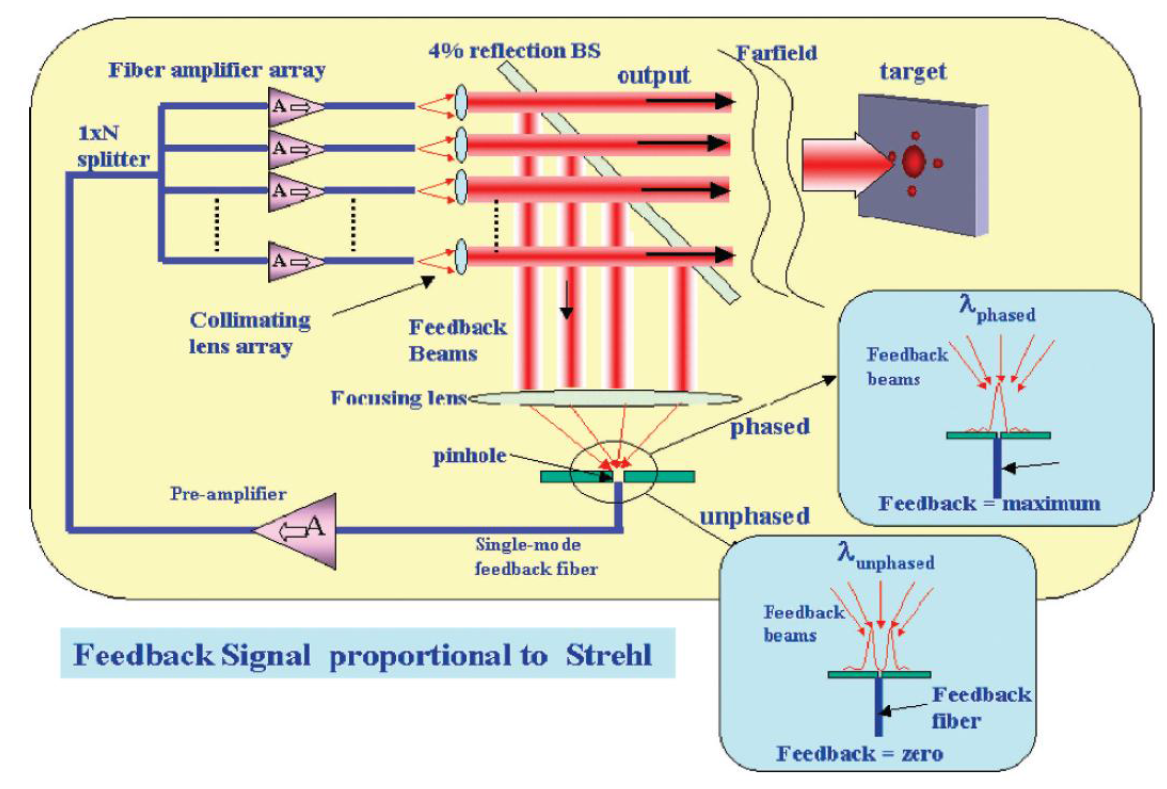
\includegraphics [scale=0.4] {jain_4_23}
  \caption{Кольцевой резонатор с пространственной фильтрацией для пассивного КОИ~\cite{Jain170}.}
  \label{img:jain_4_23}
\end{figure}
Фурье-линза формирует в дальней зоне картинку массива усилителей в его фокальной плоскости, где SMF выровнен относительно оптической оси. В случае синфазности всех мод и, соответственно, максимальной интенсивности на оси эффективность ввода в SMF является самой высокой по сравнению со всеми другими модами, что в свою очередь приводить к максимальной обратной связи в массиве. Таким образом, объединенный кольцевой резонатор пассивно выбирает моду с максимальной интенсивностью на оси в дальней зоне. Разработан детальный анализ выбора супермоды в таком кольцевом резонаторе~\cite{Jain173, Jain174}.

Этот метод был впервые исследован в Northrop Grumman, которым также принадлежит патент на него~\cite{Jain175}. Продемонстрирована пассивная блокировка 8 волокон в линейном массиве и 4 волокон в 2D массиве при низких и умеренно высоких объединенных мощностях. На рис.~\ref{img:jain_4_24} показаны ключевые результаты, полученные в~\cite{Jain171}, где каждый отдельный лазер имеет мощность 200 Вт с объединенной мощностью 710 Вт. Однако, лазеры работали c большой спектральной шириной в 30 нм.

\begin{figure} [ht]
  \center
  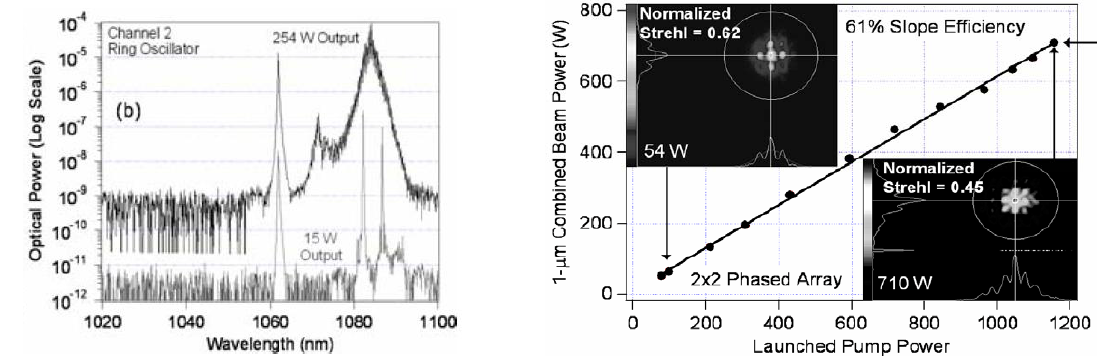
\includegraphics [scale=0.4] {jain_4_24}
  \caption{Результаты~\cite{Jain171}: спектральная ширина каждого лазера (слева); мощность объединенной системы (справа).}
  \label{img:jain_4_24}
\end{figure}

Хотя последние результаты достаточно многообещающие, есть ряд оставшихся без ответа вопросов и свойственных недостатков. Как в любом методе со стыкованной апертурой в дальней зоне на <<хвостах>> теряется существенная доля мощности. Даже в этом случае наблюдаемое в дальней зоне соотношение Штреля в~\cite{Jain171} намного хуже, чем теоретический предел для массива с тем же самым коэффициентом заполнения. Авторы приписывают это недостаткам конструкции и тепловым проблемам без дальнейшего анализа. Ухудшение качества излучения может также иметь место, если массив не является взаимно когерентным и не синфазным. Никакие тесты для того, чтобы определить степень когерентности не выполнялись. Широкая спектральная полоса (короткая длина когерентности) и постоянно колеблющийся спектр отдельных лазеров, вероятно, приводит к нестабильности картинки в дальней зоне на SMF. Это может привести к колебаниям объединенной мощности, эффективности и качества излучения. Ни о каких измерениях устойчивости объединенного пучка излучения не сообщается.

Что еще более важно, есть свойственная проблема выбора только синфазных мод. В дальней зоне у картинки с некогерентного массива также есть пик на оси. Таким образом, некогерентное излучением от массива всегда устанавливает обратную связь с резонатором и полное подавление невозможно. При высоких мощностях накачки обратная связь, полученная от некогерентных и несовпадающими по фазе мод, может быть достаточной, чтобы пройти порог и начать генерацию. Другая проблема --- связь внеосевых усилителей в одномодовое оптоволокно (с конечным NA) может быть менее эффективной, чем связь усилителей вблизи оси при больших массивах. Минимизация потерь в резонаторе не гарантирует, что будет выбрана только синфазная мода. Анализ Леже и др. показывает, что чувствительность к длины оптического пути при такой архитектуре пространственной фильтрации намного ниже. Вне определенной ошибки длины пути потери для всех мод равны и результирующая картинка в дальней зоне --- некогерентная суперпозиция всех мод~\cite{Jain176}.

%\subsection{Фазирование с помощью ВРМБ. Обращение волнового фронта}

Наиболее популярным подходом при разработке сфазированных волоконных
массивов является электрооптическое контролирование фазы в каждом
волоконном канале MOPA-установки. Хотя различные научные группы
используют несколько разные подходы при фазировании, суть
заключается в том, чтобы разделить излучение задающего генератора
(ЗГ) на несколько каналов, усилить излучение в каждом из них,
измерить относительную фазу в каждом канале и создать отклик на
фазовые модуляторы для того, чтобы зафиксировать фазу выходного
излучения с каждого канала. Этот подход был успешно применен при
фазировании каналов массивных усилителей \cite{121,122,123}. Однако
существуют определенные трудности, связанные с большим количеством
оптических элементов в установке и сложностью управляющей
электроники. При увеличении количества усиливаемых каналов
соответственно растет и сложность установки. По этой причине
необходимо разработать точный метод фазирования без необходимости в
сложной управляющей электронике.


Один из пассивных методов фазирования использует явление
вынужденного рассеяния Мандельштама --- Бриллюэна (ВРМБ) в процессе,
известном как обращение волнового фронта (ОВФ). На рис. 1 показана
схема эксперимента по двухканальному фазированию с помощью которой
проиллюстрируем данный процесс. В данной конфигурации излучение ЗГ
разделяется на два канала. Проходя по своему собственному
оптическому пути, излучение в каждом канале усиливается и
фокусируется на одну и ту же ОВФ-среду. Разница в длине оптических
путей приводит к ненулевой разности фаз двух пучков, падающих на
ОВФ-среду. Так как оба пучка фокусируются на ОВФ-среду (в данном
случае - оптическое волокно), то при наложении мы получаем одиночный
пучок с модулированной фазой и интенсивностью в соответствии с
разностью фаз. Фазы двух пучков складываются, и стоксов пучок
восстанавливает оптический путь в каждом канале, что приводить к
нулевой разности фаз между пучками. Именно этот процесс называют
обращением волнового фронта \cite{124,125}. Хотя конечной целью
данного процесса является фазирование усиленных пучков, в 80-х годах
прошлого века было выполнено большое количество работ по
исследованию явления ОВФ без использования усиления в каналах.
Большинство работ обсуждены в обзорной статье Мойера \cite{125},
ниже приведены лишь наиболее важные результаты.


Н. Г. Басов и его группа \cite{126} были первыми, кто успешно
продемонстрировал коррекцию разности фаз путем разделения лазерного
пучка на два канала и их объединения на ОВФ-решетке. Кроме
демонстрации концепции, авторы также установили необходимость в
фокусировании пучка на одной и той же области среды. Если излучение
лазеров собрать в одной области среды, создаваемое акустическое поле
становится общим для всех пучков и становится возможным
соответствующее фазирование. С другой стороны, если каждый пучок
возбуждает свою собственную акустическую волну, случайная природа
генерации ВРМБ из-за тепловых шумов приводит к случайной
относительной фазе пучков. Эту идею Басова подтверждает его
демонстрация когерентного объединения перекрывающихся пучков и
некогерентного объединения в случае, когда пучки не перекрываются.


Группа Н. Г. Басова исследовала также эффективность фазирования
пучков. После фазирования остаточная разность фаз ($\delta$ в долях
периода волны), происходящая из малой разности частот излучения
накачки и стоксовых пучков, дается соотношением

\begin{equation}\label{delta}
   \delta = \Delta_B \Delta_L,
\end{equation}

где $\Delta_B$ - это ВРМБ-сдвиг волнового числа и $\Delta_L$ -
разность длин оптических путей. Ограничение, налагаемое данным
соотношением, заключается в том, что для желаемой точности фазировки
необходимо точно контролировать измеряемую разность длин оптических
путей (РОП) между каналами \cite{124,127}. Например, лазерное
излучение с длиной волны 1064 нм в кварцевом волокне претерпевает
ВРМБ-сдвиг ~16ГГц ($\Delta_B = 53,3  m^{-1}$). При требуемой
максимальной ошибке фазирования 0,1 волны максимальная допустимая
разность оптических путей составляет 1,9 мм. Достичь данный уровень
точности оптических путей для массива волоконных усилителей крайне
сложно. К счастью, как было проверено в той же работе, относительная
ошибка фазирования циклична относительно РОП совокупности волн, что
приводит к повторению хороших степеней фазирования (т.е., $\delta
\approx 0, 1, 2,$ и т.д.). Последним требованием для получения
хорошей степени фазирования является малость (к единице) отношения
полной разности оптических путей к длине когерентности лазера.


Группа Ричарда Мойера исследовала коррекцию ошибки фазирования с
целью получения когерентно объединенной совокупности лазерных
пучков. В их эксперименте излучение импульсного одночастотного
лазера с длиной волны 355 нм разделялось на два канала. Оба пучка
проходили свой пассивный оптический путь и фокусировались на одной
ОВФ-среде. В эксперименте также использовался интерферометр
поперечного сдвига (ИПС, рис.2) для исследования свойств фазирования
пучков и определения успешной фазовой подстройки. В работе ИПС
использовался как диагностическая установка, устройство которой
представлено ниже.


Интерферометр поперечного сдвига, показанный на рис.2, состоит из
пары непокрытых клиновидных линз, внутренние поверхности которых
параллельны друг другу. Параллельные пучки, проникающие в систему,
частично отражаются от обоих поверхностей. В результате одного из
отражений пучок сдвигается относительно другого отраженного пучка,
так что создаются три зоны интерференции (см. рис. 2). Две внешние
области интерференции являются областями самоинтерференции каждого
из пучков с ним же, но отраженным от другой поверхности (со
смещенным). Центральная область есть интерференция пучков обоих
каналов. Фазирование достигается, когда полосы на всех трех областях
совпадают (полосы непрерывны по всем трем областям).


Кроме вышеизложенного в рамках исследований ОВФ-фазирования пучков
рядом научных групп были изучены эффекты обратного рассеяния
\cite{125,128}, характеристики пучков (ширина спектра, отношения
мощностей, изменения поляризации) \cite{129}, а также выполнено
теоретическое исследование эффективности фазирования
\cite{1210,1211}. Также были проведены эксперименты по
масштабированию мощности, используя фазирование двух импульсных
лазерных пучков, каждый из которых в своем канале содержит усилитель
Nd:YAG \cite{1212,1213}. Вероятно, наибольшую трудность в ранних
экспериментах представляло точное выравнивание ОВФ-решетки
\cite{129,1211,1214}. Именно поэтому в текущих исследованиях, как
правило, в качестве ОВФ-среды используется многомодовое волокно
\cite{1215}. При соответствующей геометрии волновода можно уйти от
требования перекрывания пучков (см. выше), что значительно упростит
реализацию ОВФ-фазирования. Данный подход был реализован в работе
\cite{1216}. В экспериментах в качестве ЗГ использовался
одночастотный кольцевой лазер (NPRO - non-planar ring oscillator) с
длиной волны 1064 нм, шириной спектра < 5 кГц и мощностью 700 мВт,
выполненный компанией Lightwave Electronics. Схема установки
представлена на рис. 2. Ее описание можно найти в работе
\cite{1216}. Из рис. 2 видно, что излучение после прохождения
усилителей (усиления), накладывается друг на друга с помощью
поляризационного фильтра. После этого, суммарный пучок вводится в
волокно как ОВФ-среду, где происходит их когерентное объединение для
генерации обращенной волны. В качестве ОВФ-среды использовалось
многомодовое волкно (Corning) с ядром 50 мкм/0,2 NA.

\begin{figure}
\centering
%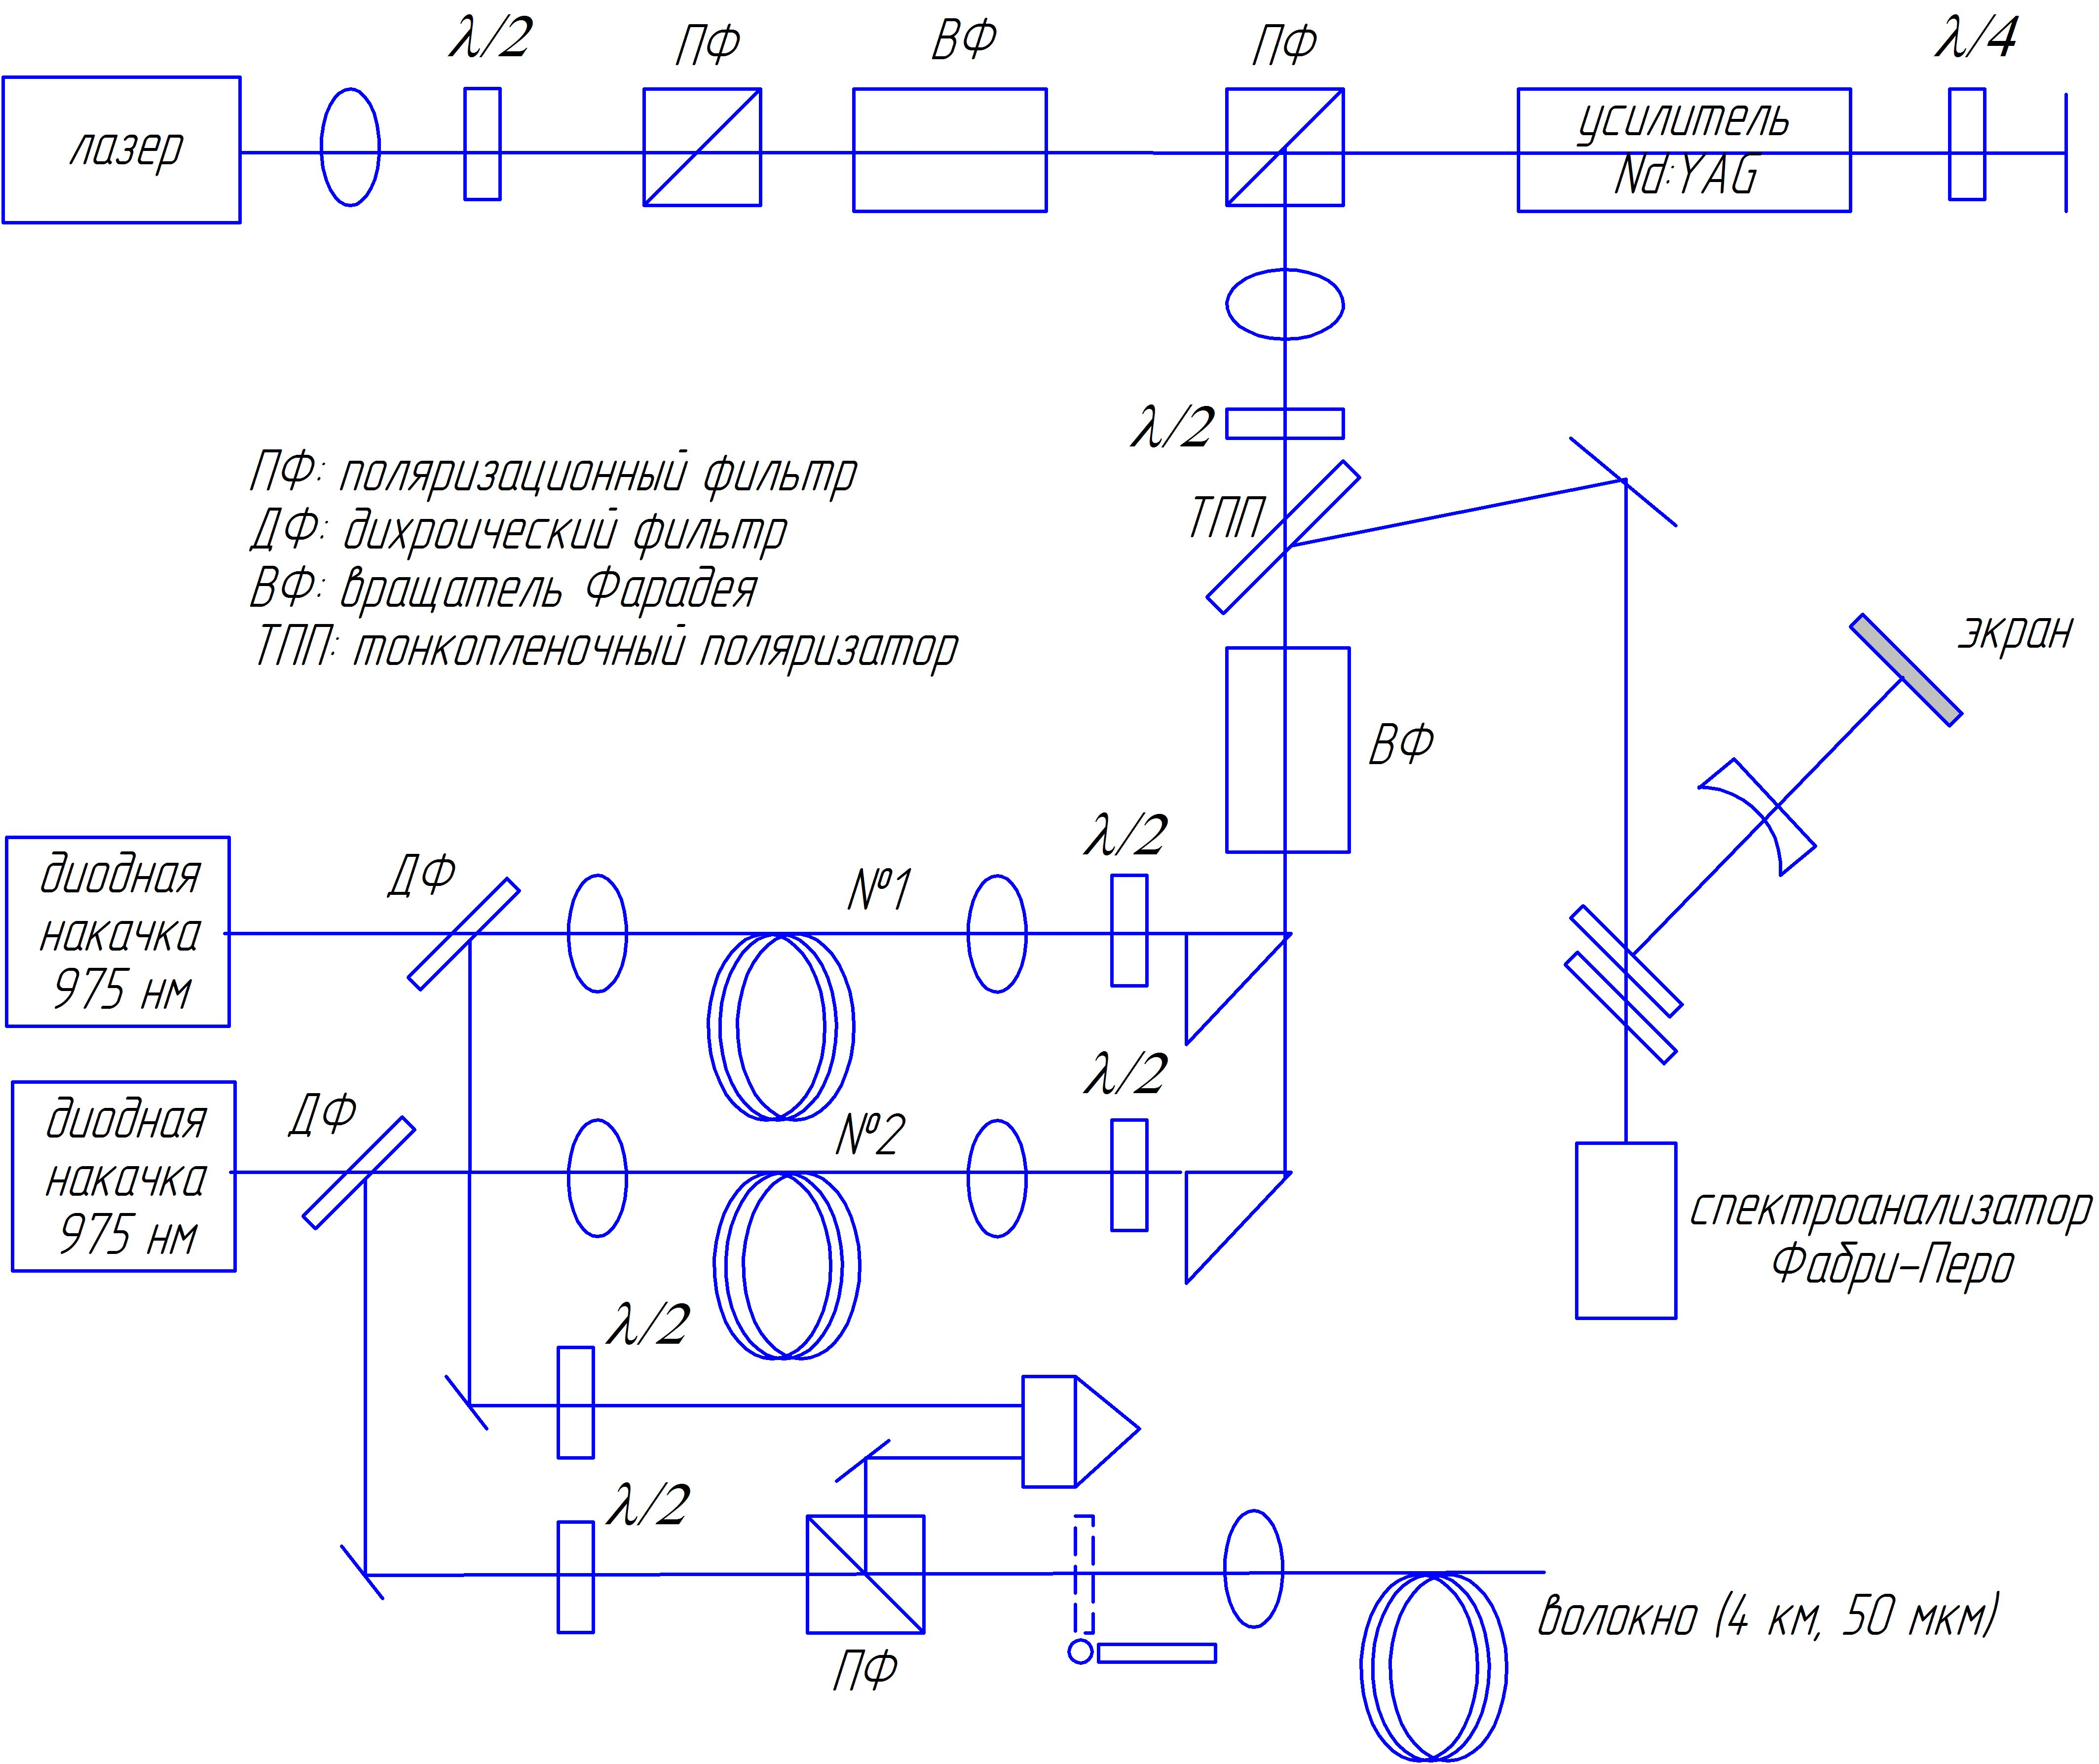
\includegraphics[width=5in,height=4.20in]{sbs.bmp}\\
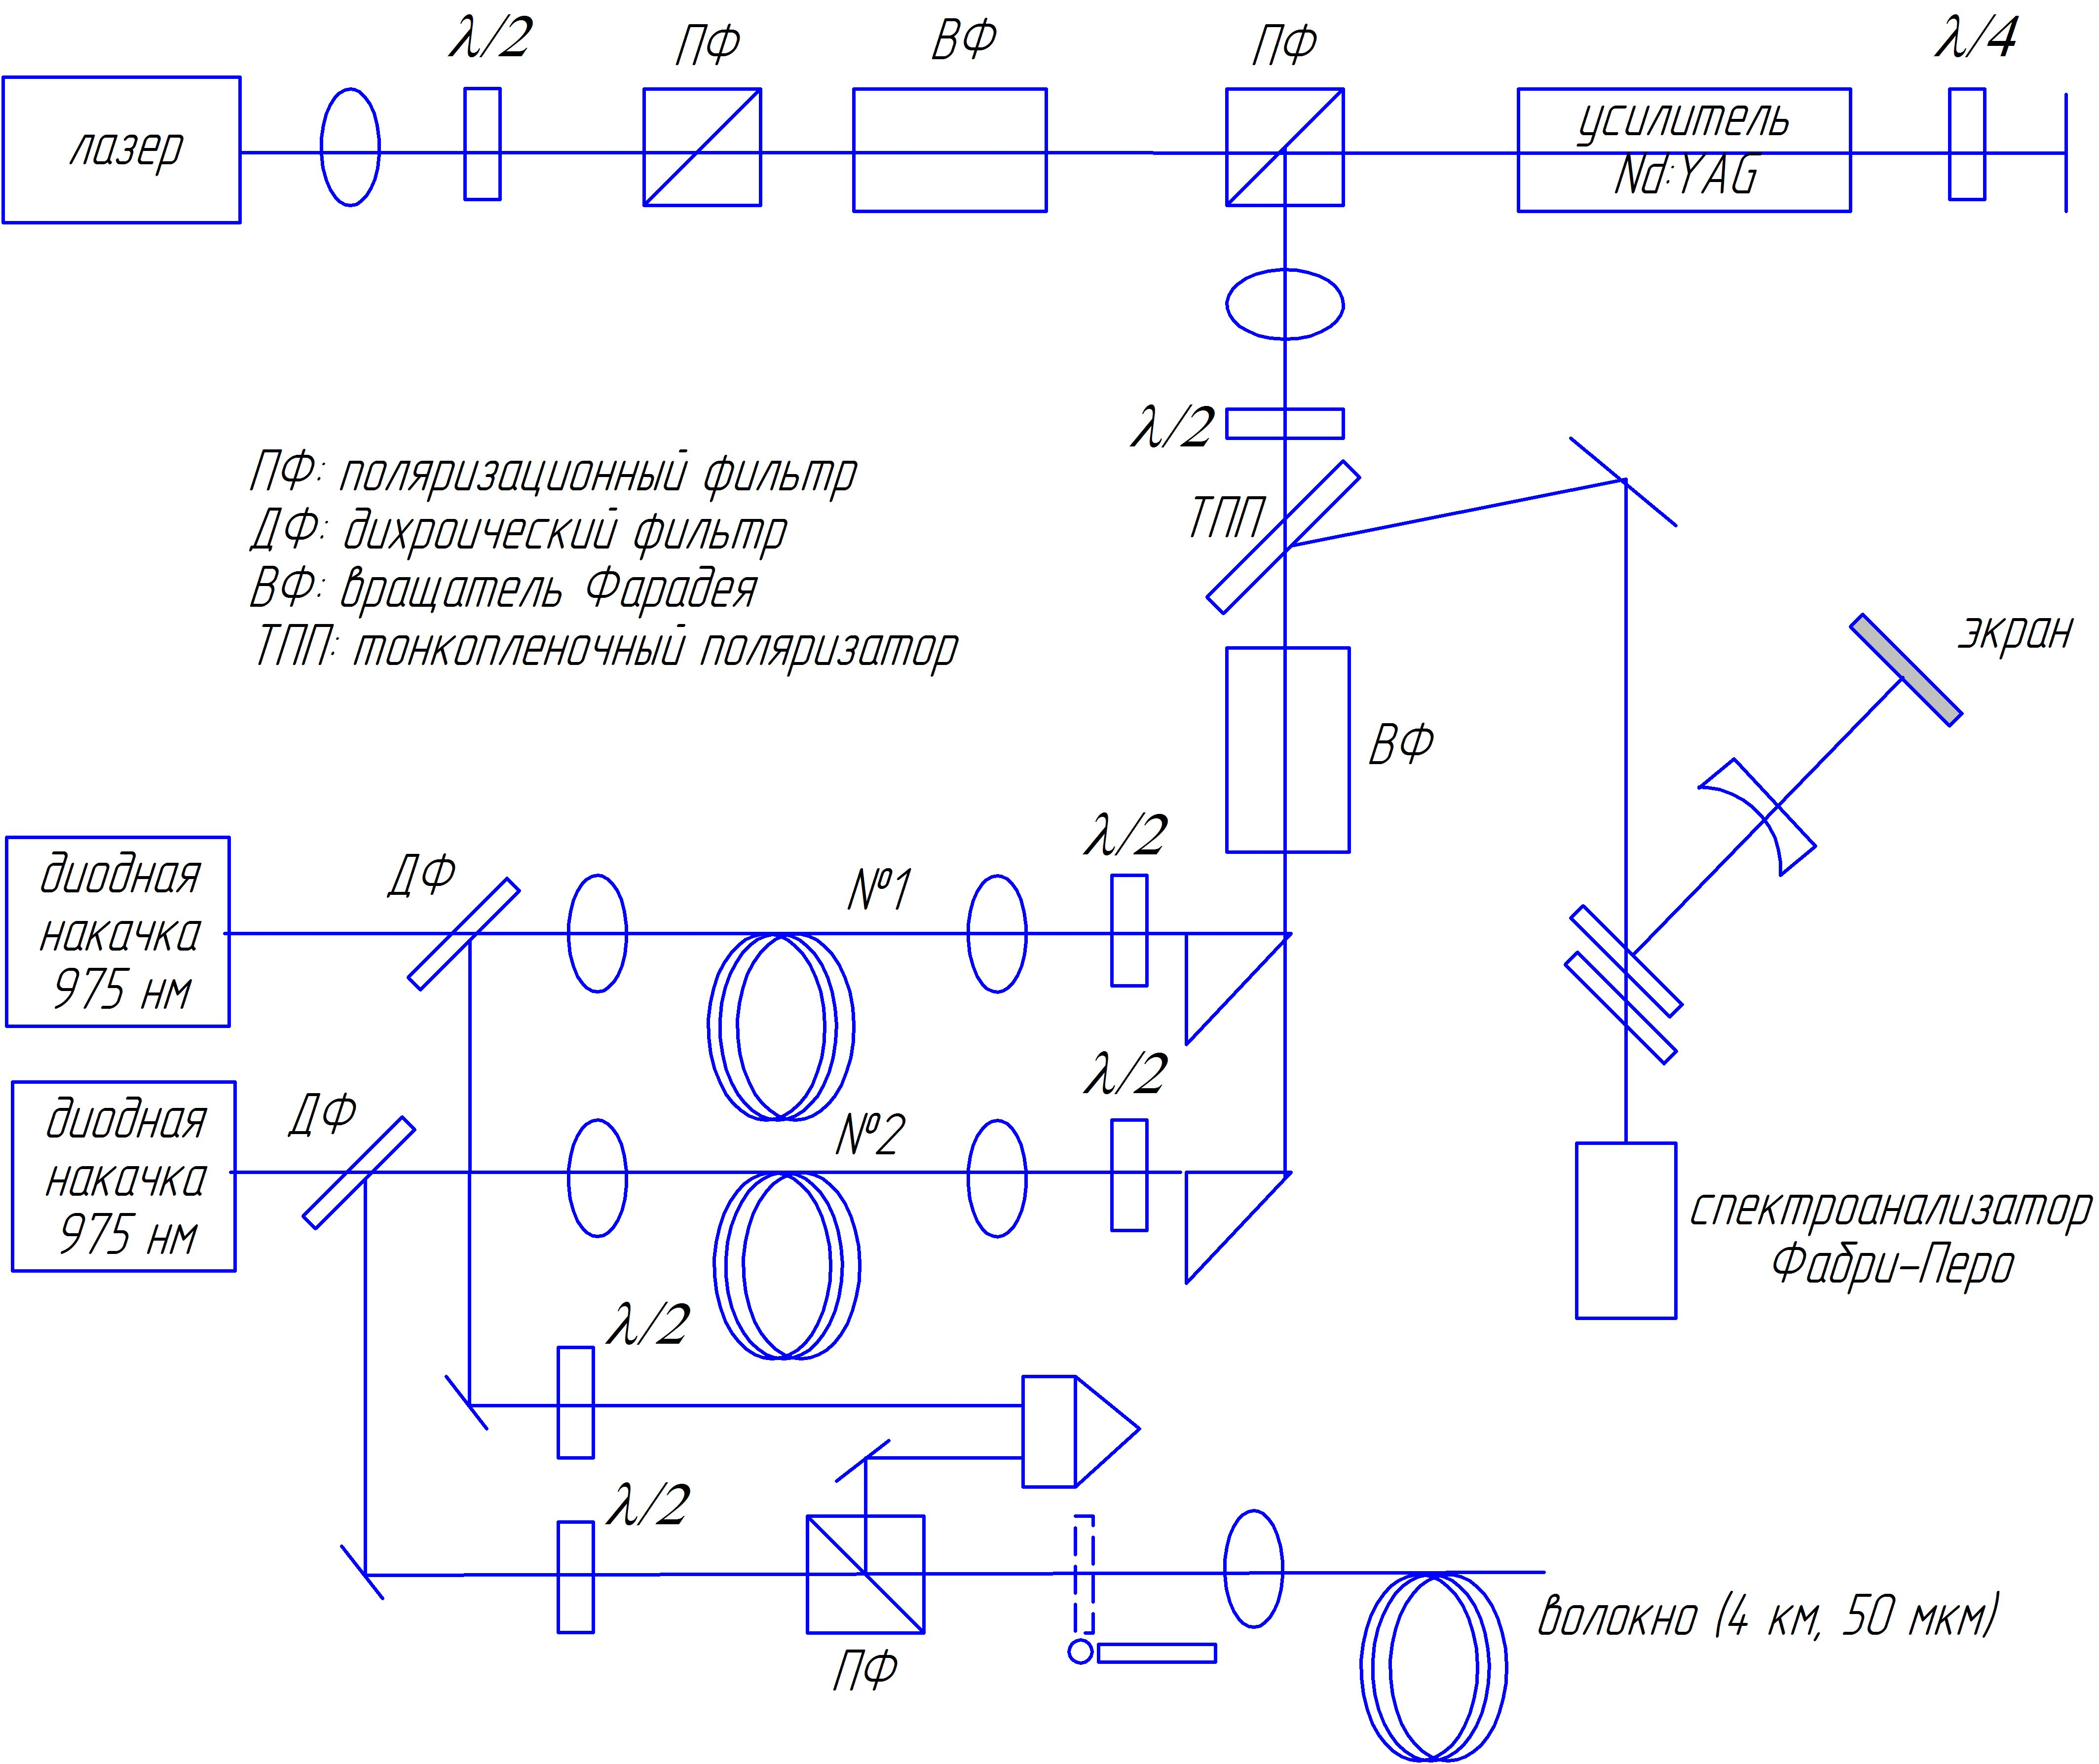
\includegraphics[width=5in,height=4.20in]{sbs.jpg}\\
\caption{Экспериментальная схема ОВФ-фазирования.} \label{sbsbeam}
\end{figure}

Смещение, полученное в результате ВРМБ, для волокна диаметром 50 мкм
(LMA-волокно) составляет 15,2 $\pm$ 0,2 ГГц ($\Delta_B = 50,7
m^{-1}$). Используя вышеприведенную формулу было оценено изменение
оптического пути по периоду волны, которое составило $\Delta_L =
19,7 \pm 0,3$ мм. При проведении эксперимента, мощность излучения на
входе усилителей составляло 440 мВт и 480 мВт для 1-го и 2-го
каналов соответственно. Эффективность перекачки в ядро составляла
порядка 60~\%. Суммарная мощность на выходе равна 5,3 Вт. Таким
образом, исходя из значения входной мощности 920 мВт, эффективность
усиления экспериментальной установки составила 475~\%. Эффективность
преобразования накачки в усилителе составила $\approx 40$~\%. В итоге, в
данной работе была достигнута выходная мощность 5 Вт при
использовании пассивного метода фазирования. Было впервые
продемонстрировано фазирование пучков непрерывных усилителей с
помощью волоконного ОВФ-зеркала.

%\subsection{Спектральное обращение волнового фронта}

Рассмотрим электромагнитную волну, распространяющуюся в направлении
оси $z$,
\begin{equation}\label{eq13.1}
    E_1(r,z,t) = E_1(t,r) exp(i(\omega t - kz)) \equiv E_1
    exp(i(\omega t - kz + \phi(t,r)))
\end{equation}
где, $\omega, k, E_1$ и $\phi(t,r)$ --- радиальная частота, момент,
амплитуда и фаза (медленно меняющаяся во времени и в пространстве)
оптического поля, $r$ есть поперечная координата. Временное
изменение фазы дает частотную полосу, тогда как пространственное
изменение дает отклонение волнового фронта излучения от плоского.
Сопряженное по фазе поле дается выражением
\begin{equation}\label{eq13.2}
    E_c(r,z,t) = E_1^{\ast}(t,r) exp(i(\omega t \pm kz)) \equiv E_1
    exp(i(\omega t \pm kz - \phi(t,r)))
\end{equation}
В уравнении~\eqref{eq13.2} знак <<$\pm$>> означает, что сопряженное по
фазе поле может распространятся относительно исходного поля как в
прямом, так и в обратном направлении. Одним из замечательных свойств
сопряженного по фазе поля является то, что в случае, когда в
уравнении~\eqref{eq13.1} возникает $\phi(t,r)$ как результат
искажения поля при распространении в среде, распространяющееся в
противоположном направлении сопряженное по фазе поле может привести
к компенсации $\phi(t,r)$ и таким образом восстановить
первоначальное качество поля. Именно эта особенность широко
исследуется в пространственной области~\cite{1313}.

Согласно уравнениям \eqref{eq13.1} и \eqref{eq13.2}, спектральное
фазовое сопряжение (СФС) --- это процесс, который генерирует
выходной пучок, частотный спектр которого является комплексно
сопряженным спектру входного пучка. В ряде статей в качестве
средства для восстановления временной формы пучка~\cite{1314,1315},
обращения дисперсионного размывания и избавления от фазовой
самомодуляции ~\cite{1312,1316,1317,1318} было предложено
использовать четырехволновое смешение (ЧВС) как средство реализации
СФС.

Способность ЧВС к спектральному ОВФ напрямую следует из закона
сохранения энергии. Если направляющиеся навстречу друг другу (в $+z$
и $-z$ направлениях) волны с одинаковой частотой $\omega$
взаимодействуют в кубической нелинейной среде с опорной волной
частоты $\omega + \delta\omega$, распространяющейся в направлении
$+z$, частота результирующей волны будет
\begin{equation}\label{omega}
    \omega+\omega-(\omega+\delta\omega) = (\omega-\delta\omega)
\end{equation}
Схематическая диаграмма такого взаимодействия, показанная на рис.~\ref{f132},
демонстрирует, что спектр сигнальной волны есть
сопряжение спектра опорной волны относительно частоты волны накачки.


Несмотря на то, что ЧВС потенциально очень эффективный процесс,
опубликовано лишь небольшое количество экспериментальных работ по
исследованию его СФС свойств. Причина кроется в компенсация
дисперсии в импульсных волоконно-оптических каналах, которые, как
было показано, обладают довольно низкой эффективностью ($\approx 0,1
\%$)~\cite{1319,1320}. Причина в том, что, во-первых, широкий спектр
сигнала в таких системах требует использования короткого времени
затухания нелинейности, которая в свою очередь не должна быть
высокой~\cite{1321}, а во-вторых, длина нелинейного взаимодействия
не может быть велика из-за неизбежных фазовых расхождений при
невырожденном ЧВС~\cite{1322}.


Прорыв в данном вопросе был сделан в работе~\cite{1300}, где было
обнаружено, что ВРМБ является эффективным способом СФС и, т.о.,
обеспечивает восстановление временной когерентности в
обратно-рассеянном стоксовом сигнале~\cite{1310}. Так как данный
процесс не требует дополнительных волн накачки, как при ЧВС, то в~\cite{1300}
этот процесс был назван спектральным обращением
волнового фронта (СОВФ, \emph{spectral self-phase conjugation}).
Данное явление есть ничто иное как временной аналог хорошо
известного пространственного обращения волнового фронта при ВРМБ, и
как и последний, является следствием ВРМБ.

Чтобы понять СОВФ свойства ВРМБ, упомянем некоторые особенности
ВРМБ, предсказанные классической теорией, хорошо описанной в работах
Кролла~\cite{1323} и Танга~\cite{1324} в середине 60-х годов
прошлого века. ВРМБ представляет собой нелинейный оптический
процесс, в котором стоксово смещение рассеянного излучения
усиливается в оптически прозрачной среде путем параметрического
взаимодействия с накачкой и электрострикционно индуцированной
звуковой волной. Выходная стоксова эмиссия затем усиливается
спонтанной эмиссией и, поэтому, полностью стохастическое~\cite{1325}
сужение спектра усиления является единственным изменением выходного
спектра~\cite{1324,1325}. Однако, в настоящий момент следует
обратить внимание на экспериментальный факт того, что стоксовый
эмиссионный сигнал (как результат ВРМБ), возбуждаемый непрерывным
монохроматическим излучением накачки в оптическом волокне, не
является полностью стохастическим, содержа хорошо выраженную
\emph{постоянную} амплитуду~\cite{1326}. В действительности,
существует множество ранних экспериментальных подтверждений данного
факта, показывающих, что стоксова эмиссия далека от 100~\% модуляции
(несмотря на то, что в них использовали импульсное излучение накачки
в объемных~\cite{1327,1328} и волноводных~\cite{1329,1330} средах).
Подтверждения этого можно найти также и в более поздних работах по
ВРМБ, где в оптических волокнах использовалась непрерывная накачка~\cite{1332,1333,1334,1335}.
Все эти данные находятся в полном
противоречии с классическим пониманием ВРМБ, который предсказывает
полную стохастичность стоксового сигнала. Как было упомянуто выше,
непрерывная компонента фактически появляется только когда мощность
накачки выше пороговой мощности ВРМБ, т.е. когда $N\geq1,2$ (см.
рис.~\ref{f13.3} и~\ref{f13.4}).
\begin{figure}
\centering
%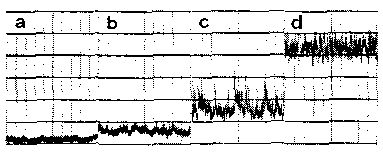
\includegraphics[width=2.55in,height=1.04in]{f133.bmp}\\
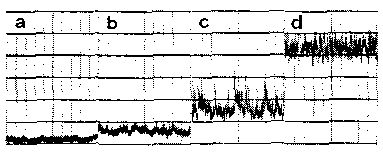
\includegraphics[width=2.55in,height=1.04in]{f133.jpg}\\
\caption{Временная запись стоксовой эмиссии в двумодовом волокне
длиной 650 м и диаметром сердцевины 9мкм при N=1,1(a), N=1,5(b),
N=2(с), N=9(d), масштаб времени 2 мкс~\cite{1300}.} \label{f13.3}
\end{figure}

\begin{figure}
\centering
%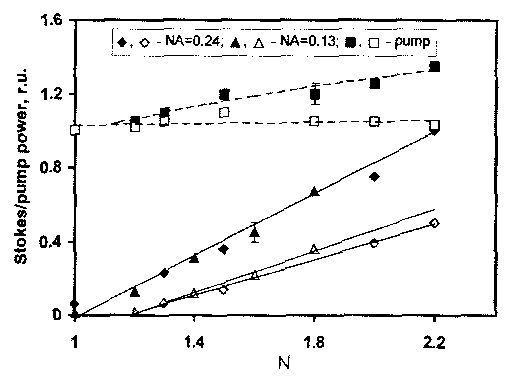
\includegraphics[width=3.41in,height=2.54in]{f134.bmp}\\
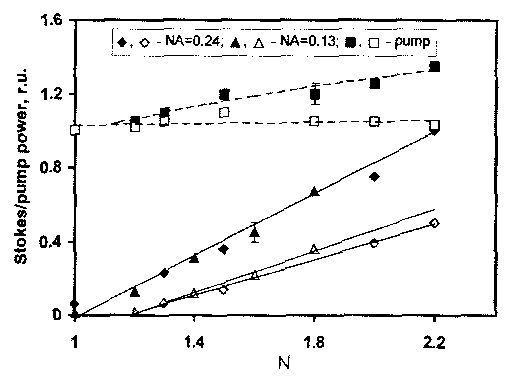
\includegraphics[width=3.41in,height=2.54in]{f134.jpg}\\
\caption{Пиковый+стабильный (закрашенные символы) и стабильные (не
закрашенные символы) амплитуды стоксова (сплошная линия) и
прошедшего (пунктирная линия) излучений по отношению к N для двух
одномодовых волокон с числовой апертурой NA=0,24 и L=200 м и NA=0,13
и L=100 м~\cite{1300}.} \label{f13.4}
\end{figure}
Вблизи порога ВРМБ ($N<1,2$) в стоксовом сигнале четко проявляется
динамика хаотических пиков (ДХП) со $\approx 100 \%$ глубиной
модуляции (см. рис.~\ref{f13.3}а), что находится в четком согласии с
классическим пониманием ВРМБ. Эти сведения говорят о том, что
появление постоянной компоненты является следствием изменения ВРМБ
взаимодействия при $N\geq1,2$. В дальнейшем в работе \cite{1300}
было показано, что при $N\geq1,2$, когда появляется постоянная
стоксова компонента (см. рис.~\ref{f13.4}), в проходящем через среду
излучении накачки появляется ДХП компонента, т.е., будучи изначально
монохроматическим, спектр проходящего излучение становится уширенным~\cite{1336}.
При $N<1,2$ такого рода уширение незначительно, и в
спектре нет постоянных стоксовых компонент (см. рис.~\ref{f13.3}а).

С первого взгляда эти результаты кажутся парадоксальными: постоянная
стоксова эмиссия появляется, когда в области взаимодействия
излучение накачки спектрально уширено, и стоксов сигнал полностью
стохастичен, когда излучение накачки монохроматично по всей длине
области взаимодействия (см. рис.~\ref{f13.5}). Распознавая таким
образом, что постоянная эмиссия по существу является восстановлением
спектральной когерентности падающего излучения накачки, мы приходим
к аналогии со знакомым восстановлением пространственной
когерентности путем классического ОВФ при ВРМБ~\cite{1337}. Таким
образом, часть области ВРМБ взаимодействия, где имеет место
спектральное уширение спектра накачки, можно рассматривать как
<<плоскость фазового искажения>> в спектральной области таким же
образом, как такая плоскость рассматривалась в пространственной
области. Излучение накачки с искаженным (многочастотным) спектром
(см. рис.~\ref{f13.5},II,а) попадает в область линейного ВРМБ, где
взаимодействует с многочастотной стоксовой эмиссией (см. рис.~\ref{f13.5},II,c),
 инициированной спонтанным рассеянием.


\begin{figure}
\centering
%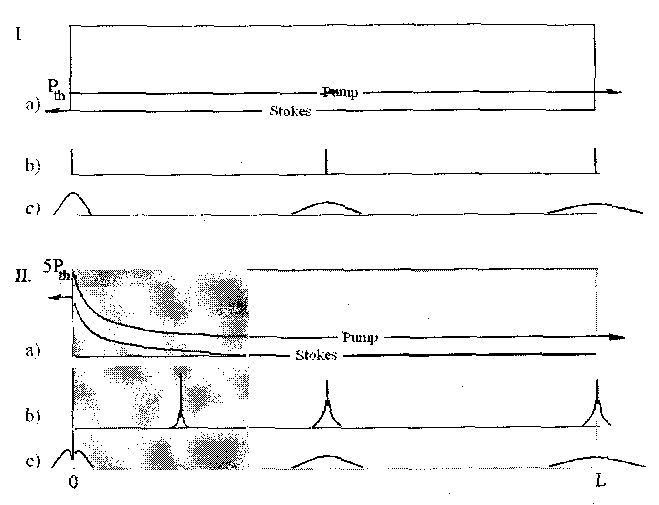
\includegraphics[width=4.39in,height=3.37in]{f135.bmp}\\
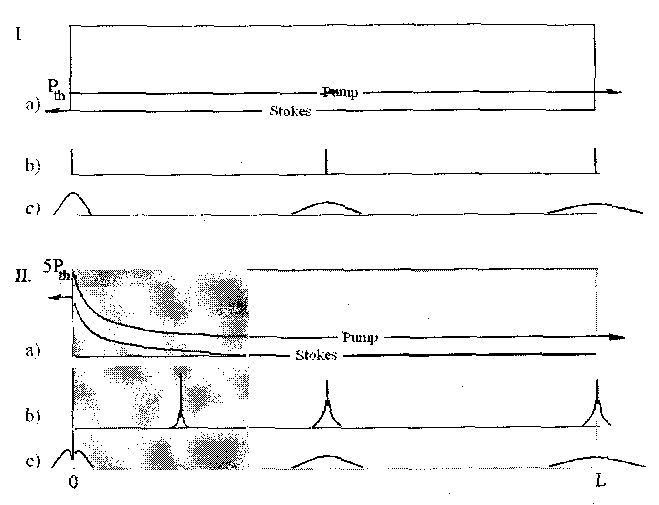
\includegraphics[width=4.39in,height=3.37in]{f135.jpg}\\
\caption{Схематическая диаграмма распределения мощности (a) накачки
и стоксова сигнала, спектра (b) накачки и (с) стоксова сигнала вдоль
области взаимодействия длиной L для мощности накачки (I) вблизи
порога ВРМБ и (II) $\sim$ пятикратного порога ВРМБ~\cite{1300}.}
\label{f13.5}
\end{figure}


Согласно современному пониманию ОВФ при ВРМБ, это состояние,
необходимое для привилегированного усиления обращенных компонент в
стоксовом излучении~\cite{1338}. Эта основная и хорошо установленная
модель пространственного ОВФ при ВРМБ~\cite{1338}, подразумевает
мультипоперечные моды и поэтому, находится за пределами
классического плосковолнового описания ВРМБ~\cite{1324}, но при этом
все еще остается одночастотной моделью.


\begin{figure}
\centering
%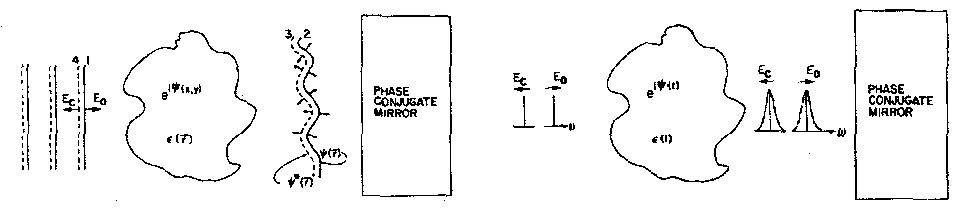
\includegraphics[width=5in,height=1.12in]{f136.bmp}\\
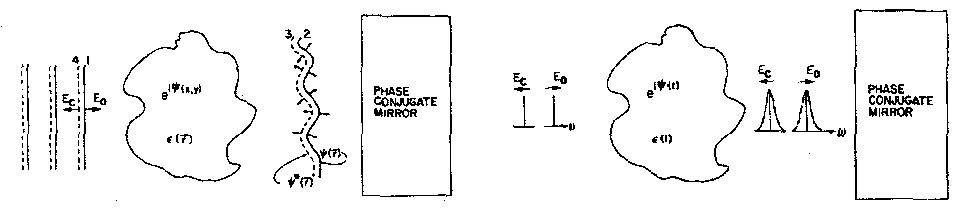
\includegraphics[width=5in,height=1.12in]{f136.jpg}\\
\caption{Двупроходная схема компенсации пространственных (слева)  и
спектральных (спарва) искажений с помощью ОВФ-зеркал~\cite{1300}.}
\label{f13.6}
\end{figure}

В теоретической работе Аникеева~\cite{1339}, к сожалению мало
цитируемой, рассматривающей ВРМБ взаимодействие мультипоперечных и
мультичастотных оптических полей в объемной среде, показывается, что
наряду с пространственным ОВФ, спектр стоксового сигнала должен быть
обращением спектра излучения накачки. Очевидно, что теоретическая
модель для объемной среды применима также и для ВРМБ в многомодовом
волокне. Не так очевидно, что теория может быть применима и для
одномодового волокна. Последнее связано с тем, что оптическая волна,
распространяющаяся в одномодовом волокне, не является плоской волной
и по этой причине в этом волокне вызывает спектральное уширение
стоксовой эмиссии~\cite{1326}. Так как ВРМБ обеспечивает обращение
спектра так же, как и обращение волнового фронта излучения накачки,
ФС излучение способно компенсировать как спектральное искажение, так
и пространственные искажения, вызванные распространением через
фазоискажающую среду (см. рис.~\ref{f13.6}). Необходимым условием
при этом является то, что процесс, ответственный за спектральное
уширение излучения накачки, удовлетворяет \emph{теореме о поправках
искажения}. Эта теорема, сформулированная для пространственной
области~\cite{1340}, утверждает, что: <<Если волна $E_1(r)$
распространяется слева направо через произвольную диэлектрическую
среду без потерь, и, если в некоторой области пространства
генерируется ее сопряженная по фазе реплика $E_c(r)$, то $E_c$ будет
распространяться справа налево через диэлектрическую среду оставаясь
везде фазовым сопряжением $E_1$>>. Доказательство этой теоремы
для пространственных искажений монохроматической волны основано на
подстановке уравнения распространения оптического поля в волновое
уравнение Гельмгольца. Для пространственно-временного случая не
монохроматической оптической волны $E_1(r,z,t)$ должно быть
подставлено в более общее уравнение вида
\begin{equation}\label{eq13.4}
    \frac{\delta^{2}E}{\delta z^2} - \mu \epsilon(r,t) \frac{\delta^{2}E}{\delta
    t^2} = 0,
\end{equation}
где $\mu$ и $\epsilon$ есть магнитная восприимчивость и
диэлектрическая проницаемость среды, последняя из которых меняется
как в пространстве, так и по времени. В работе~\cite{1300} был
рассмотрен случай спектральных искажений плоских волн, что означает,
что $\phi(t,r)$ зависит только от времени. Это в параксиальном
пределе дает
\begin{equation}\label{eq13.5}
    \nabla^{2}E_1 - 2ik \frac{\delta E_1}{\delta z} - k^2 E_1 + \mu
    \epsilon(r,t) E_1 \left[ \left(\omega + \frac{\delta \phi}{\delta t}\right)^2 -i \frac{\delta^{2}\phi}{\delta
    t^2}\right] = 0.
\end{equation}
Комплексно сопряженное уравнение \eqref{eq13.5} в точности описывает
распространение оптического поля, сопряженного по фазе относительно
падающего поля (уравнение \eqref{eq13.1}), если выражение в
квадратных скобках не равно нулю и $\epsilon(r,t) =
\epsilon^{\ast}(r,t)$. Очевидно, что первое условие удовлетворяется,
так как $\phi(t)$ медленно меняющаяся функция по сравнению с
$\omega$. Второе условие означает, что могут быть скомпенсированы
только искажения, вызванные модуляцией реальной части
$\epsilon(r,t)$. Так как любой вид смещения фазы излучения,
прошедшего через среду, могут быть вызваны вариацией только реальной
части диэлектрической функции, это условие также выполняется в
волоконных усилителях.

Из анализа моделей, предложенных в работах~\cite{1338,1339}, можно
сделать вывод, что основной процесс, ответственный за спектральное
обращение при ВРМБ есть по существу невырожденное усиленное ЧВС.
Разница между СОВФ при классическом ЧВС и при ВРМБ в том, что при
ВРМБ ОВФ происходит с бриллюэновским смещением по частоте, $\Delta
f_B$, между падающей и отраженной волной (см. рис.~\ref{f13.7}).


\begin{figure}
\centering
%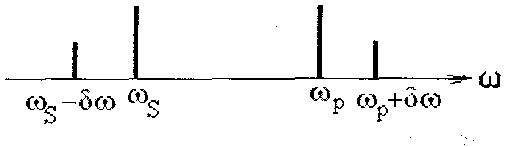
\includegraphics[width=3.43in,height=0.98in]{f137.bmp}\\
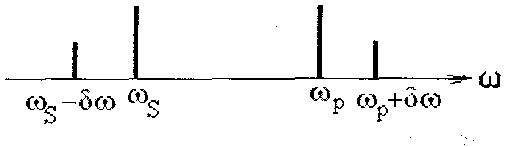
\includegraphics[width=3.43in,height=0.98in]{f137.jpg}\\
\caption{Схематическая диаграмма, демонстрирующая скачок спектра в
при усиленном ВРМБ четырехволновом смешении~\cite{1300}.}
\label{f13.7}
\end{figure}


Согласно результатам изучения лазерной интерферометрии, основанной
на ВРМБ, это частотное смещение не является преградой для
когерентного объединения пучков, усиленных в массиве параллельных
усилителей~\cite{1338}. Более того, точность совпадения оптической
длины пути в таких интерферометрах, $(\Delta l)_B$, определяется как
$(\Delta l)_B = c/(2 \pi \Delta f_B)$, и ослаблена по сравнению с
классическим интерферометрами, $(\Delta l)_c = c/(2 \pi f)$, где $f$
--- частота излучения. Для длины волны излучения $\approx1 \mu$m
$(\Delta l)_B$ и $(\Delta l)_c$ составляет $\approx3$ mm (для ВРМБ в
кварце) и $\approx0{,}1 \mu$m, соответственно.


\begin{table} [htbp]
  \centering
  \parbox{16cm}{\caption{{Использованные волоконно-оптические элементы при пассивном когерентном объединении излучения.}}
  \label{tbl_nrl_6}}
  \begin{center}
  \begin{tabular}{ | p{6cm} | p{9cm} |}
  \hline
  \hline
  Тип & Характеристики \\
  \hline
  \hline
    Многомердцевинное волокно & Высокое качество и точность составной структуры волокна \\
  \hline
    Составное зеркало &  Точность позиционирования\\
  \hline
    Фурье-линзы &  Качественное фурье-преобразование оптического сигнала \\
  \hline
  \end{tabular}
\end{center}
\end{table}


%==================================================================================

\section{Заключение}
\label{sec:anal_conclusion}

В заключении следует отметить, что за последние 2-3 года интенсивность публикаций работ по масштабированию волоконных лазеров значительно снизилась. Это может быть связано как с уже высокими достигнутыми мощностями волоконных лазеров (100 кВт от IPG), закрытостью дальнейших исследований, так и с отсутствием коммерчески доступной элементной базы для дальнейшего увеличения выходной мощности.

Что касается методов объединения излучения, то всех них можно выделить ряд общих недостатков:
\begin{itemize}
        \item реализация со стыкованными апертурами, что приводит к значительному ухудшению качества
        объединенного пучка  в дальней зоне;
        \item объединенное излучение выходит из одного волокна;
        \item взаимодействие только с ближайшими сосоедями;
        \item крайне чувствительны к невыровненности резонаторов;
        \item широкий и нестабильный выходной спектр;
        \item неопределенность в масштабируемости в плане размера (количества составляющих элементов) и мощности.
\end{itemize}

Несмотря на то, что исследования в области объединения лазерного излучения продолжаются, из проведенного анализа можно сделать некоторые выводы о желаемых идеальных характеристиках системы:
\begin{itemize}
    \item Реализация архитектуры с заполненной апертурой. Тем самым обеспечивается высокое качество обьединенного излучения в ближней и дальней зоне.
    \item Объединение излучения болжно происходить в свободном пространстве. Это возможность избавиться от фундаментальных ограничений распространения мощного лазерного излучения в кварцевой среде волокна.
    \item Узкая и стабильная ширина спектральной линии объединенного излучение. Это дает возможность распространения излучения на большие расстояния в атмосфере и подстройку длины волны.
    \item Масштабируемая пассивная техника без сложностей активной системы.
\end{itemize}

Ниже резюмируем все достоинства и недостатки проанализированных техник и методов объединения излучения волоконных лазеров.
\newpage
\begin{longtable}[c]{ | p{4cm} | p{6cm} | p{6cm} |}
  %\parbox{16cm}{\caption{Достоинства и недостатки методов объединения излучения.}
  %\label{tbl_nrl_7}}
  \hline\hline\hline
  Метод & Достоинства & Недостатки \\ \hline
   \endfirsthead   \hline
  \multicolumn{3}{|c|}{\small\slshape (продолжение)}        \\ \hline
  Метод & Достоинства & Недостатки \\ \hline
   \endhead        \hline
 \multicolumn{3}{|r|}{\small\slshape продолжение следует}  \\ \hline
    \endfoot        \hline
    \endlastfoot
  \hline\hline
    \textbf{Некогерентный: суперпозиция в дальней зоне}
    \newline\newline
    Выходы нескольких лазеров перекрываются на цели без согласования относительных фаз, длин волн или поляризации. &
    $\oplus$ Отсутствие строгих требований к длине волны, фазе или поляризации отдельных источников
    \newline$\oplus$ Возможность использования широкополосных волоконных лазеров высокой мощности
    \newline$\oplus$ Отсутствие фундаментальных пределов масштабирования размера массива
    \newline$\oplus$ Распределение интенсивности в дальней зоне не чувствительно к отказу элементов массива
    \newline$\oplus$ Продемонстрировано до 30 кВт объединенной мощности и протестировано распространение 6 кВт мощности излучения на расстояние в 1 км
    &
    $\ominus$ Ни пространственной, ни временной когерентности на выходе
    \newline$\ominus$ Требуется сложная управляемая оптика для регулировки и фокусирования излучения каждого канала
    \newline$\ominus$ В дальней зоне расхождение излучения зависит от субапертурного размера, а не объединенной апертуры
    \\
  \hline
    \textbf{Некогерентный: спектральное объединение излучения}
    \newline\newline
    Выходы массива источников, работающих с различными длинами волн, пространственно накладываются посредством фильтров или дисперсионных элементов с формированием объединенного пучка излучения.
    &
      $\oplus$ Отсутствие в методы СОИ с общим резонатором требований к длине волны, фазе или поляризации, тогда как в методах с внешним резонатором требуется только контроль за длиной волны
      \newline$\oplus$ Получение пространственно когерентного излучения, позволяющее распространяться на большие расстояния
      \newline$\oplus$ Возможен выходы с заполненной апертурой и качеством дифракционно-ограниченного излучения без <<хвотсов>> в дальней зоне
      \newline$\oplus$ Продемонстрировано до 2 кВт объединенной мощности
    &
      $\ominus$ Ухудшает спектральную чистоту отдельных лазеров
      \newline$\ominus$ В СОИ с внешним резонатором требуется точный контроль длин волн и тщательный подбор объединяющих элементов
      \newline$\ominus$ Масштабирование канала ограничивается пропускной способностью усиления активной среды
      \newline$\ominus$ Для 100 кВт иттербиевой волоконной лазерной системы требуется спектральная плотность мощности в 2 кВт/нм
      \newline$\ominus$ Обычно ограничен поглощением и искажениями на объединяющей решетке
    \\
  \hline
    \textbf{Активный когерентный}
    \newline\newline
    Включает фазовую коррекцию в реальном времени, используя оптоэлектронную обратную связь, для когерентного пространственного объединения в ближней или дальней зоне.
    &
      $\oplus$ Преимущество временно и пространственно когерентного вывода
      \newline$\oplus$  Увеличенная дистаниция распространения, интеграция с другими технологиями
      \newline$\oplus$  Продемонстрированы большие 2D массивы ($\approx$~50), теоретически масштабируем до нескольких 100 элементов
      \newline$\oplus$  Возможность регулировки выходного излучения и коррекции атмосферных искажений
      \newline$\oplus$ Продемонстрирована блокировка фазы до кВт-ых уровней мощности
    &
      $\ominus$ Требует высокой длины когерентности, узкополосных задающих источников
      \newline$\ominus$ Ограничена предельная мощность на канал
      \newline$\ominus$ Сложная электроника регулировки фазы и алгоритмы
      \newline$\ominus$ Обычно стыкованная апертура
      \newline$\ominus$ Существенная доля мощность теряется на <<хвостах>>
      \newline$\ominus$ Потребность в изоляторах высокой мощности
    \\
  \hline
    \textbf{Пассивный когерентный: интерферометрический}
    \newline\newline
    Включает размещение отдельных лазеров в интерферометре Майкельсона, обобщенного для более чем двух каналов, используя волоконные делители.
    &
      $\oplus$ Пространственно и временно когерентный вывод
      \newline$\oplus$ Не требуется сложная активная электроника регулировки фазы
      \newline$\oplus$ Цельноволоконная, устойчивая, без выравнивания система
      \newline$\oplus$ Выход с заполненной апертурой, качество дифракционно-ограниченного пучка излучения
      \newline$\oplus$ Отсутствие требований к спектральной ширине лазера
      \newline$\oplus$ Продемонстрировано эффективное объединение 4 каналов и 100 Вт объединенной мощности
    &
      $\ominus$ Выход осуществляется из одиночного волокна; масштабирование все еще ограничено фундаментальными ограничениями оптических волокон
      \newline$\ominus$ Предполагаемое недостаточное взаимодействие между несоседними элементами при древовидной архитектуре.
      \newline$\ominus$ Проблемы производства волоконных объединителей 1xN.
      \newline$\ominus$ Отсутствие четкого понимания степени и механизм самоорганизации, текущий анализ ограничен холодными резонаторами
      \newline$\ominus$ Чувствителен к отказу элементов, но сохраняет работоспособность
      \newline$\ominus$ Продемонстрировано до 8 лазеров с теоретической масштабируемостью до $\approx$~12
    \\
  \hline
    \textbf{Пассивный когерентный: пространственная фильтрация}
    \newline\newline
    Общая обратная связь осуществляется с помощью пространственной интерференционной картинки синфазных мод, отображенных на некоторой плоскости, в то время как действие несовпадающих по фазе мод в этой плоскости отфильтровывается .
    &
      $\oplus$ Пространственно и временно когерентный вывод
      \newline$\oplus$ Не требуется сложная активная электроника регулировки фазы
      \newline$\oplus$ Выходы всех лазеров интерферируют в один момент/расположение (частично справедливо для резонатора Тальба)
      \newline$\oplus$ Отсутствие требований к спектральной ширине лазеров - продемонстрировано фазирование в  большом спектральном диапазоне ($\approx$~30 нм)
      \newline$\oplus$ Работа на одной поперечной моде
      \newline$\oplus$ Совместим с многосердцевинными волокнами
      \newline$\oplus$ Продемонстрировано до 710 Вт объединенноц мощности для подхода с кольцевым резонатором
    &
      $\ominus$ \textit{Резонатор Тальбо}: Проблема дискриминации из несовпадающие по фазе мод высокого порядка для больших массивов и высоких мощностей. Архитектура стыкованной апертуры. Производственные ограничения многосердцевинных волокон. Не работает в случае одиночного отказа элемента
      \newline$\ominus$ \textit{Собственный резонатор Фурье}: Кривые профили излучения $\rightarrow$ требуются методы заполнения апертуры. Требует синфазного излучения при вводе в СФ-резонатор для качественного преобразования. Масштабируемость массива требует более низких коэффициентов заполнения. Возможно, не работает в случае одиночного отказа элемента
      \newline$\ominus$ \textit{Кольцевой резонатор}: плохое качество излучения в дальней зоне, связанное с архитектурой стыкованной апертуры. Не понятная степень масштабируемости массива.
    \\
  \hline
\end{longtable}

Что касается использованных волоконно-оптических компонентов, то, исходя из общих технических требований к качеству и стабильности излучения лазерных комплексов, в целом они должны обеспечивать:
\begin{itemize}
    \item Высокую энергетическую эффективность преобразования лазерного пучка, высокое оптическое качество пучка.
    \item Высокую временную стабильность мощности выводимого лазерного излучения и пространственно-временную стабильность осевого положения пучка, а также его модового состава.
    \item Пространственно-временную форму распределения интенсивности излучения на цели, необходимую для выполнения задач лазерного технологического процесса.
    \item В отдельных случая ВОЭ должны обеспечивать спектральную селективность или необходимые поляризационные характеристики лазерного излучения.
    \item Конструкции ВОЭ должны обеспечивать высокий эксплуатационный ресурс как самих элементов, так и других составных частей лазеров, а также удобство и функциональность при обслуживании и юстировке.
\end{itemize}
В отчете также приведены общие и специфические для каждого метода объединения требования к ВОЭ в лазерных системах высокой мощности.

В применение к задачам, решаемым в РФЯЦ-ВНИИТФ, для увеличения мощности имеющихся волоконных лазеров стоит предложить следующее:
\begin{enumerate}
\item Продолжать работы по \textit{увеличению мощности модулей накачки высокой яркости}. Стоит ожидать получения модулей с выходной мощность 100 Вт из волокна 105/125 мкм (NA=0,15). Однако, при сохранении существующих габаритных размеров подобный рост не представляется возможным без освоения монтажа распределенных линеек лазерных диодов и их последующего облинзовывания, а также свободного доступа к качественным просветленным микролинзам. Наряду с этим на данный момент видится предпочтительным остановится на модулях средней мощности (до 50 Вт) и сконцентрироваться на повышении их надежности и качества выходного излучения, а также оптимизации массогабаритов и системы теплоотвода.
\item  \textit{Когерентное сложение} все еще остается действенным и реализуемым методом получения мультикиловаттных волоконных лазеров. В первую очередь следует обратить внимание на методы оценки качества полученной интерференционной картины – получение количественной оценки ее контрастности. Применяемая на данный момент визуальная оценка не корректна. Кроме того, для качественного когерентного сложения необходима количественная оценка фазового шума. Из анализа литературы видно, что подобная задача хоть и достаточно проработана, но тем не менее крайне сложна как в теоретическом, так и экспериментальном плане. Однако без ее решения остается не понятным на сколько в фазовом модуляторе необходимо скорректировать фазу без оценки ее ошибки. Без оценок фазового шума и контрастности движение вперед в данном вопросе будет неконструктивным.
\item  \textit{Спектральное объединение излучения} также достаточно перспективно. Основной сложностью в применении данной методики является отсутствие объемных брэгговских решеток хорошего качества от отечественных производителей (ИТМО и ГОИ), а применение зарубежных (OptiGrate, США) может быть дорогим и затруднительным в ряде решаемых задач. Кроме того, спектральное сложение требует большого экспериментального мастерства и опыта в работе с объемной оптикой и дифракционными элементами. Также известно, что в коммерческом доступе существуют только решетки для невысоких мощностей (десятки ватт), далее необходимо применять системы охлаждения, которая у производителя есть, но она коммерчески не доступна. Иными словами, для мультикиловаттных волоконных лазерных систем необходима разрабатывать систему охлаждения объемной оптики. Несмотря на все вышесказанное работу в данном направлении нужно начинать скорейшим образом.
\item  Основным реальным способом масштабирования волоконных лазеров РФЯЦ-ВНИИТФ видится в \textit{некогерентном объединении излучения} с помощью сплавленных волоконных объединителей. Интенсивность работ по их созданию необходимо значительно усилить, так как спектр коммерчески доступных волоконных объединителей накачки и сигнала с ростом мощности лазеров сильно уменьшается, а стоимость их крайне высока.
\end{enumerate}

В конце хотелось бы обратить внимание на важность в ходе  выполнения НИР и ОКР по лазерным системам различного применения учитывать требования экономики изготовления как самих лазеров, так и составляющих ВОЭ. Эти требования включают:
\begin{itemize}
    \item Модульность конструкции.
    \item Максимальное использование готовых промышленных выпускаемых комплектующих и узлов и изделий.
    \item Унификацию и стандартизацию лазера и его комплектующих.
    \item Использование недорогих и недефицитных материалов в конструкции.
    \item Высокий уровень конструкторской проработки, заключающийся
    \begin{itemize}
    \item в минимальном числе отдельных блоков;
    \item в максимальном обеспечении необходимыми в эксплуатации механическими, оптическими и электронными аксессуарами;
    \item в оптимальном сопряжении лазера с остальными частями лазерного (технологического) комплекса;
    \item в разумном соотношении универсализации и специализации.
    \end{itemize}
\end{itemize}


\clearpage
